% Options for packages loaded elsewhere
\PassOptionsToPackage{unicode}{hyperref}
\PassOptionsToPackage{hyphens}{url}
%
\documentclass[
]{article}
\usepackage{amsmath,amssymb}
\usepackage{iftex}
\ifPDFTeX
  \usepackage[T1]{fontenc}
  \usepackage[utf8]{inputenc}
  \usepackage{textcomp} % provide euro and other symbols
\else % if luatex or xetex
  \usepackage{unicode-math} % this also loads fontspec
  \defaultfontfeatures{Scale=MatchLowercase}
  \defaultfontfeatures[\rmfamily]{Ligatures=TeX,Scale=1}
\fi
\usepackage{lmodern}
\ifPDFTeX\else
  % xetex/luatex font selection
\fi
% Use upquote if available, for straight quotes in verbatim environments
\IfFileExists{upquote.sty}{\usepackage{upquote}}{}
\IfFileExists{microtype.sty}{% use microtype if available
  \usepackage[]{microtype}
  \UseMicrotypeSet[protrusion]{basicmath} % disable protrusion for tt fonts
}{}
\makeatletter
\@ifundefined{KOMAClassName}{% if non-KOMA class
  \IfFileExists{parskip.sty}{%
    \usepackage{parskip}
  }{% else
    \setlength{\parindent}{0pt}
    \setlength{\parskip}{6pt plus 2pt minus 1pt}}
}{% if KOMA class
  \KOMAoptions{parskip=half}}
\makeatother
\usepackage{xcolor}
\usepackage[margin=1in]{geometry}
\usepackage{color}
\usepackage{fancyvrb}
\newcommand{\VerbBar}{|}
\newcommand{\VERB}{\Verb[commandchars=\\\{\}]}
\DefineVerbatimEnvironment{Highlighting}{Verbatim}{commandchars=\\\{\}}
% Add ',fontsize=\small' for more characters per line
\usepackage{framed}
\definecolor{shadecolor}{RGB}{248,248,248}
\newenvironment{Shaded}{\begin{snugshade}}{\end{snugshade}}
\newcommand{\AlertTok}[1]{\textcolor[rgb]{0.94,0.16,0.16}{#1}}
\newcommand{\AnnotationTok}[1]{\textcolor[rgb]{0.56,0.35,0.01}{\textbf{\textit{#1}}}}
\newcommand{\AttributeTok}[1]{\textcolor[rgb]{0.13,0.29,0.53}{#1}}
\newcommand{\BaseNTok}[1]{\textcolor[rgb]{0.00,0.00,0.81}{#1}}
\newcommand{\BuiltInTok}[1]{#1}
\newcommand{\CharTok}[1]{\textcolor[rgb]{0.31,0.60,0.02}{#1}}
\newcommand{\CommentTok}[1]{\textcolor[rgb]{0.56,0.35,0.01}{\textit{#1}}}
\newcommand{\CommentVarTok}[1]{\textcolor[rgb]{0.56,0.35,0.01}{\textbf{\textit{#1}}}}
\newcommand{\ConstantTok}[1]{\textcolor[rgb]{0.56,0.35,0.01}{#1}}
\newcommand{\ControlFlowTok}[1]{\textcolor[rgb]{0.13,0.29,0.53}{\textbf{#1}}}
\newcommand{\DataTypeTok}[1]{\textcolor[rgb]{0.13,0.29,0.53}{#1}}
\newcommand{\DecValTok}[1]{\textcolor[rgb]{0.00,0.00,0.81}{#1}}
\newcommand{\DocumentationTok}[1]{\textcolor[rgb]{0.56,0.35,0.01}{\textbf{\textit{#1}}}}
\newcommand{\ErrorTok}[1]{\textcolor[rgb]{0.64,0.00,0.00}{\textbf{#1}}}
\newcommand{\ExtensionTok}[1]{#1}
\newcommand{\FloatTok}[1]{\textcolor[rgb]{0.00,0.00,0.81}{#1}}
\newcommand{\FunctionTok}[1]{\textcolor[rgb]{0.13,0.29,0.53}{\textbf{#1}}}
\newcommand{\ImportTok}[1]{#1}
\newcommand{\InformationTok}[1]{\textcolor[rgb]{0.56,0.35,0.01}{\textbf{\textit{#1}}}}
\newcommand{\KeywordTok}[1]{\textcolor[rgb]{0.13,0.29,0.53}{\textbf{#1}}}
\newcommand{\NormalTok}[1]{#1}
\newcommand{\OperatorTok}[1]{\textcolor[rgb]{0.81,0.36,0.00}{\textbf{#1}}}
\newcommand{\OtherTok}[1]{\textcolor[rgb]{0.56,0.35,0.01}{#1}}
\newcommand{\PreprocessorTok}[1]{\textcolor[rgb]{0.56,0.35,0.01}{\textit{#1}}}
\newcommand{\RegionMarkerTok}[1]{#1}
\newcommand{\SpecialCharTok}[1]{\textcolor[rgb]{0.81,0.36,0.00}{\textbf{#1}}}
\newcommand{\SpecialStringTok}[1]{\textcolor[rgb]{0.31,0.60,0.02}{#1}}
\newcommand{\StringTok}[1]{\textcolor[rgb]{0.31,0.60,0.02}{#1}}
\newcommand{\VariableTok}[1]{\textcolor[rgb]{0.00,0.00,0.00}{#1}}
\newcommand{\VerbatimStringTok}[1]{\textcolor[rgb]{0.31,0.60,0.02}{#1}}
\newcommand{\WarningTok}[1]{\textcolor[rgb]{0.56,0.35,0.01}{\textbf{\textit{#1}}}}
\usepackage{longtable,booktabs,array}
\usepackage{calc} % for calculating minipage widths
% Correct order of tables after \paragraph or \subparagraph
\usepackage{etoolbox}
\makeatletter
\patchcmd\longtable{\par}{\if@noskipsec\mbox{}\fi\par}{}{}
\makeatother
% Allow footnotes in longtable head/foot
\IfFileExists{footnotehyper.sty}{\usepackage{footnotehyper}}{\usepackage{footnote}}
\makesavenoteenv{longtable}
\usepackage{graphicx}
\makeatletter
\def\maxwidth{\ifdim\Gin@nat@width>\linewidth\linewidth\else\Gin@nat@width\fi}
\def\maxheight{\ifdim\Gin@nat@height>\textheight\textheight\else\Gin@nat@height\fi}
\makeatother
% Scale images if necessary, so that they will not overflow the page
% margins by default, and it is still possible to overwrite the defaults
% using explicit options in \includegraphics[width, height, ...]{}
\setkeys{Gin}{width=\maxwidth,height=\maxheight,keepaspectratio}
% Set default figure placement to htbp
\makeatletter
\def\fps@figure{htbp}
\makeatother
\setlength{\emergencystretch}{3em} % prevent overfull lines
\providecommand{\tightlist}{%
  \setlength{\itemsep}{0pt}\setlength{\parskip}{0pt}}
\setcounter{secnumdepth}{5}
\usepackage{pdfpages}
\usepackage{fontspec}
\setmainfont{Times New Roman}
\ifLuaTeX
  \usepackage{selnolig}  % disable illegal ligatures
\fi
\usepackage{bookmark}
\IfFileExists{xurl.sty}{\usepackage{xurl}}{} % add URL line breaks if available
\urlstyle{same}
\hypersetup{
  hidelinks,
  pdfcreator={LaTeX via pandoc}}

\author{}
\date{\vspace{-2.5em}}

\begin{document}


\includepdf[pages=1]{bia.pdf}
\pagenumbering{gobble}

\newpage
\thispagestyle{empty}

\begin{center}
    \LARGE \textbf{LỜI CAM ĐOAN}
\end{center}
\vspace{1.5em}

Chúng tôi, \textbf{Bùi Minh Huy}, \textbf{Trần Lê Vân}, \textbf{Nguyễn
Thị Thanh Tâm} xin cam đoan rằng:

Tất cả thông tin và phân tích trình bày trong báo cáo này được thực hiện
một cách chính xác và trung thực. Mọi dữ liệu, nhận định hoặc ý kiến
được trích dẫn từ các nguồn khác đều đã được nêu rõ nguồn gốc và trích
dẫn đúng quy định. Chúng tôi cam đoan rằng không có bất kỳ hành vi sao
chép hoặc sử dụng thông tin không hợp pháp nào từ các nguồn khác. Bài
báo cáo này là kết quả của công trình nghiên cứu độc lập của chúng tôi
và chưa từng được công bố tại bất kỳ nơi nào khác. Chúng tôi cam đoan đã
tuân thủ nghiêm ngặt các quy tắc và quy định của môn học, bao gồm việc
tham khảo và áp dụng các công cụ nghiên cứu một cách hợp lệ. Nếu phát
hiện có bất kỳ sự gian lận nào, chúng tôi xin hoàn toàn chịu trách nhiệm
về nội dung bài báo cáo của mình. Chúng tôi hy vọng rằng bài báo cáo này
sẽ cung cấp những thông tin hữu ích cho các nhà nghiên cứu, doanh
nghiệp, góp phần vào việc hiểu rõ hơn về mạng xã hội ngày nay.

\vspace{3em}

\begin{flushright}
\begin{minipage}{0.5\textwidth}
\raggedleft
TP.\ Hồ Chí Minh, ngày 28 tháng 3 năm 2025

\vspace{1em}

\centering
\textbf{\LARGE Sinh viên}
\end{minipage}
\end{flushright}

\newpage
\thispagestyle{empty}
\tableofcontents
\newpage
\pagenumbering{arabic}
\setcounter{page}{1}

\section{Abstract}\label{abstract}

\section{Introduction}\label{introduction}

Trong thời đại của điện toán di động và thiết bị thông minh, việc theo
dõi và nhận dạng hoạt động con người (Human Activity Recognition - HAR)
đã trở thành một lĩnh vực nghiên cứu đóng vai trò quan trọng trong nhiều
ngành như trí tuệ nhân tạo, khoa học dữ liệu, y học và công nghệ cảm
biến. HAR đóng vai trò cốt lõi trong các ứng dụng như giám sát sức khỏe,
phát hiện té ngã, điều khiển nhà thông minh. Ngày nay, nhu cầu càng ngày
gia tăng về các thiết bị công nghệ có thể hiểu hành vi con người dẫn đến
việc phát triển các mô hình HAR là chính xác, hiệu quả và có khả năng
triển khai thực tế là vô cùng cần thết.

Một trong những yếu tố chính thúc đẩy sự phát triển của HẢ là sự phổ
biến của các thiết bị di động thông minh và đồng hồ thông minh, vốn đợc
trang bị sẵn các cảm biến quán tính bao gồm gia tốc kế (accelerometer)
và con quay hồi chuyển (gyroscope). Những cảm biến này cho phép thu thập
dữ liệu về chuyển động của người sử dụng với độ chính xác cao, chi phí
thấp và tính khả dụng cao trong đời sống hàng ngày. Nhờ vậy, hệ thống
HAR có thể được lắp đặt mà không cần sử dụng các thiết bị đắt tiền hoặc
lắp đặt phức tạp.

Bên cạnh tiềm năng ứng dụng rộng rãi, việc xây dựng các mô hình HAR vẫn
có nhiều khó khăn thách thức như dữ liệu cảm biến thường có số chiều
lớn, có nhiều dữ liệu nhiễu và có tính biến động cao do phụ thuộc vào
thói quen và hình thể của mỗi người. Bên cạnh đó, một số hoạt động có
thể có mẫu tín hiệu tương tự nhau khiến cho các bài toán phân loại trở
nên khó khăn hơn. Vì vậy, cần có một quy trình xử lý dữ liệu bài bản bao
gồm các bước tiền xử lý dữ liệu, giảm chiều dữ liệu và huấn luyện mô
hình học máy để có thể đặt được hiệu quả cao trong việc nhận dạng hoạt
động con người.

Trong nghiên cứu này, chúng em đã tiến hành khai thác bộ dữ liệu
``\textbf{Human Activity Recognition with Smartphones}'' do UCI Machine
Learning Repository cung cấp, một bộ dữ liệu được sử dụng rộng raix
trong cộng đồng nghiên cứu HAR. Chúng em đề xuất một quy trình học máy
toàn diện bao gồm phân tích đặc trưng, giảm chiều dữ liệu bằng UMAP,
PCA, TSNE và huấn luyện bằng các mô hình học máy như Random Forest,
Decision Tree, Logistic Regression, Support Vectot Machine (SVM) để phân
loại các hoạt động với mục tiêu là nâng cao độ chính xác và hiệu quả của
mô hình. Những kết quả này sẽ cung cấp cái nhìn thực nghiệm rõ ràng cho
các nhà nghiên cứu, đồng thời làm nền móng cho việc triển khai các hệ
thống nhận dạng hoạt động trong thế giới thực.

\section{Dataset and Preprocessing (Dữ liệu và tiền xử
lý)}\label{dataset-and-preprocessing-dux1eef-liux1ec7u-vuxe0-tiux1ec1n-xux1eed-luxfd}

Bộ dữ liệu \textbf{Human Activity Recognition with Smartphones} được thu
thập từ 30 người tham gia (gọi là \emph{subjects}) (15 nam và 15 nữ, độ
tuổi từ 19 đến 48) thực hiện sáu hoạt động thường ngày như Đi bộ
(Walking), đi lên cầu thang (Walking Upstairs), đi xuống cầu thang
(WalkingDownstairs), ngồi (Sitting),đứng (Standing),nằm (Laying). Dữ
liệu được ghi lại bằng một điện thoại thông minh (Samsung Galaxy S II)
đeo ở thắt lưng của người dùng. Các cảm biến gồm \textbf{accelerometer}
và \textbf{gyroscope} được sử dụng để ghi lại chuyển động theo 3 trục X,
Y, Z với tần suất 50Hz.

Mỗi chuỗi tín hiệu được chia thành các \textbf{cửa sổ trượt} có độ dài
2.56 giây, tương ứng với 128 lần đo. Từ mỗi cửa sổ, các đặc trưng
(features) đã được trích xuất từ \textbf{miền thời gian} và \textbf{miền
tần số} để tạo ra một tập hợp dữ liệu có cấu trúc sẵn sàng cho mô hình
học máy.

Các nhóm tín hiệu chính bao gồm:

\begin{itemize}
\tightlist
\item
  \texttt{tBodyAcc-XYZ}: Gia tốc cơ thể theo 3 trục trong miền thời
  gian\\
\item
  \texttt{tGravityAcc-XYZ}: Gia tốc do trọng lực\\
\item
  \texttt{tBodyGyro-XYZ}: Tốc độ quay từ con quay hồi chuyển\\
\item
  \texttt{tBodyAccJerk-XYZ}, \texttt{tBodyGyroJerk-XYZ}: Jerk - đo sự
  thay đổi đột ngột của chuyển động\\
\item
  \texttt{Mag}: Độ lớn vector gia tốc, được tính bằng chuẩn Euclidean:\\
  \[
  \text{Mag} = \sqrt{X^2 + Y^2 + Z^2}
  \]
\item
  \texttt{fBodyAcc-XYZ}, \texttt{fBodyGyro-XYZ}: Biến miền tần số được
  tạo từ FFT
\end{itemize}

Từ các tín hiệu trên, một loạt đặc trưng thống kê được tính toán như:

\begin{itemize}
\item
  \texttt{mean()}, \texttt{std()}, \texttt{mad()}, \texttt{max()},
  \texttt{min()}
\item
  \texttt{sma()}: Signal Magnitude Area
\item
  \texttt{energy()}: Tổng bình phương chia số phần tử
\item
  \texttt{entropy()}, \texttt{iqr()}, \texttt{arCoeff()},
  \texttt{correlation()}
\item
  \texttt{meanFreq()}, \texttt{skewness()}, \texttt{kurtosis()},
  \texttt{bandsEnergy()}, \texttt{angle()}

  Toàn bộ bộ dữ liệu được chia thành hai phần: Tập huấn luyện
  (train.csv): bao gồm 7352 mẫu. Tập kiểm tra (test.csv): bao gồm 2947
  mẫu. Mỗi mẫu tương ứng với một cửa sổ thời gian 2.56 giây, được biểu
  diễn bằng \textbf{561 đặc trưng đầu vào (features)}, 1mỗi mẫu còn bao
  gồm một mã định danh người thực hiện (subject) và một nhãn hoạt động
  (Activity), ác nhãn này được mã hóa từ 1 đến 6 tương ứng với:
\end{itemize}

\begin{longtable}[]{@{}ll@{}}
\toprule\noalign{}
Giá trị nhãn & Hoạt động \\
\midrule\noalign{}
\endhead
\bottomrule\noalign{}
\endlastfoot
1 & WALKING \\
2 & WALKING\_UPSTAIRS \\
3 & WALKING\_DOWNSTAIRS \\
4 & SITTING \\
5 & STANDING \\
6 & LAYING \\
\end{longtable}

\begin{Shaded}
\begin{Highlighting}[]
\CommentTok{\# install.packages("showtext")}
\CommentTok{\# install.packages("ggplot2")}
\end{Highlighting}
\end{Shaded}

\begin{Shaded}
\begin{Highlighting}[]
\CommentTok{\# train \textless{}{-}read.csv(\textquotesingle{}/Users/huy/Documents/doanthaytung/archive/train.csv\textquotesingle{})}
\CommentTok{\# train \textless{}{-}read.csv("D:/BT/clonegit/doanthaytung/archive/train.csv")}
\NormalTok{train }\OtherTok{\textless{}{-}} \FunctionTok{read.csv}\NormalTok{(}\StringTok{\textquotesingle{}archive/train.csv\textquotesingle{}}\NormalTok{)}
\CommentTok{\# head(train)}
\FunctionTok{dim}\NormalTok{(train)}
\end{Highlighting}
\end{Shaded}

\begin{verbatim}
## [1] 7352  563
\end{verbatim}

\begin{Shaded}
\begin{Highlighting}[]
\CommentTok{\# test \textless{}{-}read.csv(\textquotesingle{}/Users/huy/Documents/doanthaytung/archive/test.csv\textquotesingle{})}
\CommentTok{\# test \textless{}{-}read.csv("D:/BT/clonegit/doanthaytung/archive/test.csv")}
\NormalTok{test }\OtherTok{\textless{}{-}} \FunctionTok{read.csv}\NormalTok{(}\StringTok{"archive/test.csv"}\NormalTok{)}
\CommentTok{\# head(test)}
\FunctionTok{dim}\NormalTok{(test)}
\end{Highlighting}
\end{Shaded}

\begin{verbatim}
## [1] 2947  563
\end{verbatim}

xem các các type có trong data

\begin{Shaded}
\begin{Highlighting}[]
\FunctionTok{table}\NormalTok{(}\FunctionTok{sapply}\NormalTok{(train, class))}
\end{Highlighting}
\end{Shaded}

\begin{verbatim}
## 
## character   integer   numeric 
##         1         1       561
\end{verbatim}

in ra cột có dạng charactor

\begin{Shaded}
\begin{Highlighting}[]
\FunctionTok{names}\NormalTok{(train)[}\FunctionTok{sapply}\NormalTok{(train, class) }\SpecialCharTok{==} \StringTok{"character"}\NormalTok{]}
\end{Highlighting}
\end{Shaded}

\begin{verbatim}
## [1] "Activity"
\end{verbatim}

\begin{Shaded}
\begin{Highlighting}[]
\FunctionTok{unique}\NormalTok{(train}\SpecialCharTok{$}\NormalTok{Activity)}
\end{Highlighting}
\end{Shaded}

\begin{verbatim}
## [1] "STANDING"           "SITTING"            "LAYING"            
## [4] "WALKING"            "WALKING_DOWNSTAIRS" "WALKING_UPSTAIRS"
\end{verbatim}

chuyển thành factor

\begin{Shaded}
\begin{Highlighting}[]
\NormalTok{train}\SpecialCharTok{$}\NormalTok{Activity }\OtherTok{\textless{}{-}} \FunctionTok{as.factor}\NormalTok{(train}\SpecialCharTok{$}\NormalTok{Activity)}
\NormalTok{test}\SpecialCharTok{$}\NormalTok{Activity }\OtherTok{\textless{}{-}} \FunctionTok{as.factor}\NormalTok{(test}\SpecialCharTok{$}\NormalTok{Activity)}
\end{Highlighting}
\end{Shaded}

\begin{Shaded}
\begin{Highlighting}[]
\FunctionTok{cat}\NormalTok{(}\StringTok{"Giá trị thiếu ở tập train:"}\NormalTok{, }\FunctionTok{sum}\NormalTok{(}\FunctionTok{is.na}\NormalTok{(train)), }\StringTok{"}\SpecialCharTok{\textbackslash{}n}\StringTok{"}\NormalTok{)}
\end{Highlighting}
\end{Shaded}

\begin{verbatim}
## Giá trị thiếu ở tập train: 0
\end{verbatim}

\begin{Shaded}
\begin{Highlighting}[]
\FunctionTok{cat}\NormalTok{(}\StringTok{"Giá trị thiếu ở tập test:"}\NormalTok{, }\FunctionTok{sum}\NormalTok{(}\FunctionTok{is.na}\NormalTok{(test)), }\StringTok{"}\SpecialCharTok{\textbackslash{}n}\StringTok{"}\NormalTok{)}
\end{Highlighting}
\end{Shaded}

\begin{verbatim}
## Giá trị thiếu ở tập test: 0
\end{verbatim}

\begin{Shaded}
\begin{Highlighting}[]
\FunctionTok{cat}\NormalTok{(}\StringTok{"Số dòng bị trùng lặp trong tập train:"}\NormalTok{, }\FunctionTok{sum}\NormalTok{(}\FunctionTok{duplicated}\NormalTok{(train)), }\StringTok{"}\SpecialCharTok{\textbackslash{}n}\StringTok{"}\NormalTok{)}
\end{Highlighting}
\end{Shaded}

\begin{verbatim}
## Số dòng bị trùng lặp trong tập train: 0
\end{verbatim}

\begin{Shaded}
\begin{Highlighting}[]
\FunctionTok{cat}\NormalTok{(}\StringTok{"Số dòng bị trùng lặp trong tập test :"}\NormalTok{, }\FunctionTok{sum}\NormalTok{(}\FunctionTok{duplicated}\NormalTok{(test)), }\StringTok{"}\SpecialCharTok{\textbackslash{}n}\StringTok{"}\NormalTok{)}
\end{Highlighting}
\end{Shaded}

\begin{verbatim}
## Số dòng bị trùng lặp trong tập test : 0
\end{verbatim}

\begin{Shaded}
\begin{Highlighting}[]
\FunctionTok{library}\NormalTok{(ggplot2)}
\FunctionTok{library}\NormalTok{(showtext)}
\end{Highlighting}
\end{Shaded}

\begin{verbatim}
## Loading required package: sysfonts
\end{verbatim}

\begin{verbatim}
## Loading required package: showtextdb
\end{verbatim}

\begin{Shaded}
\begin{Highlighting}[]
\FunctionTok{showtext\_auto}\NormalTok{()}

\FunctionTok{ggplot}\NormalTok{(train, }\FunctionTok{aes}\NormalTok{(}\AttributeTok{x =} \FunctionTok{factor}\NormalTok{(subject), }\AttributeTok{fill =}\NormalTok{ Activity)) }\SpecialCharTok{+}
  \FunctionTok{geom\_bar}\NormalTok{(}\AttributeTok{position =} \StringTok{"dodge"}\NormalTok{, }\AttributeTok{width =} \FloatTok{0.7}\NormalTok{) }\SpecialCharTok{+}
  \FunctionTok{scale\_fill\_brewer}\NormalTok{(}\AttributeTok{palette =} \StringTok{"Set2"}\NormalTok{) }\SpecialCharTok{+} 
  \FunctionTok{labs}\NormalTok{(}
    \AttributeTok{title =} \StringTok{"Số lượng mẫu dữ liệu theo người dùng và hoạt động"}\NormalTok{,}
    \AttributeTok{x =} \StringTok{"Người dùng (Subject)"}\NormalTok{,}
    \AttributeTok{y =} \StringTok{"Số lượng mẫu"}\NormalTok{,}
    \AttributeTok{fill =} \StringTok{"Hoạt động"}
\NormalTok{  ) }\SpecialCharTok{+}
  \FunctionTok{theme\_minimal}\NormalTok{(}\AttributeTok{base\_size =} \DecValTok{16}\NormalTok{) }\SpecialCharTok{+}
  \FunctionTok{theme}\NormalTok{(}
    \AttributeTok{plot.title =} \FunctionTok{element\_text}\NormalTok{(}\AttributeTok{hjust =} \FloatTok{0.5}\NormalTok{, }\AttributeTok{face =} \StringTok{"bold"}\NormalTok{, }\AttributeTok{size =} \DecValTok{20}\NormalTok{),}
    \AttributeTok{axis.text.x =} \FunctionTok{element\_text}\NormalTok{(}\AttributeTok{angle =} \DecValTok{45}\NormalTok{, }\AttributeTok{hjust =} \DecValTok{1}\NormalTok{),}
    \AttributeTok{legend.position =} \StringTok{"right"}
\NormalTok{  )}
\end{Highlighting}
\end{Shaded}

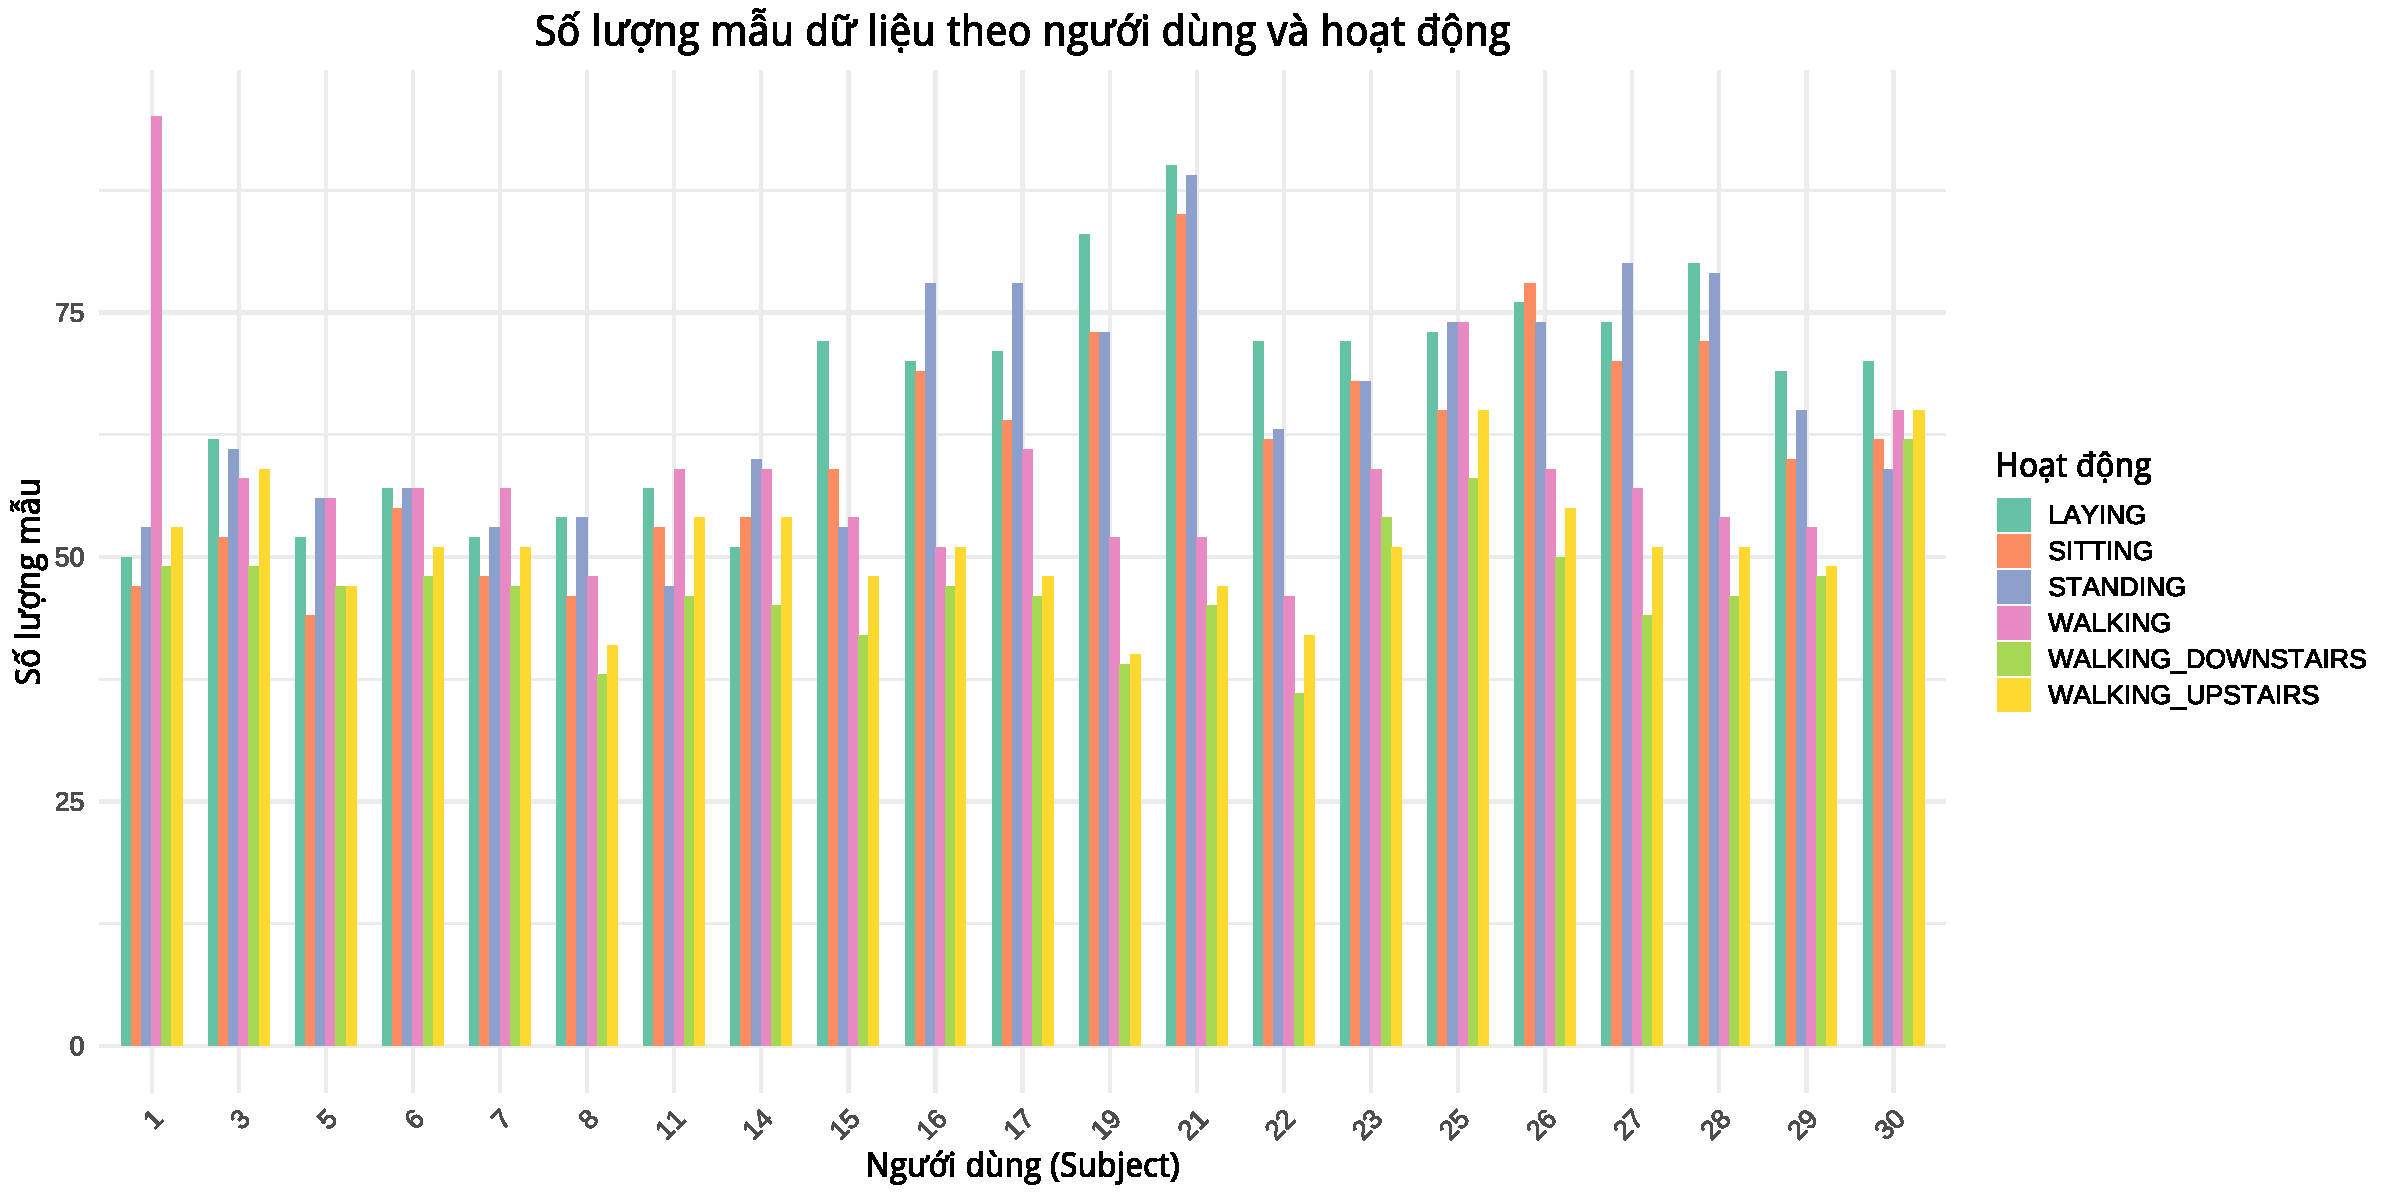
\includegraphics{report_files/figure-latex/unnamed-chunk-10-1.pdf}

\begin{Shaded}
\begin{Highlighting}[]
\FunctionTok{library}\NormalTok{(ggplot2)}

\FunctionTok{ggplot}\NormalTok{(train, }\FunctionTok{aes}\NormalTok{(}\AttributeTok{x =}\NormalTok{ Activity, }\AttributeTok{fill =}\NormalTok{ Activity)) }\SpecialCharTok{+}
  \FunctionTok{geom\_bar}\NormalTok{() }\SpecialCharTok{+}
  \FunctionTok{labs}\NormalTok{(}
    \AttributeTok{title =} \StringTok{"Số lượng mẫu theo từng hoạt động"}\NormalTok{,}
    \AttributeTok{x =} \StringTok{"Hoạt động"}\NormalTok{,}
    \AttributeTok{y =} \StringTok{"Số lượng mẫu"}
\NormalTok{  ) }\SpecialCharTok{+}
  \FunctionTok{theme\_minimal}\NormalTok{(}\AttributeTok{base\_size =} \DecValTok{15}\NormalTok{) }\SpecialCharTok{+}
  \FunctionTok{theme}\NormalTok{(}
    \AttributeTok{axis.text.x =} \FunctionTok{element\_text}\NormalTok{(}\AttributeTok{angle =} \DecValTok{45}\NormalTok{, }\AttributeTok{vjust =} \DecValTok{1}\NormalTok{, }\AttributeTok{hjust=}\DecValTok{1}\NormalTok{),}
    \AttributeTok{plot.title =} \FunctionTok{element\_text}\NormalTok{(}\AttributeTok{hjust =} \FloatTok{0.5}\NormalTok{, }\AttributeTok{face =} \StringTok{"bold"}\NormalTok{)}
\NormalTok{  ) }\SpecialCharTok{+}
  \FunctionTok{guides}\NormalTok{(}\AttributeTok{fill =} \StringTok{"none"}\NormalTok{)}
\end{Highlighting}
\end{Shaded}

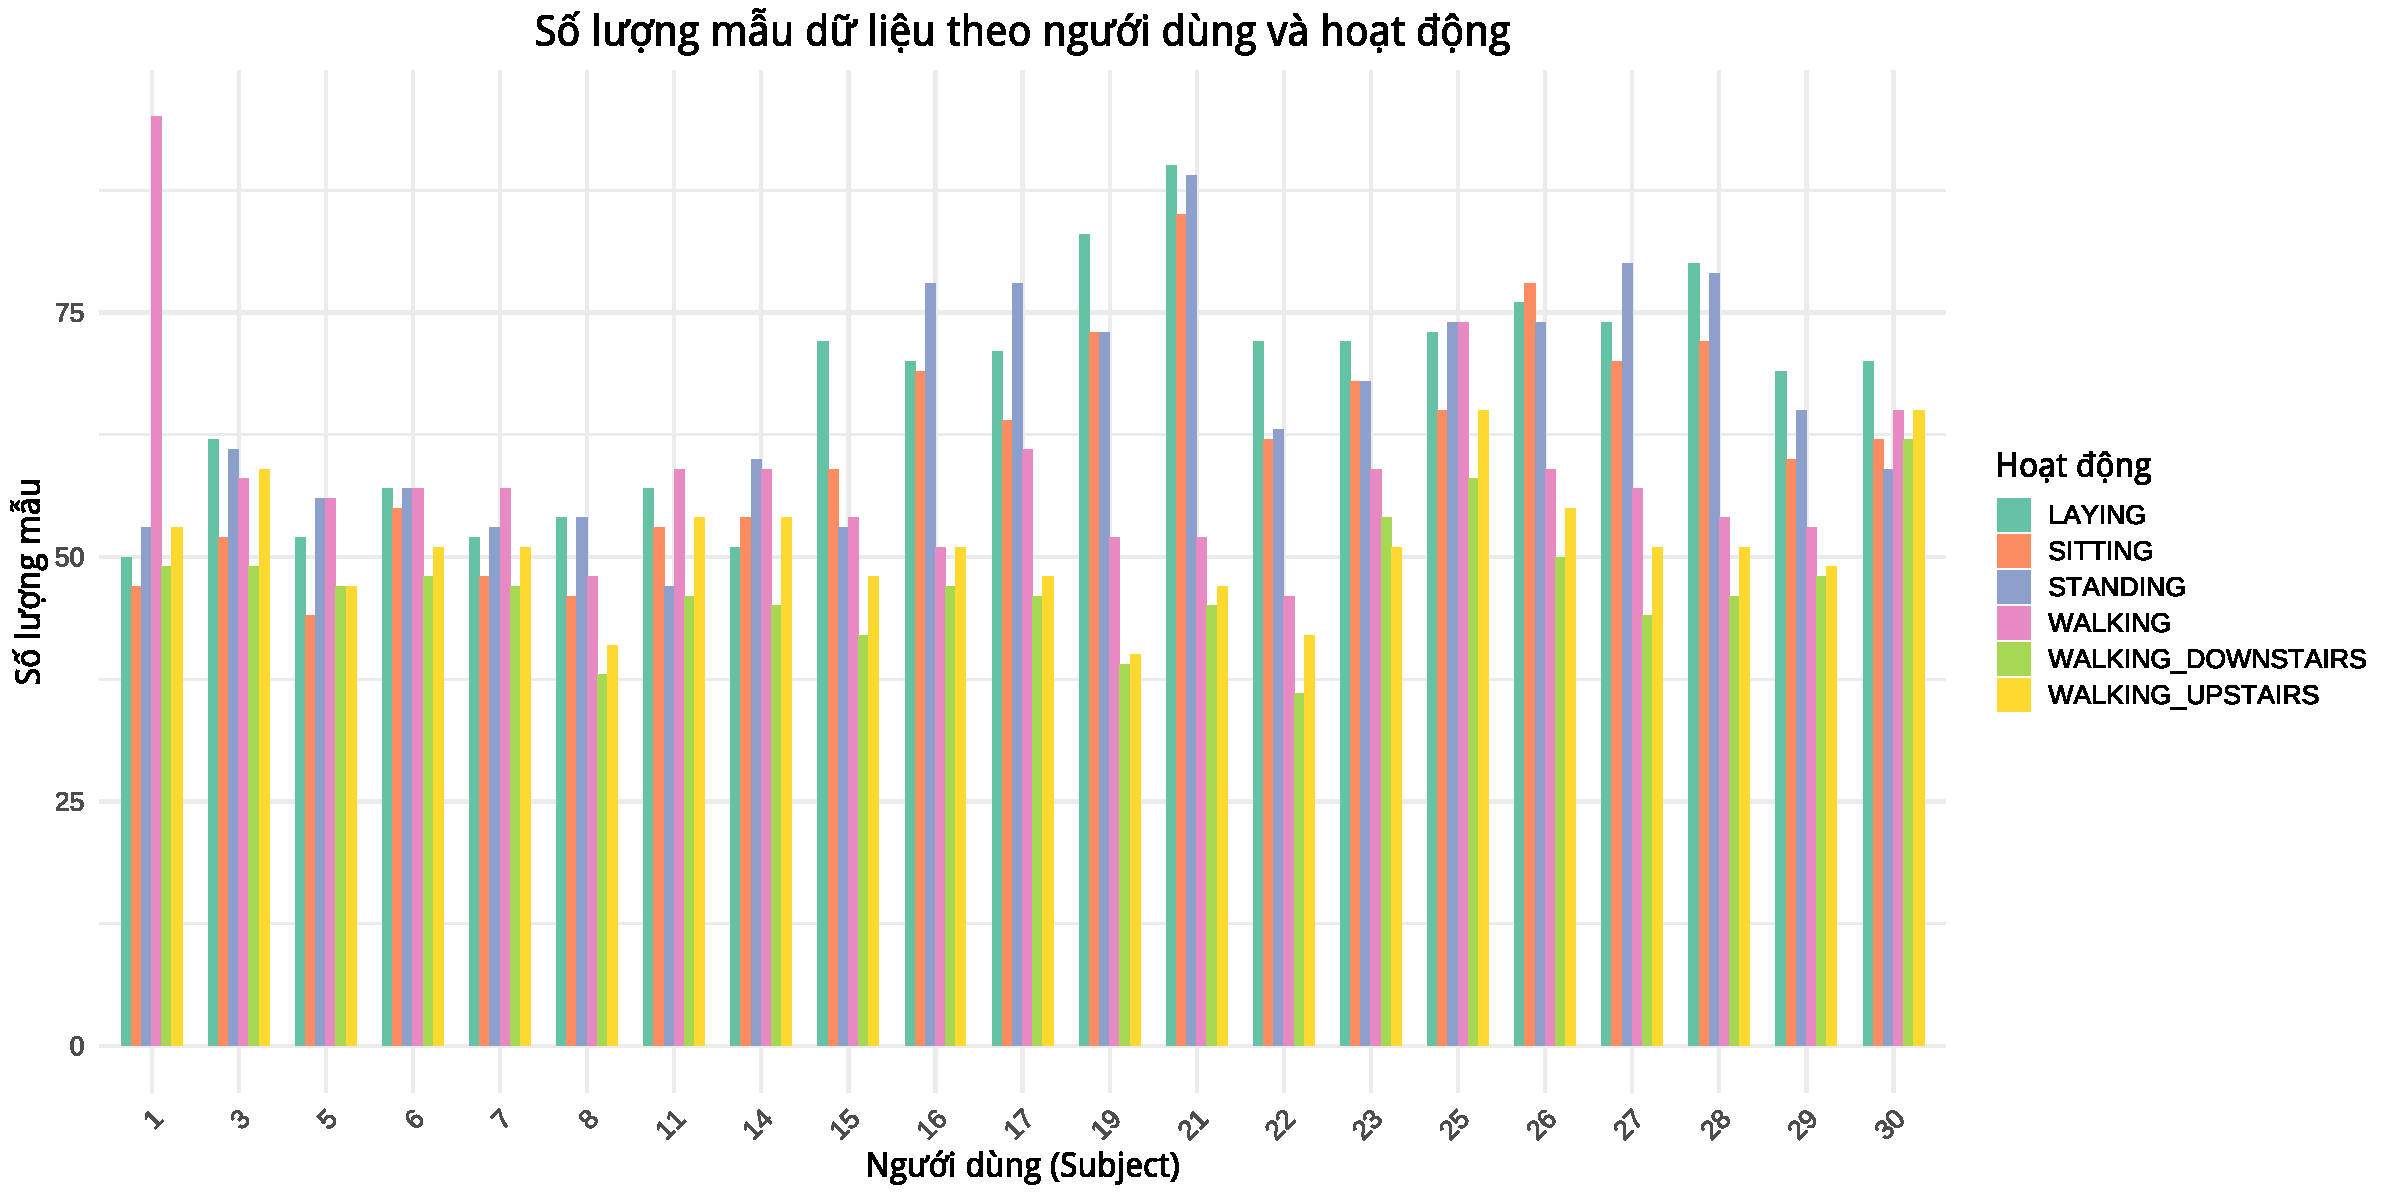
\includegraphics{report_files/figure-latex/unnamed-chunk-11-1.pdf} Số
lượng mẫu cho mỗi hoạt động dao động trong khoảng 1000 mẫu đến 1200 mẫu.
Các hoạt động tĩnh như laying, sitting, standing có xu hướng chiếm tỷ lệ
cao hơn một chút so với các hoạt động di chuyển như walking,
walking\_upstairs, walking\_downstairs. Mức độ chênh lệch không qua lớn
giữa các nhóm, là điểm thuận lợi cho các mô hình học máy tránh bị lệch
nhãn và đảm bảo khả năng học đều giữa các lớp.

\begin{Shaded}
\begin{Highlighting}[]
\NormalTok{columns }\OtherTok{\textless{}{-}} \FunctionTok{colnames}\NormalTok{(train)}
\NormalTok{columns }\OtherTok{\textless{}{-}} \FunctionTok{gsub}\NormalTok{(}\StringTok{"}\SpecialCharTok{\textbackslash{}\textbackslash{}}\StringTok{."}\NormalTok{, }\StringTok{""}\NormalTok{, columns)}
\FunctionTok{colnames}\NormalTok{(train) }\OtherTok{\textless{}{-}}\NormalTok{ columns}
\FunctionTok{colnames}\NormalTok{(test) }\OtherTok{\textless{}{-}}\NormalTok{ columns}
\end{Highlighting}
\end{Shaded}

\begin{Shaded}
\begin{Highlighting}[]
\FunctionTok{library}\NormalTok{(ggplot2)}

\FunctionTok{ggplot}\NormalTok{(train, }\FunctionTok{aes}\NormalTok{(}\AttributeTok{x =}\NormalTok{ tBodyAccMagmean, }\AttributeTok{color =}\NormalTok{ Activity)) }\SpecialCharTok{+}
  \FunctionTok{geom\_density}\NormalTok{(}\AttributeTok{size =} \FloatTok{1.2}\NormalTok{) }\SpecialCharTok{+}
  \FunctionTok{scale\_color\_brewer}\NormalTok{(}\AttributeTok{palette =} \StringTok{"Set1"}\NormalTok{) }\SpecialCharTok{+}
  \FunctionTok{scale\_x\_continuous}\NormalTok{(}\AttributeTok{limits =} \FunctionTok{c}\NormalTok{(}\SpecialCharTok{{-}}\FloatTok{1.1}\NormalTok{, }\DecValTok{1}\NormalTok{)) }\SpecialCharTok{+} 
  \FunctionTok{labs}\NormalTok{(}
    \AttributeTok{title =} \StringTok{"Phân bố tBodyAccMagmean theo hoạt động"}\NormalTok{,}
    \AttributeTok{x =} \StringTok{"tBodyAccMagmean"}\NormalTok{,}
    \AttributeTok{y =} \StringTok{"Mật độ"}
\NormalTok{  ) }\SpecialCharTok{+}
  \FunctionTok{theme\_minimal}\NormalTok{(}\AttributeTok{base\_size =} \DecValTok{16}\NormalTok{) }\SpecialCharTok{+}
  \FunctionTok{theme}\NormalTok{(}
    \AttributeTok{plot.title =} \FunctionTok{element\_text}\NormalTok{(}\AttributeTok{hjust =} \FloatTok{0.5}\NormalTok{)}
\NormalTok{  )}
\end{Highlighting}
\end{Shaded}

\begin{verbatim}
## Warning: Using `size` aesthetic for lines was deprecated in ggplot2 3.4.0.
## i Please use `linewidth` instead.
## This warning is displayed once every 8 hours.
## Call `lifecycle::last_lifecycle_warnings()` to see where this warning was
## generated.
\end{verbatim}

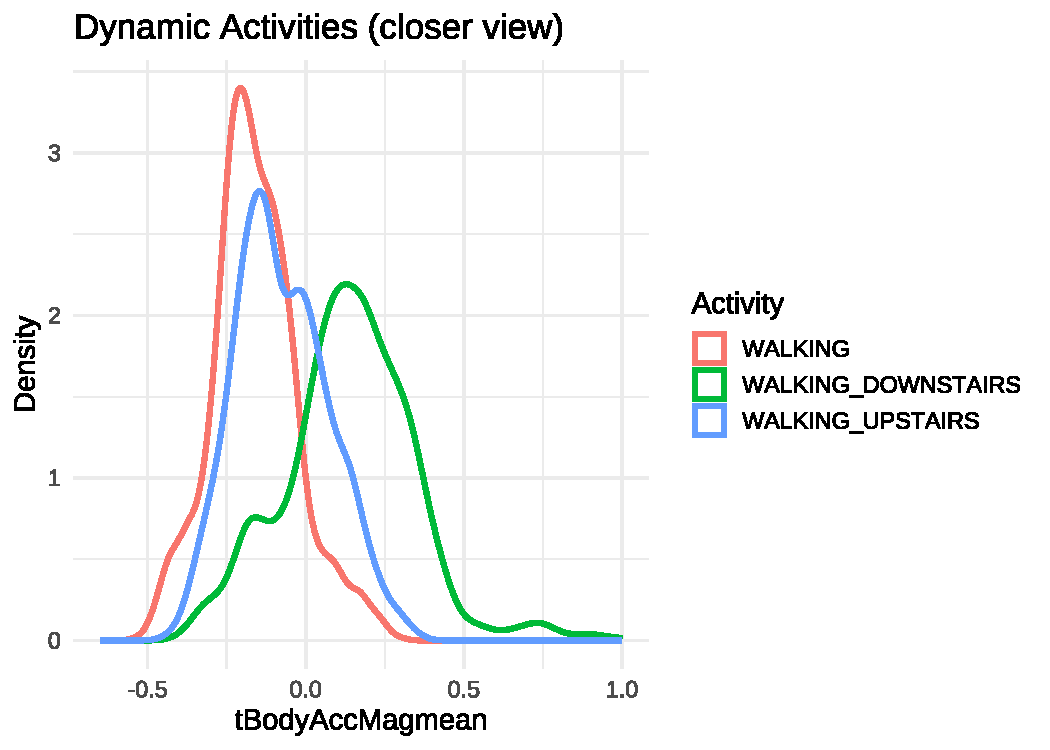
\includegraphics{report_files/figure-latex/unnamed-chunk-13-1.pdf}

\begin{Shaded}
\begin{Highlighting}[]
\FunctionTok{library}\NormalTok{(ggplot2)}
\FunctionTok{library}\NormalTok{(dplyr)}
\end{Highlighting}
\end{Shaded}

\begin{verbatim}
## 
## Attaching package: 'dplyr'
\end{verbatim}

\begin{verbatim}
## The following objects are masked from 'package:stats':
## 
##     filter, lag
\end{verbatim}

\begin{verbatim}
## The following objects are masked from 'package:base':
## 
##     intersect, setdiff, setequal, union
\end{verbatim}

\begin{Shaded}
\begin{Highlighting}[]
\FunctionTok{library}\NormalTok{(gridExtra)}
\end{Highlighting}
\end{Shaded}

\begin{verbatim}
## 
## Attaching package: 'gridExtra'
\end{verbatim}

\begin{verbatim}
## The following object is masked from 'package:dplyr':
## 
##     combine
\end{verbatim}

\begin{Shaded}
\begin{Highlighting}[]
\NormalTok{p1 }\OtherTok{\textless{}{-}}\NormalTok{ train }\SpecialCharTok{\%\textgreater{}\%}
  \FunctionTok{filter}\NormalTok{(Activity }\SpecialCharTok{\%in\%} \FunctionTok{c}\NormalTok{(}\StringTok{"SITTING"}\NormalTok{, }\StringTok{"STANDING"}\NormalTok{, }\StringTok{"LAYING"}\NormalTok{)) }\SpecialCharTok{\%\textgreater{}\%}
  \FunctionTok{ggplot}\NormalTok{(}\FunctionTok{aes}\NormalTok{(}\AttributeTok{x =}\NormalTok{ tBodyAccMagmean, }\AttributeTok{color =}\NormalTok{ Activity)) }\SpecialCharTok{+}
  \FunctionTok{geom\_density}\NormalTok{(}\AttributeTok{size =} \FloatTok{1.2}\NormalTok{) }\SpecialCharTok{+}
  \FunctionTok{labs}\NormalTok{(}
    \AttributeTok{title =} \StringTok{"Static Activities (closer view)"}\NormalTok{,}
    \AttributeTok{x =} \StringTok{"tBodyAccMagmean"}\NormalTok{,}
    \AttributeTok{y =} \StringTok{"Density"}
\NormalTok{  ) }\SpecialCharTok{+}
  \FunctionTok{xlim}\NormalTok{(}\SpecialCharTok{{-}}\FloatTok{1.05}\NormalTok{, }\SpecialCharTok{{-}}\FloatTok{0.1}\NormalTok{) }\SpecialCharTok{+}
  \FunctionTok{ylim}\NormalTok{(}\DecValTok{0}\NormalTok{, }\DecValTok{35}\NormalTok{) }\SpecialCharTok{+}
  \FunctionTok{theme\_minimal}\NormalTok{(}\AttributeTok{base\_size =} \DecValTok{14}\NormalTok{)}
\NormalTok{p1}
\end{Highlighting}
\end{Shaded}

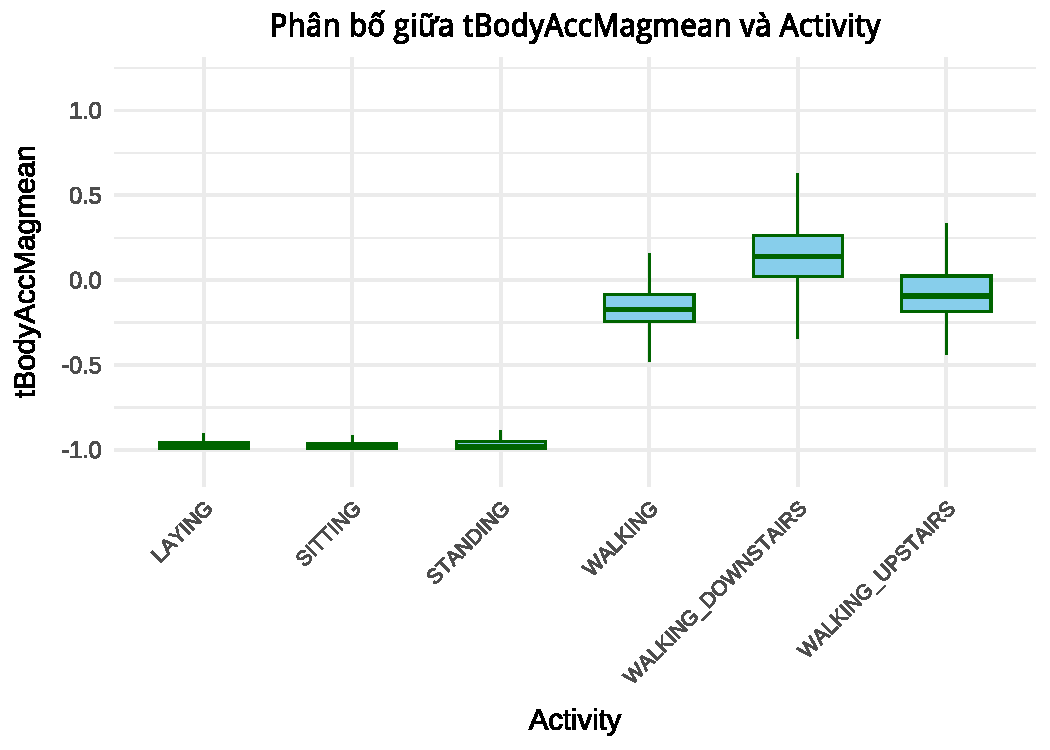
\includegraphics{report_files/figure-latex/unnamed-chunk-14-1.pdf}

\begin{Shaded}
\begin{Highlighting}[]
\NormalTok{p2 }\OtherTok{\textless{}{-}}\NormalTok{ train }\SpecialCharTok{\%\textgreater{}\%}
  \FunctionTok{filter}\NormalTok{(Activity }\SpecialCharTok{\%in\%} \FunctionTok{c}\NormalTok{(}\StringTok{"WALKING"}\NormalTok{, }\StringTok{"WALKING\_DOWNSTAIRS"}\NormalTok{, }\StringTok{"WALKING\_UPSTAIRS"}\NormalTok{)) }\SpecialCharTok{\%\textgreater{}\%}
  \FunctionTok{ggplot}\NormalTok{(}\FunctionTok{aes}\NormalTok{(}\AttributeTok{x =}\NormalTok{ tBodyAccMagmean, }\AttributeTok{color =}\NormalTok{ Activity)) }\SpecialCharTok{+}
  \FunctionTok{geom\_density}\NormalTok{(}\AttributeTok{size =} \FloatTok{1.2}\NormalTok{) }\SpecialCharTok{+}
  \FunctionTok{labs}\NormalTok{(}
    \AttributeTok{title =} \StringTok{"Dynamic Activities (closer view)"}\NormalTok{,}
    \AttributeTok{x =} \StringTok{"tBodyAccMagmean"}\NormalTok{,}
    \AttributeTok{y =} \StringTok{"Density"}
\NormalTok{  ) }\SpecialCharTok{+} \FunctionTok{xlim}\NormalTok{(}\SpecialCharTok{{-}}\FloatTok{0.65}\NormalTok{, }\DecValTok{1}\NormalTok{) }\SpecialCharTok{+}
  \FunctionTok{theme\_minimal}\NormalTok{(}\AttributeTok{base\_size =} \DecValTok{14}\NormalTok{)}

\NormalTok{p2}
\end{Highlighting}
\end{Shaded}

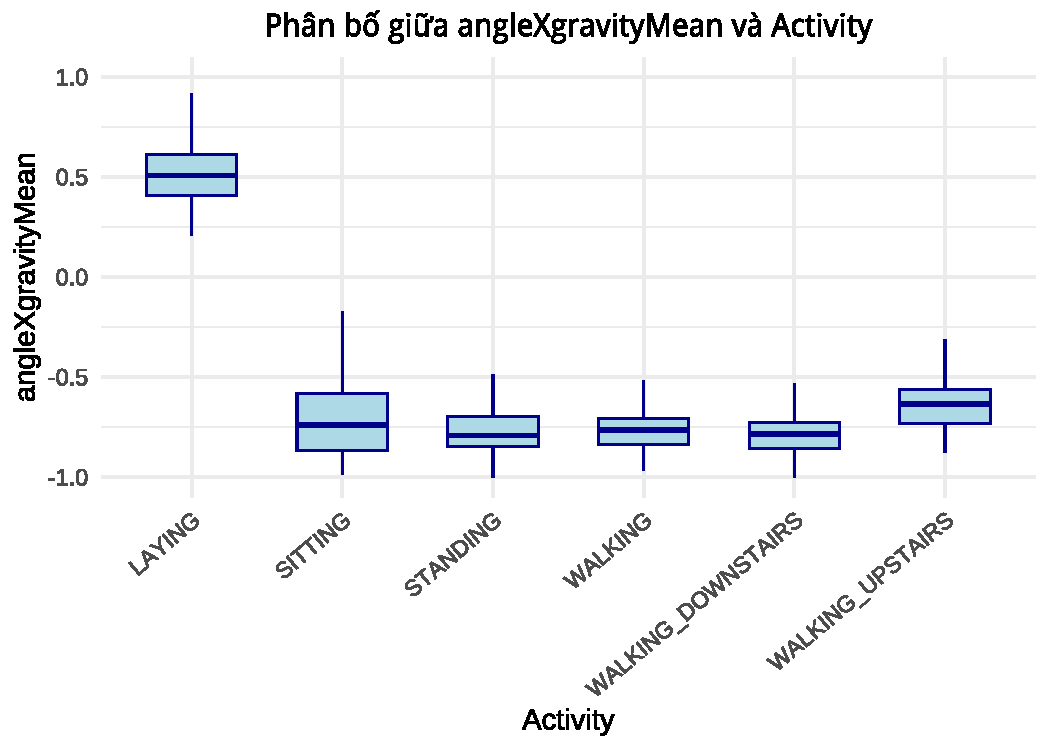
\includegraphics{report_files/figure-latex/unnamed-chunk-15-1.pdf}

\begin{Shaded}
\begin{Highlighting}[]
\FunctionTok{library}\NormalTok{(ggplot2)}

\FunctionTok{ggplot}\NormalTok{(train, }\FunctionTok{aes}\NormalTok{(}\AttributeTok{x =}\NormalTok{ Activity, }\AttributeTok{y =}\NormalTok{ tBodyAccMagmean)) }\SpecialCharTok{+}
  \FunctionTok{geom\_boxplot}\NormalTok{(}
    \AttributeTok{outlier.shape =} \ConstantTok{NA}\NormalTok{,}
    \AttributeTok{fill =} \StringTok{"skyblue"}\NormalTok{,}
    \AttributeTok{color =} \StringTok{"darkgreen"}\NormalTok{,}
    \AttributeTok{width =} \FloatTok{0.6}
\NormalTok{  ) }\SpecialCharTok{+}
  \FunctionTok{labs}\NormalTok{(}
    \AttributeTok{title =} \StringTok{"Phân bố giữa tBodyAccMagmean và Activity"}\NormalTok{,}
    \AttributeTok{y =} \StringTok{"tBodyAccMagmean"}\NormalTok{,}
    \AttributeTok{x =} \StringTok{"Activity"}
\NormalTok{  ) }\SpecialCharTok{+}
  \FunctionTok{coord\_cartesian}\NormalTok{(}\AttributeTok{ylim =} \FunctionTok{c}\NormalTok{(}\SpecialCharTok{{-}}\FloatTok{1.1}\NormalTok{, }\FloatTok{1.2}\NormalTok{)) }\SpecialCharTok{+} 
  \FunctionTok{theme\_minimal}\NormalTok{(}\AttributeTok{base\_size =} \DecValTok{14}\NormalTok{) }\SpecialCharTok{+}
  \FunctionTok{theme}\NormalTok{(}
    \AttributeTok{plot.title =} \FunctionTok{element\_text}\NormalTok{(}\AttributeTok{hjust =} \FloatTok{0.5}\NormalTok{, }\AttributeTok{size =} \DecValTok{15}\NormalTok{, }\AttributeTok{face =} \StringTok{"bold"}\NormalTok{),}
    \AttributeTok{axis.text.x =} \FunctionTok{element\_text}\NormalTok{(}\AttributeTok{angle =} \DecValTok{45}\NormalTok{, }\AttributeTok{hjust =} \DecValTok{1}\NormalTok{, }\AttributeTok{size =} \DecValTok{12}\NormalTok{),}
    \AttributeTok{axis.title.x =} \FunctionTok{element\_text}\NormalTok{(}\AttributeTok{margin =} \FunctionTok{margin}\NormalTok{(}\AttributeTok{t =} \DecValTok{10}\NormalTok{)),}
    \AttributeTok{axis.title.y =} \FunctionTok{element\_text}\NormalTok{(}\AttributeTok{margin =} \FunctionTok{margin}\NormalTok{(}\AttributeTok{r =} \DecValTok{10}\NormalTok{))}
\NormalTok{  )}
\end{Highlighting}
\end{Shaded}

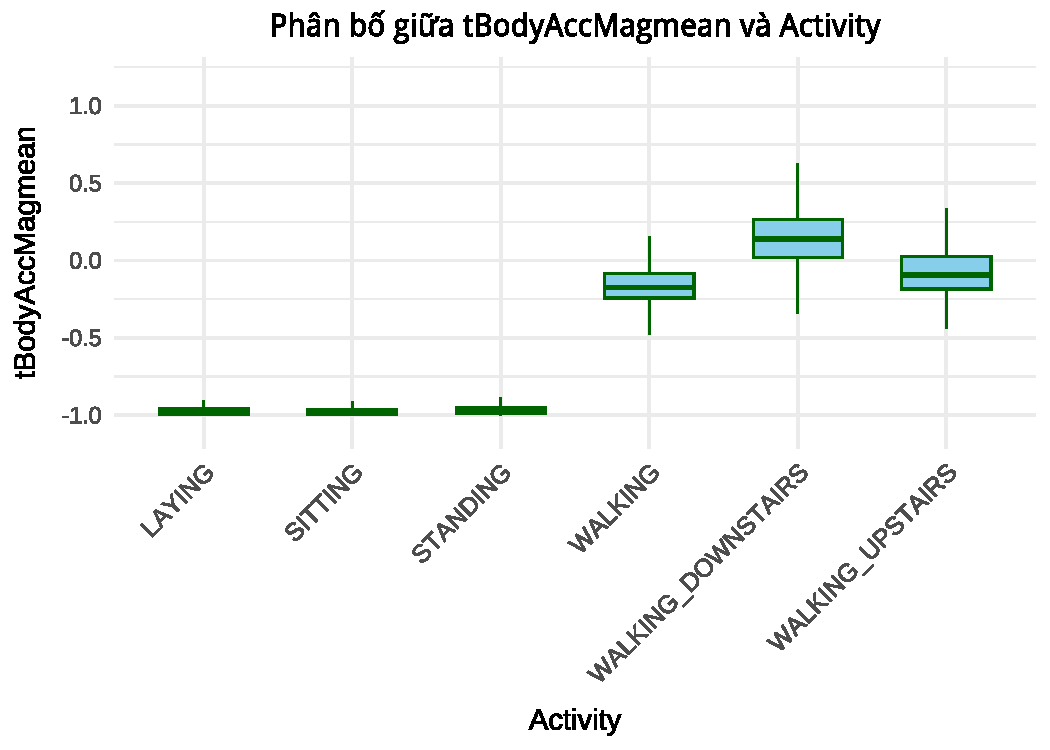
\includegraphics{report_files/figure-latex/unnamed-chunk-16-1.pdf}

\begin{Shaded}
\begin{Highlighting}[]
\FunctionTok{library}\NormalTok{(ggplot2)}

\FunctionTok{ggplot}\NormalTok{(train, }\FunctionTok{aes}\NormalTok{(}\AttributeTok{x =}\NormalTok{ Activity, }\AttributeTok{y =}\NormalTok{ angleXgravityMean)) }\SpecialCharTok{+}
  \FunctionTok{geom\_boxplot}\NormalTok{(}
    \AttributeTok{fill =} \StringTok{"lightblue"}\NormalTok{,}
    \AttributeTok{color =} \StringTok{"darkblue"}\NormalTok{,}
    \AttributeTok{outlier.shape =} \ConstantTok{NA}\NormalTok{,}
    \AttributeTok{width =} \FloatTok{0.6}
\NormalTok{  ) }\SpecialCharTok{+}
  \FunctionTok{labs}\NormalTok{(}
    \AttributeTok{title =} \StringTok{"Phân bố giữa angleXgravityMean và Activity"}\NormalTok{,}
    \AttributeTok{x =} \StringTok{"Activity"}\NormalTok{,}
    \AttributeTok{y =} \StringTok{"angleXgravityMean"}
\NormalTok{  ) }\SpecialCharTok{+}
  \FunctionTok{theme\_minimal}\NormalTok{(}\AttributeTok{base\_size =} \DecValTok{14}\NormalTok{) }\SpecialCharTok{+}
  \FunctionTok{theme}\NormalTok{(}
    \AttributeTok{plot.title =} \FunctionTok{element\_text}\NormalTok{(}\AttributeTok{hjust =} \FloatTok{0.5}\NormalTok{, }\AttributeTok{size =} \DecValTok{15}\NormalTok{, }\AttributeTok{face =} \StringTok{"bold"}\NormalTok{),}
    \AttributeTok{axis.text.x =} \FunctionTok{element\_text}\NormalTok{(}\AttributeTok{angle =} \DecValTok{40}\NormalTok{, }\AttributeTok{hjust =} \DecValTok{1}\NormalTok{, }\AttributeTok{size =} \DecValTok{11}\NormalTok{)}
\NormalTok{  )}
\end{Highlighting}
\end{Shaded}

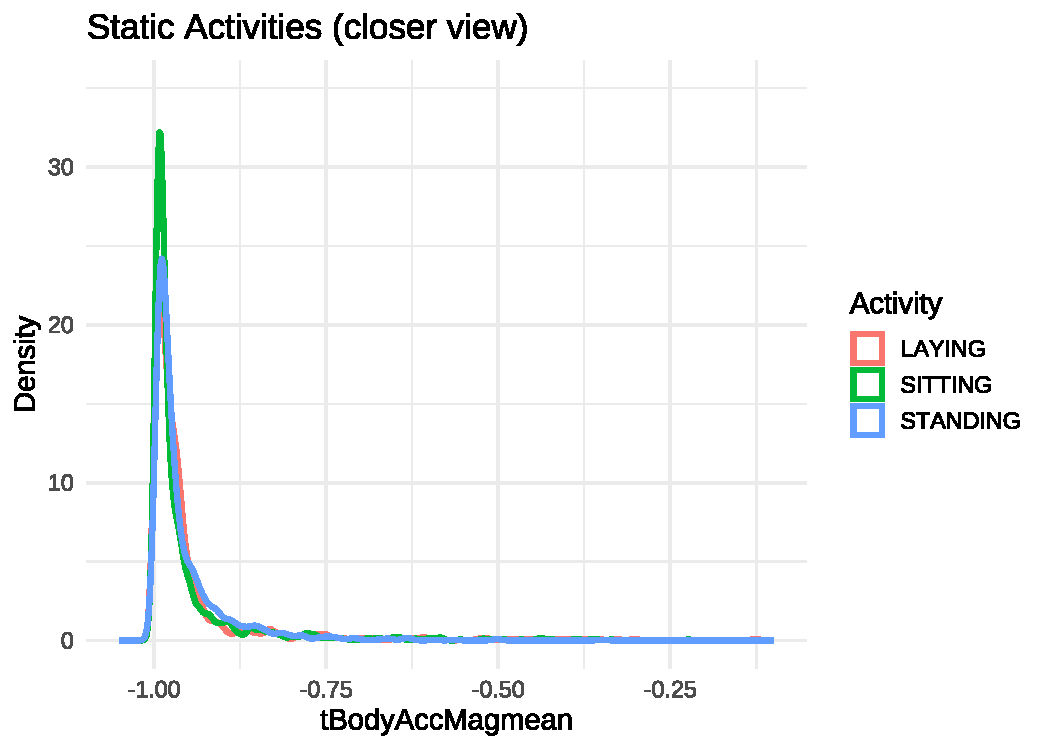
\includegraphics{report_files/figure-latex/unnamed-chunk-17-1.pdf}

\begin{Shaded}
\begin{Highlighting}[]
\FunctionTok{library}\NormalTok{(ggplot2)}

\FunctionTok{ggplot}\NormalTok{(train, }\FunctionTok{aes}\NormalTok{(}\AttributeTok{x =}\NormalTok{ Activity, }\AttributeTok{y =}\NormalTok{ angleYgravityMean)) }\SpecialCharTok{+}
  \FunctionTok{geom\_boxplot}\NormalTok{(}
    \AttributeTok{fill =} \StringTok{"lightblue"}\NormalTok{,}
    \AttributeTok{color =} \StringTok{"darkblue"}\NormalTok{,}
    \AttributeTok{outlier.shape =} \ConstantTok{NA}\NormalTok{,}
    \AttributeTok{width =} \FloatTok{0.6}
\NormalTok{  ) }\SpecialCharTok{+}
  \FunctionTok{labs}\NormalTok{(}
    \AttributeTok{title =} \StringTok{"Phân bố giữa angleYgravityMean và Activity"}\NormalTok{,}
    \AttributeTok{x =} \StringTok{"Activity"}\NormalTok{,}
    \AttributeTok{y =} \StringTok{"angleYgravityMean"}
\NormalTok{  ) }\SpecialCharTok{+}
  \FunctionTok{theme\_minimal}\NormalTok{(}\AttributeTok{base\_size =} \DecValTok{14}\NormalTok{) }\SpecialCharTok{+}
  \FunctionTok{theme}\NormalTok{(}
    \AttributeTok{plot.title =} \FunctionTok{element\_text}\NormalTok{(}\AttributeTok{hjust =} \FloatTok{0.5}\NormalTok{, }\AttributeTok{size =} \DecValTok{15}\NormalTok{, }\AttributeTok{face =} \StringTok{"bold"}\NormalTok{),}
    \AttributeTok{axis.text.x =} \FunctionTok{element\_text}\NormalTok{(}\AttributeTok{angle =} \DecValTok{40}\NormalTok{, }\AttributeTok{hjust =} \DecValTok{1}\NormalTok{, }\AttributeTok{size =} \DecValTok{11}\NormalTok{)}
\NormalTok{  )}
\end{Highlighting}
\end{Shaded}

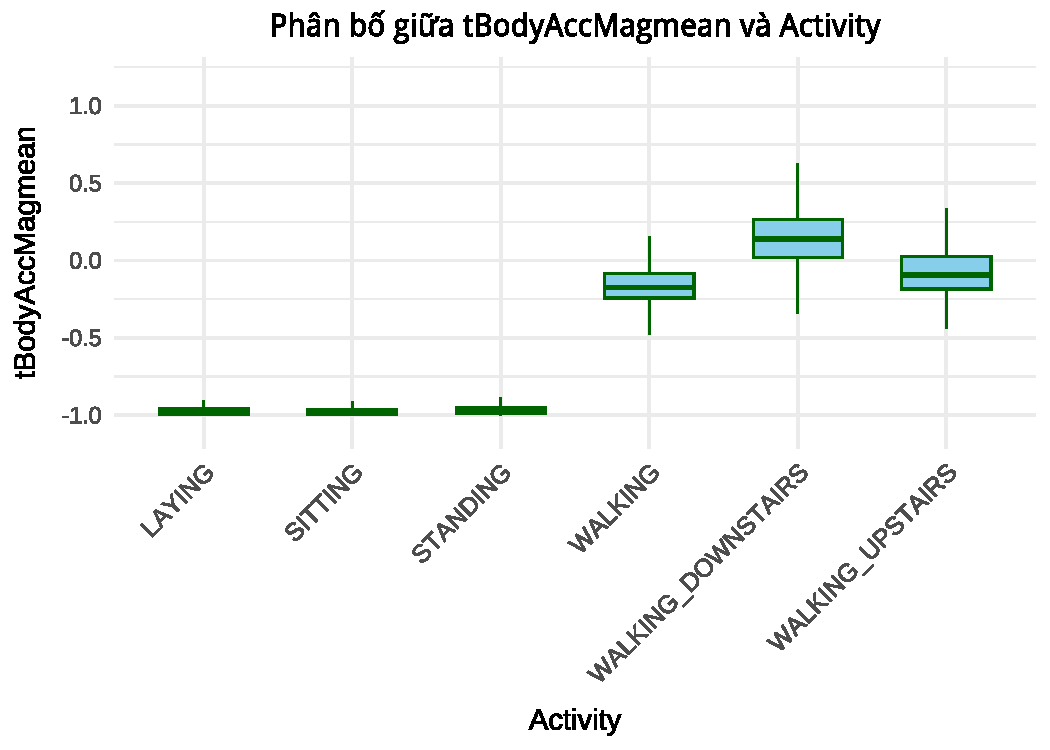
\includegraphics{report_files/figure-latex/unnamed-chunk-18-1.pdf}

\begin{Shaded}
\begin{Highlighting}[]
\NormalTok{subject\_ids }\OtherTok{\textless{}{-}}\NormalTok{ train}\SpecialCharTok{$}\NormalTok{subject}
\NormalTok{activity\_labels }\OtherTok{\textless{}{-}}\NormalTok{ train}\SpecialCharTok{$}\NormalTok{Activity}
\NormalTok{sensor\_data }\OtherTok{\textless{}{-}}\NormalTok{ train[, }\SpecialCharTok{!}\NormalTok{(}\FunctionTok{names}\NormalTok{(train) }\SpecialCharTok{\%in\%} \FunctionTok{c}\NormalTok{(}\StringTok{"Activity"}\NormalTok{, }\StringTok{"subject"}\NormalTok{))]}
\NormalTok{subject\_ids\_test }\OtherTok{\textless{}{-}}\NormalTok{ test}\SpecialCharTok{$}\NormalTok{subject}
\NormalTok{activity\_labels\_test }\OtherTok{\textless{}{-}}\NormalTok{ test}\SpecialCharTok{$}\NormalTok{Activity}
\NormalTok{sensor\_data\_test }\OtherTok{\textless{}{-}}\NormalTok{ test[, }\SpecialCharTok{!}\NormalTok{(}\FunctionTok{names}\NormalTok{(test) }\SpecialCharTok{\%in\%} \FunctionTok{c}\NormalTok{(}\StringTok{"Activity"}\NormalTok{, }\StringTok{"subject"}\NormalTok{))]}

\NormalTok{is\_outlier\_iqr }\OtherTok{\textless{}{-}} \ControlFlowTok{function}\NormalTok{(x) \{}
\NormalTok{  Q1 }\OtherTok{\textless{}{-}} \FunctionTok{quantile}\NormalTok{(x, }\FloatTok{0.25}\NormalTok{, }\AttributeTok{na.rm =} \ConstantTok{TRUE}\NormalTok{)}
\NormalTok{  Q3 }\OtherTok{\textless{}{-}} \FunctionTok{quantile}\NormalTok{(x, }\FloatTok{0.75}\NormalTok{, }\AttributeTok{na.rm =} \ConstantTok{TRUE}\NormalTok{)}
\NormalTok{  IQR\_val }\OtherTok{\textless{}{-}}\NormalTok{ Q3 }\SpecialCharTok{{-}}\NormalTok{ Q1}
\NormalTok{  lower\_bound }\OtherTok{\textless{}{-}}\NormalTok{ Q1 }\SpecialCharTok{{-}} \FloatTok{1.5} \SpecialCharTok{*}\NormalTok{ IQR\_val}
\NormalTok{  upper\_bound }\OtherTok{\textless{}{-}}\NormalTok{ Q3 }\SpecialCharTok{+} \FloatTok{1.5} \SpecialCharTok{*}\NormalTok{ IQR\_val}
\NormalTok{  x }\SpecialCharTok{\textless{}}\NormalTok{ lower\_bound }\SpecialCharTok{|}\NormalTok{ x }\SpecialCharTok{\textgreater{}}\NormalTok{ upper\_bound}
\NormalTok{\}}

\NormalTok{outlier\_matrix }\OtherTok{\textless{}{-}} \FunctionTok{mapply}\NormalTok{(is\_outlier\_iqr, sensor\_data)}

\NormalTok{total\_outlier\_values }\OtherTok{\textless{}{-}} \FunctionTok{sum}\NormalTok{(outlier\_matrix)}
\NormalTok{total\_cells }\OtherTok{\textless{}{-}} \FunctionTok{nrow}\NormalTok{(sensor\_data) }\SpecialCharTok{*} \FunctionTok{ncol}\NormalTok{(sensor\_data)}
\NormalTok{percent\_outlier\_cells }\OtherTok{\textless{}{-}} \FunctionTok{round}\NormalTok{(total\_outlier\_values }\SpecialCharTok{/}\NormalTok{ total\_cells }\SpecialCharTok{*} \DecValTok{100}\NormalTok{, }\DecValTok{2}\NormalTok{)}

\FunctionTok{cat}\NormalTok{(}\StringTok{"Tổng số giá trị outlier:"}\NormalTok{, total\_outlier\_values, }\StringTok{"/"}\NormalTok{, total\_cells, }\StringTok{"}\SpecialCharTok{\textbackslash{}n}\StringTok{"}\NormalTok{)}
\end{Highlighting}
\end{Shaded}

\begin{verbatim}
## Tổng số giá trị outlier: 163682 / 4124472
\end{verbatim}

\begin{Shaded}
\begin{Highlighting}[]
\FunctionTok{cat}\NormalTok{(}\StringTok{"Tỷ lệ giá trị outlier:"}\NormalTok{, percent\_outlier\_cells, }\StringTok{"\%}\SpecialCharTok{\textbackslash{}n}\StringTok{"}\NormalTok{)}
\end{Highlighting}
\end{Shaded}

\begin{verbatim}
## Tỷ lệ giá trị outlier: 3.97 %
\end{verbatim}

\begin{Shaded}
\begin{Highlighting}[]
\NormalTok{cap\_outliers }\OtherTok{\textless{}{-}} \ControlFlowTok{function}\NormalTok{(df, }\AttributeTok{lower =} \FloatTok{0.01}\NormalTok{, }\AttributeTok{upper =} \FloatTok{0.99}\NormalTok{) \{}
  \ControlFlowTok{for}\NormalTok{ (col }\ControlFlowTok{in} \FunctionTok{names}\NormalTok{(df)) \{}
\NormalTok{    q\_low }\OtherTok{\textless{}{-}} \FunctionTok{quantile}\NormalTok{(df[[col]], lower, }\AttributeTok{na.rm =} \ConstantTok{TRUE}\NormalTok{)}
\NormalTok{    q\_high }\OtherTok{\textless{}{-}} \FunctionTok{quantile}\NormalTok{(df[[col]], upper, }\AttributeTok{na.rm =} \ConstantTok{TRUE}\NormalTok{)}
\NormalTok{    df[[col]] }\OtherTok{\textless{}{-}} \FunctionTok{pmin}\NormalTok{(}\FunctionTok{pmax}\NormalTok{(df[[col]], q\_low), q\_high)}
\NormalTok{  \}}
\NormalTok{  df}
\NormalTok{\}}

\NormalTok{sensor\_data\_capped }\OtherTok{\textless{}{-}} \FunctionTok{cap\_outliers}\NormalTok{(sensor\_data)}
\NormalTok{sensor\_data\_test\_capped }\OtherTok{\textless{}{-}} \FunctionTok{cap\_outliers}\NormalTok{(sensor\_data\_test)}

\NormalTok{train\_capped }\OtherTok{\textless{}{-}} \FunctionTok{cbind}\NormalTok{(sensor\_data\_capped, }\AttributeTok{subject =}\NormalTok{ subject\_ids, }\AttributeTok{Activity =}\NormalTok{ activity\_labels)}
\NormalTok{test\_capped }\OtherTok{\textless{}{-}} \FunctionTok{cbind}\NormalTok{(sensor\_data\_test\_capped, }\AttributeTok{subject =}\NormalTok{ subject\_ids\_test, }\AttributeTok{Activity =}\NormalTok{ activity\_labels\_test)}

\FunctionTok{str}\NormalTok{(train\_capped)}
\end{Highlighting}
\end{Shaded}

\begin{verbatim}
## 'data.frame':    7352 obs. of  563 variables:
##  $ tBodyAccmeanX                    : num  0.289 0.278 0.28 0.279 0.277 ...
##  $ tBodyAccmeanY                    : num  -0.0203 -0.0164 -0.0195 -0.0262 -0.0166 ...
##  $ tBodyAccmeanZ                    : num  -0.133 -0.124 -0.113 -0.123 -0.115 ...
##  $ tBodyAccstdX                     : num  -0.995 -0.998 -0.995 -0.996 -0.998 ...
##  $ tBodyAccstdY                     : num  -0.983 -0.975 -0.967 -0.983 -0.981 ...
##  $ tBodyAccstdZ                     : num  -0.914 -0.96 -0.979 -0.991 -0.99 ...
##  $ tBodyAccmadX                     : num  -0.995 -0.999 -0.997 -0.997 -0.998 ...
##  $ tBodyAccmadY                     : num  -0.983 -0.975 -0.964 -0.983 -0.98 ...
##  $ tBodyAccmadZ                     : num  -0.924 -0.958 -0.977 -0.989 -0.99 ...
##  $ tBodyAccmaxX                     : num  -0.935 -0.943 -0.939 -0.939 -0.942 ...
##  $ tBodyAccmaxY                     : num  -0.567 -0.558 -0.558 -0.576 -0.569 ...
##  $ tBodyAccmaxZ                     : num  -0.744 -0.818 -0.818 -0.828 -0.825 ...
##  $ tBodyAccminX                     : num  0.853 0.849 0.844 0.844 0.849 ...
##  $ tBodyAccminY                     : num  0.686 0.686 0.682 0.682 0.683 ...
##  $ tBodyAccminZ                     : num  0.814 0.823 0.839 0.838 0.838 ...
##  $ tBodyAccsma                      : num  -0.966 -0.982 -0.983 -0.986 -0.993 ...
##  $ tBodyAccenergyX                  : num  -1 -1 -1 -1 -1 ...
##  $ tBodyAccenergyY                  : num  -1 -1 -1 -1 -1 ...
##  $ tBodyAccenergyZ                  : num  -0.995 -0.998 -0.999 -1 -1 ...
##  $ tBodyAcciqrX                     : num  -0.994 -0.999 -0.997 -0.997 -0.998 ...
##  $ tBodyAcciqrY                     : num  -0.988 -0.978 -0.965 -0.984 -0.981 ...
##  $ tBodyAcciqrZ                     : num  -0.943 -0.948 -0.975 -0.986 -0.991 ...
##  $ tBodyAccentropyX                 : num  -0.408 -0.715 -0.592 -0.627 -0.787 ...
##  $ tBodyAccentropyY                 : num  -0.679 -0.501 -0.486 -0.851 -0.559 ...
##  $ tBodyAccentropyZ                 : num  -0.602 -0.571 -0.571 -0.866 -0.761 ...
##  $ tBodyAccarCoeffX1                : num  0.5 0.5 0.273 0.0614 0.3133 ...
##  $ tBodyAccarCoeffX2                : num  -0.3591 -0.3295 -0.0863 0.0748 -0.1312 ...
##  $ tBodyAccarCoeffX3                : num  0.36 0.284 0.337 0.198 0.191 ...
##  $ tBodyAccarCoeffX4                : num  -0.0585 0.2846 -0.1647 -0.2643 0.0869 ...
##  $ tBodyAccarCoeffY1                : num  0.2569 0.1157 0.0172 0.0725 0.2576 ...
##  $ tBodyAccarCoeffY2                : num  -0.2248 -0.091 -0.0745 -0.1553 -0.2725 ...
##  $ tBodyAccarCoeffY3                : num  0.264 0.294 0.342 0.323 0.435 ...
##  $ tBodyAccarCoeffY4                : num  -0.0952 -0.2812 -0.3326 -0.1708 -0.3154 ...
##  $ tBodyAccarCoeffZ1                : num  0.279 0.086 0.239 0.295 0.44 ...
##  $ tBodyAccarCoeffZ2                : num  -0.3917 -0.0222 -0.1362 -0.3061 -0.2691 ...
##  $ tBodyAccarCoeffZ3                : num  0.4919 -0.0167 0.1739 0.4821 0.1794 ...
##  $ tBodyAccarCoeffZ4                : num  -0.191 -0.221 -0.299 -0.47 -0.089 ...
##  $ tBodyAcccorrelationXY            : num  0.3763 -0.0134 -0.1247 -0.3057 -0.1558 ...
##  $ tBodyAcccorrelationXZ            : num  0.4351 -0.0727 -0.1811 -0.3627 -0.1898 ...
##  $ tBodyAcccorrelationYZ            : num  0.661 0.579 0.609 0.507 0.599 ...
##  $ tGravityAccmeanX                 : num  0.963 0.967 0.967 0.968 0.968 ...
##  $ tGravityAccmeanY                 : num  -0.141 -0.142 -0.142 -0.144 -0.149 ...
##  $ tGravityAccmeanZ                 : num  0.1154 0.1094 0.1019 0.0999 0.0945 ...
##  $ tGravityAccstdX                  : num  -0.985 -0.997 -0.999 -0.997 -0.998 ...
##  $ tGravityAccstdY                  : num  -0.982 -0.989 -0.993 -0.981 -0.988 ...
##  $ tGravityAccstdZ                  : num  -0.878 -0.932 -0.993 -0.978 -0.979 ...
##  $ tGravityAccmadX                  : num  -0.985 -0.998 -0.999 -0.996 -0.998 ...
##  $ tGravityAccmadY                  : num  -0.984 -0.99 -0.993 -0.981 -0.989 ...
##  $ tGravityAccmadZ                  : num  -0.895 -0.933 -0.993 -0.978 -0.979 ...
##  $ tGravityAccmaxX                  : num  0.892 0.892 0.892 0.894 0.894 ...
##  $ tGravityAccmaxY                  : num  -0.161 -0.161 -0.164 -0.164 -0.167 ...
##  $ tGravityAccmaxZ                  : num  0.1247 0.1226 0.0946 0.0934 0.0917 ...
##  $ tGravityAccminX                  : num  0.977 0.985 0.987 0.987 0.987 ...
##  $ tGravityAccminY                  : num  -0.123 -0.115 -0.115 -0.121 -0.122 ...
##  $ tGravityAccminZ                  : num  0.0565 0.1028 0.1028 0.0958 0.0941 ...
##  $ tGravityAccsma                   : num  -0.375 -0.383 -0.402 -0.4 -0.4 ...
##  $ tGravityAccenergyX               : num  0.899 0.908 0.909 0.911 0.912 ...
##  $ tGravityAccenergyY               : num  -0.971 -0.971 -0.97 -0.969 -0.967 ...
##  $ tGravityAccenergyZ               : num  -0.976 -0.979 -0.982 -0.982 -0.984 ...
##  $ tGravityAcciqrX                  : num  -0.984 -0.999 -1 -0.996 -0.998 ...
##  $ tGravityAcciqrY                  : num  -0.989 -0.99 -0.992 -0.981 -0.991 ...
##  $ tGravityAcciqrZ                  : num  -0.918 -0.942 -0.993 -0.98 -0.98 ...
##  $ tGravityAccentropyX              : num  -1 -1 -1 -1 -1 -1 -1 -1 -1 -1 ...
##  $ tGravityAccentropyY              : num  -1 -1 -1 -1 -1 -1 -1 -1 -1 -1 ...
##  $ tGravityAccentropyZ              : num  0.114 -0.21 -0.927 -0.596 -0.617 ...
##  $ tGravityAccarCoeffX1             : num  -0.59042 -0.41006 0.00223 -0.06493 -0.25727 ...
##  $ tGravityAccarCoeffX2             : num  0.5911 0.4139 0.0371 0.0754 0.2689 ...
##  $ tGravityAccarCoeffX3             : num  -0.5918 -0.4176 -0.0732 -0.0858 -0.2807 ...
##  $ tGravityAccarCoeffX4             : num  0.592 0.421 0.106 0.106 0.293 ...
##  $ tGravityAccarCoeffY1             : num  -0.745 -0.196 -0.329 -0.295 -0.167 ...
##  $ tGravityAccarCoeffY2             : num  0.7209 0.1253 0.2705 0.2283 0.0899 ...
##  $ tGravityAccarCoeffY3             : num  -0.7124 -0.1056 -0.2545 -0.2063 -0.0663 ...
##  $ tGravityAccarCoeffY4             : num  0.7113 0.1091 0.2576 0.2048 0.0671 ...
##  $ tGravityAccarCoeffZ1             : num  -0.969 -0.834 -0.705 -0.385 -0.237 ...
##  $ tGravityAccarCoeffZ2             : num  0.972 0.834 0.714 0.386 0.239 ...
##  $ tGravityAccarCoeffZ3             : num  -0.977 -0.834 -0.723 -0.387 -0.241 ...
##  $ tGravityAccarCoeffZ4             : num  0.978 0.83 0.729 0.385 0.241 ...
##  $ tGravityAcccorrelationXY         : num  0.57 -0.831 -0.181 -0.991 -0.408 ...
##  $ tGravityAcccorrelationXZ         : num  0.439 -0.866 0.338 -0.969 -0.185 ...
##  $ tGravityAcccorrelationYZ         : num  0.987 0.974 0.643 0.984 0.965 ...
##  $ tBodyAccJerkmeanX                : num  0.078 0.074 0.0736 0.0773 0.0734 ...
##  $ tBodyAccJerkmeanY                : num  0.005 0.00577 0.0031 0.02006 0.01912 ...
##  $ tBodyAccJerkmeanZ                : num  -0.06783 0.02938 -0.00905 -0.00986 0.01678 ...
##  $ tBodyAccJerkstdX                 : num  -0.994 -0.996 -0.991 -0.993 -0.996 ...
##  $ tBodyAccJerkstdY                 : num  -0.988 -0.981 -0.981 -0.988 -0.988 ...
##  $ tBodyAccJerkstdZ                 : num  -0.994 -0.992 -0.99 -0.993 -0.992 ...
##  $ tBodyAccJerkmadX                 : num  -0.994 -0.996 -0.991 -0.994 -0.997 ...
##  $ tBodyAccJerkmadY                 : num  -0.986 -0.979 -0.979 -0.986 -0.987 ...
##  $ tBodyAccJerkmadZ                 : num  -0.993 -0.991 -0.987 -0.991 -0.991 ...
##  $ tBodyAccJerkmaxX                 : num  -0.985 -0.995 -0.987 -0.987 -0.997 ...
##  $ tBodyAccJerkmaxY                 : num  -0.992 -0.979 -0.979 -0.992 -0.992 ...
##  $ tBodyAccJerkmaxZ                 : num  -0.993 -0.992 -0.992 -0.99 -0.99 ...
##  $ tBodyAccJerkminX                 : num  0.99 0.993 0.988 0.988 0.994 ...
##  $ tBodyAccJerkminY                 : num  0.992 0.992 0.992 0.993 0.993 ...
##  $ tBodyAccJerkminZ                 : num  0.991 0.989 0.989 0.993 0.986 ...
##  $ tBodyAccJerksma                  : num  -0.994 -0.991 -0.988 -0.993 -0.994 ...
##  $ tBodyAccJerkenergyX              : num  -1 -1 -1 -1 -1 ...
##  $ tBodyAccJerkenergyY              : num  -1 -1 -1 -1 -1 ...
##  $ tBodyAccJerkenergyZ              : num  -1 -1 -1 -1 -1 ...
##   [list output truncated]
\end{verbatim}

\begin{Shaded}
\begin{Highlighting}[]
\FunctionTok{str}\NormalTok{(test\_capped)}
\end{Highlighting}
\end{Shaded}

\begin{verbatim}
## 'data.frame':    2947 obs. of  563 variables:
##  $ tBodyAccmeanX                    : num  0.257 0.286 0.275 0.27 0.275 ...
##  $ tBodyAccmeanY                    : num  -0.0233 -0.0132 -0.0261 -0.0326 -0.0278 ...
##  $ tBodyAccmeanZ                    : num  -0.0147 -0.1191 -0.1182 -0.1175 -0.1295 ...
##  $ tBodyAccstdX                     : num  -0.938 -0.975 -0.994 -0.995 -0.994 ...
##  $ tBodyAccstdY                     : num  -0.92 -0.967 -0.97 -0.973 -0.967 ...
##  $ tBodyAccstdZ                     : num  -0.668 -0.945 -0.963 -0.967 -0.978 ...
##  $ tBodyAccmadX                     : num  -0.953 -0.987 -0.994 -0.995 -0.994 ...
##  $ tBodyAccmadY                     : num  -0.925 -0.968 -0.971 -0.974 -0.966 ...
##  $ tBodyAccmadZ                     : num  -0.674 -0.946 -0.963 -0.969 -0.977 ...
##  $ tBodyAccmaxX                     : num  -0.894 -0.894 -0.939 -0.939 -0.939 ...
##  $ tBodyAccmaxY                     : num  -0.555 -0.555 -0.569 -0.569 -0.561 ...
##  $ tBodyAccmaxZ                     : num  -0.466 -0.806 -0.799 -0.799 -0.826 ...
##  $ tBodyAccminX                     : num  0.717 0.768 0.848 0.848 0.849 ...
##  $ tBodyAccminY                     : num  0.636 0.684 0.668 0.668 0.671 ...
##  $ tBodyAccminZ                     : num  0.789 0.797 0.822 0.822 0.83 ...
##  $ tBodyAccsma                      : num  -0.878 -0.969 -0.977 -0.974 -0.975 ...
##  $ tBodyAccenergyX                  : num  -0.998 -1 -1 -1 -1 ...
##  $ tBodyAccenergyY                  : num  -0.998 -1 -1 -0.999 -0.999 ...
##  $ tBodyAccenergyZ                  : num  -0.934 -0.998 -0.999 -0.999 -0.999 ...
##  $ tBodyAcciqrX                     : num  -0.976 -0.994 -0.993 -0.995 -0.993 ...
##  $ tBodyAcciqrY                     : num  -0.95 -0.974 -0.974 -0.979 -0.967 ...
##  $ tBodyAcciqrZ                     : num  -0.83 -0.951 -0.965 -0.97 -0.976 ...
##  $ tBodyAccentropyX                 : num  -0.168 -0.302 -0.618 -0.75 -0.591 ...
##  $ tBodyAccentropyY                 : num  -0.379 -0.348 -0.695 -0.827 -0.74 ...
##  $ tBodyAccentropyZ                 : num  0.246 -0.405 -0.537 -0.554 -0.799 ...
##  $ tBodyAccarCoeffX1                : num  0.521 0.507 0.242 0.175 0.116 ...
##  $ tBodyAccarCoeffX2                : num  -0.3435 -0.1565 -0.115 -0.0513 -0.0289 ...
##  $ tBodyAccarCoeffX3                : num  0.4823 0.0407 0.0327 0.0342 -0.0328 ...
##  $ tBodyAccarCoeffX4                : num  -0.0455 0.273 0.1924 0.1536 0.2943 ...
##  $ tBodyAccarCoeffY1                : num  0.21196 0.19757 -0.01194 0.03077 0.00063 ...
##  $ tBodyAccarCoeffY2                : num  -0.1349 -0.1946 -0.0634 -0.1293 -0.0453 ...
##  $ tBodyAccarCoeffY3                : num  0.131 0.411 0.471 0.446 0.168 ...
##  $ tBodyAccarCoeffY4                : num  -0.0142 -0.3405 -0.5074 -0.4195 -0.0682 ...
##  $ tBodyAccarCoeffZ1                : num  -0.106 0.0776 0.1885 0.2715 0.0744 ...
##  $ tBodyAccarCoeffZ2                : num  0.0735 -0.084 -0.2316 -0.2258 0.0271 ...
##  $ tBodyAccarCoeffZ3                : num  -0.1715 0.0353 0.5482 0.4164 -0.1459 ...
##  $ tBodyAccarCoeffZ4                : num  0.0401 -0.0101 -0.5507 -0.2864 -0.0502 ...
##  $ tBodyAcccorrelationXY            : num  0.077 -0.105 0.3057 -0.0638 0.2352 ...
##  $ tBodyAcccorrelationXZ            : num  -0.491 -0.429 -0.324 -0.167 0.29 ...
##  $ tBodyAcccorrelationYZ            : num  -0.709 0.399 0.28 0.545 0.458 ...
##  $ tGravityAccmeanX                 : num  0.936 0.927 0.93 0.929 0.927 ...
##  $ tGravityAccmeanY                 : num  -0.283 -0.289 -0.288 -0.293 -0.303 ...
##  $ tGravityAccmeanZ                 : num  0.115 0.153 0.146 0.143 0.138 ...
##  $ tGravityAccstdX                  : num  -0.925 -0.989 -0.996 -0.993 -0.996 ...
##  $ tGravityAccstdY                  : num  -0.937 -0.984 -0.988 -0.97 -0.971 ...
##  $ tGravityAccstdZ                  : num  -0.603 -0.965 -0.982 -0.992 -0.968 ...
##  $ tGravityAccmadX                  : num  -0.93 -0.989 -0.996 -0.993 -0.996 ...
##  $ tGravityAccmadY                  : num  -0.938 -0.983 -0.989 -0.971 -0.971 ...
##  $ tGravityAccmadZ                  : num  -0.607 -0.965 -0.98 -0.993 -0.969 ...
##  $ tGravityAccmaxX                  : num  0.906 0.856 0.856 0.856 0.854 ...
##  $ tGravityAccmaxY                  : num  -0.279 -0.305 -0.305 -0.305 -0.313 ...
##  $ tGravityAccmaxZ                  : num  0.153 0.153 0.139 0.136 0.134 ...
##  $ tGravityAccminX                  : num  0.944 0.944 0.949 0.947 0.946 ...
##  $ tGravityAccminY                  : num  -0.262 -0.262 -0.262 -0.273 -0.279 ...
##  $ tGravityAccminZ                  : num  -0.0762 0.149 0.145 0.1421 0.1309 ...
##  $ tGravityAccsma                   : num  -0.0178 0.0577 0.0406 0.0461 0.0554 ...
##  $ tGravityAccenergyX               : num  0.829 0.806 0.812 0.809 0.804 ...
##  $ tGravityAccenergyY               : num  -0.865 -0.858 -0.86 -0.854 -0.843 ...
##  $ tGravityAccenergyZ               : num  -0.968 -0.957 -0.961 -0.963 -0.965 ...
##  $ tGravityAcciqrX                  : num  -0.95 -0.988 -0.996 -0.992 -0.996 ...
##  $ tGravityAcciqrY                  : num  -0.946 -0.982 -0.99 -0.973 -0.972 ...
##  $ tGravityAcciqrZ                  : num  -0.76 -0.971 -0.979 -0.996 -0.969 ...
##  $ tGravityAccentropyX              : num  -0.425 -0.729 -0.823 -0.823 -0.83 ...
##  $ tGravityAccentropyY              : num  -1 -1 -1 -1 -1 -1 -1 -1 -1 -1 ...
##  $ tGravityAccentropyZ              : num  0.219 -0.465 -0.53 -0.7 -0.302 ...
##  $ tGravityAccarCoeffX1             : num  -0.43 -0.51 -0.295 -0.343 -0.482 ...
##  $ tGravityAccarCoeffX2             : num  0.431 0.525 0.305 0.359 0.539 ...
##  $ tGravityAccarCoeffX3             : num  -0.432 -0.54 -0.315 -0.375 -0.596 ...
##  $ tGravityAccarCoeffX4             : num  0.433 0.554 0.326 0.392 0.655 ...
##  $ tGravityAccarCoeffY1             : num  -0.795 -0.746 -0.232 -0.233 -0.493 ...
##  $ tGravityAccarCoeffY2             : num  0.781 0.733 0.169 0.176 0.463 ...
##  $ tGravityAccarCoeffY3             : num  -0.78 -0.737 -0.155 -0.169 -0.465 ...
##  $ tGravityAccarCoeffY4             : num  0.785 0.749 0.164 0.185 0.483 ...
##  $ tGravityAccarCoeffZ1             : num  -0.958 -0.845 -0.429 -0.297 -0.536 ...
##  $ tGravityAccarCoeffZ2             : num  0.962 0.869 0.44 0.304 0.544 ...
##  $ tGravityAccarCoeffZ3             : num  -0.964 -0.893 -0.451 -0.311 -0.553 ...
##  $ tGravityAccarCoeffZ4             : num  0.966 0.913 0.458 0.315 0.559 ...
##  $ tGravityAcccorrelationXY         : num  0.981 0.945 0.548 0.986 0.997 ...
##  $ tGravityAcccorrelationXZ         : num  -0.996 -0.911 -0.335 0.653 0.916 ...
##  $ tGravityAcccorrelationYZ         : num  -0.96 -0.739 0.59 0.747 0.929 ...
##  $ tBodyAccJerkmeanX                : num  0.072 0.0702 0.0694 0.0749 0.0784 ...
##  $ tBodyAccJerkmeanY                : num  0.04575 -0.01788 -0.00491 0.03227 0.02228 ...
##  $ tBodyAccJerkmeanZ                : num  -0.10604 -0.00172 -0.01367 0.01214 0.00275 ...
##  $ tBodyAccJerkstdX                 : num  -0.907 -0.949 -0.991 -0.991 -0.992 ...
##  $ tBodyAccJerkstdY                 : num  -0.938 -0.973 -0.971 -0.973 -0.979 ...
##  $ tBodyAccJerkstdZ                 : num  -0.936 -0.978 -0.973 -0.976 -0.987 ...
##  $ tBodyAccJerkmadX                 : num  -0.916 -0.969 -0.991 -0.99 -0.991 ...
##  $ tBodyAccJerkmadY                 : num  -0.937 -0.974 -0.973 -0.973 -0.977 ...
##  $ tBodyAccJerkmadZ                 : num  -0.949 -0.979 -0.975 -0.978 -0.985 ...
##  $ tBodyAccJerkmaxX                 : num  -0.903 -0.915 -0.992 -0.992 -0.994 ...
##  $ tBodyAccJerkmaxY                 : num  -0.95 -0.981 -0.975 -0.975 -0.986 ...
##  $ tBodyAccJerkmaxZ                 : num  -0.891 -0.978 -0.962 -0.962 -0.986 ...
##  $ tBodyAccJerkminX                 : num  0.898 0.898 0.994 0.994 0.994 ...
##  $ tBodyAccJerkminY                 : num  0.95 0.968 0.976 0.976 0.98 ...
##  $ tBodyAccJerkminZ                 : num  0.946 0.966 0.966 0.97 0.985 ...
##  $ tBodyAccJerksma                  : num  -0.931 -0.974 -0.982 -0.983 -0.987 ...
##  $ tBodyAccJerkenergyX              : num  -0.995 -0.998 -1 -1 -1 ...
##  $ tBodyAccJerkenergyY              : num  -0.997 -0.999 -0.999 -0.999 -1 ...
##  $ tBodyAccJerkenergyZ              : num  -0.997 -0.999 -0.999 -0.999 -1 ...
##   [list output truncated]
\end{verbatim}

\begin{Shaded}
\begin{Highlighting}[]
\FunctionTok{library}\NormalTok{(umap)}
\FunctionTok{library}\NormalTok{(ggplot2)}
\FunctionTok{library}\NormalTok{(gridExtra)}

\NormalTok{perform\_umap\_grid }\OtherTok{\textless{}{-}} \ControlFlowTok{function}\NormalTok{(X\_data, y\_data,}
                              \AttributeTok{neighbors\_list =} \FunctionTok{c}\NormalTok{(}\DecValTok{5}\NormalTok{, }\DecValTok{15}\NormalTok{, }\DecValTok{30}\NormalTok{),}
                              \AttributeTok{min\_dist\_list =} \FunctionTok{c}\NormalTok{(}\FloatTok{0.001}\NormalTok{, }\FloatTok{0.01}\NormalTok{, }\FloatTok{0.1}\NormalTok{)) \{}
\NormalTok{  plots }\OtherTok{\textless{}{-}} \FunctionTok{list}\NormalTok{()}
\NormalTok{  index }\OtherTok{\textless{}{-}} \DecValTok{1}
  
  \ControlFlowTok{for}\NormalTok{ (n }\ControlFlowTok{in}\NormalTok{ neighbors\_list) \{}
    \ControlFlowTok{for}\NormalTok{ (d }\ControlFlowTok{in}\NormalTok{ min\_dist\_list) \{}
\NormalTok{      config }\OtherTok{\textless{}{-}}\NormalTok{ umap.defaults}
\NormalTok{      config}\SpecialCharTok{$}\NormalTok{n\_neighbors }\OtherTok{\textless{}{-}}\NormalTok{ n}
\NormalTok{      config}\SpecialCharTok{$}\NormalTok{min\_dist }\OtherTok{\textless{}{-}}\NormalTok{ d}
\NormalTok{      config}\SpecialCharTok{$}\NormalTok{n\_components }\OtherTok{\textless{}{-}} \DecValTok{2}
      
\NormalTok{      umap\_result }\OtherTok{\textless{}{-}} \FunctionTok{umap}\NormalTok{(X\_data, }\AttributeTok{config =}\NormalTok{ config)}
\NormalTok{      df }\OtherTok{\textless{}{-}} \FunctionTok{as.data.frame}\NormalTok{(umap\_result}\SpecialCharTok{$}\NormalTok{layout)}
      \FunctionTok{colnames}\NormalTok{(df) }\OtherTok{\textless{}{-}} \FunctionTok{c}\NormalTok{(}\StringTok{"x"}\NormalTok{, }\StringTok{"y"}\NormalTok{)}
\NormalTok{      df}\SpecialCharTok{$}\NormalTok{label }\OtherTok{\textless{}{-}}\NormalTok{ y\_data}
      
\NormalTok{      p }\OtherTok{\textless{}{-}} \FunctionTok{ggplot}\NormalTok{(df, }\FunctionTok{aes}\NormalTok{(}\AttributeTok{x =}\NormalTok{ x, }\AttributeTok{y =}\NormalTok{ y, }\AttributeTok{color =}\NormalTok{ label)) }\SpecialCharTok{+}
        \FunctionTok{geom\_point}\NormalTok{(}\AttributeTok{size =} \FloatTok{0.6}\NormalTok{, }\AttributeTok{alpha =} \FloatTok{0.6}\NormalTok{) }\SpecialCharTok{+}
        \FunctionTok{scale\_color\_brewer}\NormalTok{(}\AttributeTok{palette =} \StringTok{"Set1"}\NormalTok{) }\SpecialCharTok{+}
        \FunctionTok{theme\_minimal}\NormalTok{(}\AttributeTok{base\_size =} \DecValTok{10}\NormalTok{) }\SpecialCharTok{+}
        \FunctionTok{labs}\NormalTok{(}\AttributeTok{title =} \FunctionTok{paste}\NormalTok{(}\StringTok{"n ="}\NormalTok{, n, }\StringTok{", dist ="}\NormalTok{, d), }\AttributeTok{x =} \ConstantTok{NULL}\NormalTok{, }\AttributeTok{y =} \ConstantTok{NULL}\NormalTok{) }\SpecialCharTok{+}
        \FunctionTok{theme}\NormalTok{(}\AttributeTok{legend.position =} \StringTok{"none"}\NormalTok{,}
              \AttributeTok{plot.title =} \FunctionTok{element\_text}\NormalTok{(}\AttributeTok{size =} \DecValTok{10}\NormalTok{, }\AttributeTok{hjust =} \FloatTok{0.5}\NormalTok{))}
      
\NormalTok{      plots[[index]] }\OtherTok{\textless{}{-}}\NormalTok{ p}
\NormalTok{      index }\OtherTok{\textless{}{-}}\NormalTok{ index }\SpecialCharTok{+} \DecValTok{1}
\NormalTok{    \}}
\NormalTok{  \}}
  
  \FunctionTok{do.call}\NormalTok{(grid.arrange, }\FunctionTok{c}\NormalTok{(plots, }\AttributeTok{ncol =} \FunctionTok{length}\NormalTok{(min\_dist\_list)))}
\NormalTok{\}}

\FunctionTok{perform\_umap\_grid}\NormalTok{(}
  \AttributeTok{X\_data =}\NormalTok{ sensor\_data\_capped,}
  \AttributeTok{y\_data =}\NormalTok{ train}\SpecialCharTok{$}\NormalTok{Activity,}
  \AttributeTok{neighbors\_list =} \FunctionTok{c}\NormalTok{(}\DecValTok{5}\NormalTok{, }\DecValTok{15}\NormalTok{, }\DecValTok{30}\NormalTok{),}
  \AttributeTok{min\_dist\_list =} \FunctionTok{c}\NormalTok{(}\FloatTok{0.001}\NormalTok{, }\FloatTok{0.01}\NormalTok{, }\FloatTok{0.1}\NormalTok{)}
\NormalTok{)}
\end{Highlighting}
\end{Shaded}

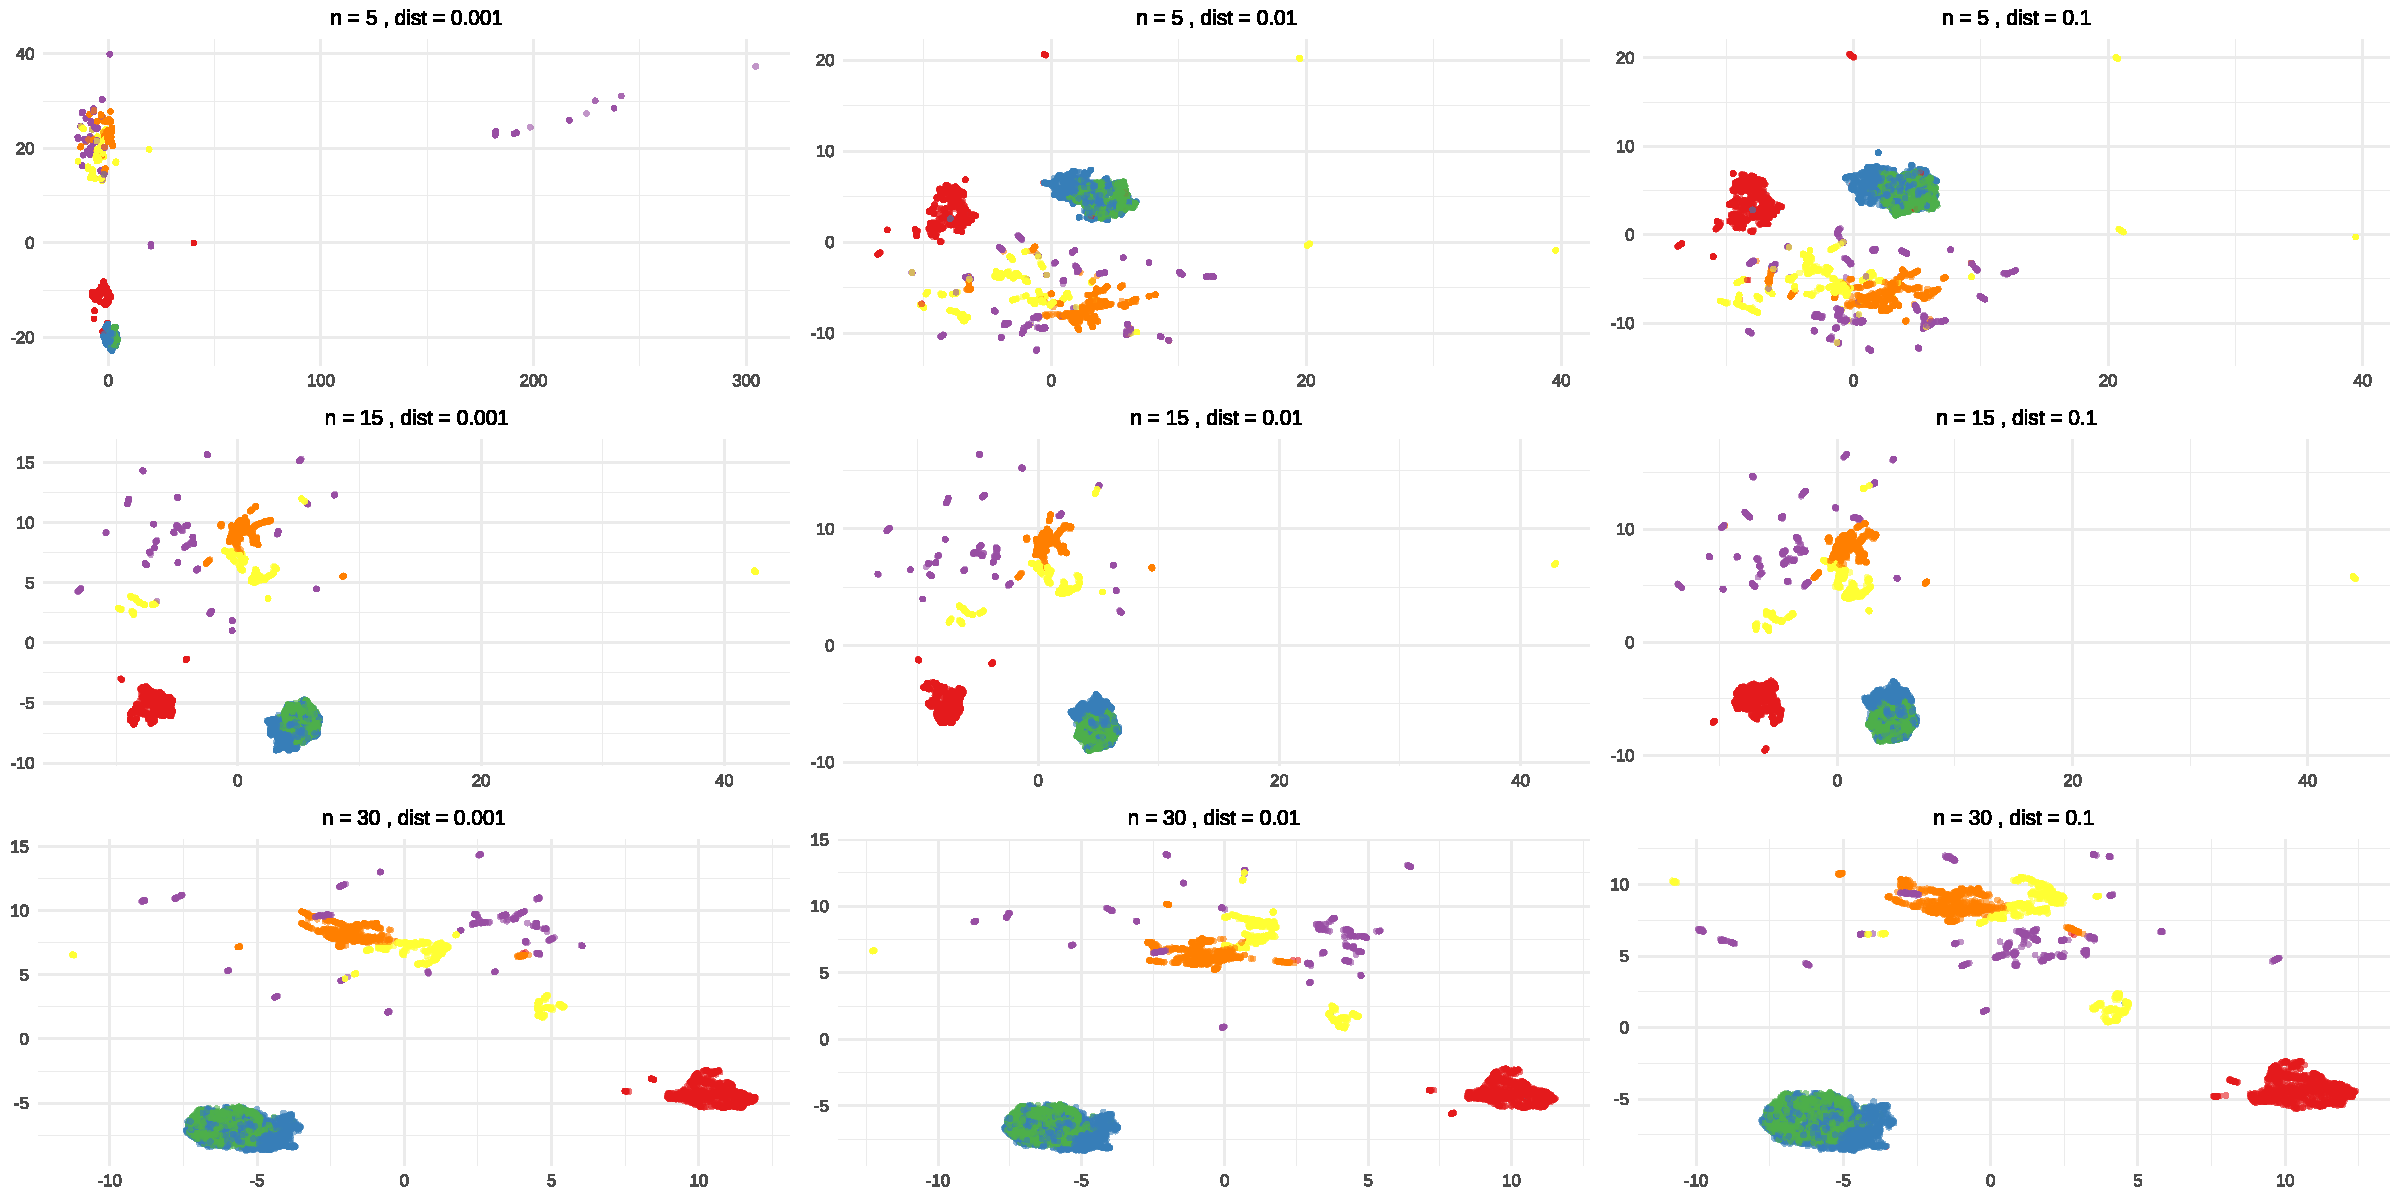
\includegraphics{report_files/figure-latex/unnamed-chunk-21-1.pdf}

\begin{Shaded}
\begin{Highlighting}[]
\FunctionTok{library}\NormalTok{(umap)}
\FunctionTok{library}\NormalTok{(ggplot2)}

\NormalTok{config }\OtherTok{\textless{}{-}}\NormalTok{ umap.defaults}
\NormalTok{config}\SpecialCharTok{$}\NormalTok{n\_neighbors }\OtherTok{\textless{}{-}} \DecValTok{30}
\NormalTok{config}\SpecialCharTok{$}\NormalTok{min\_dist }\OtherTok{\textless{}{-}} \FloatTok{0.1}
\NormalTok{config}\SpecialCharTok{$}\NormalTok{n\_components }\OtherTok{\textless{}{-}} \DecValTok{2}

\NormalTok{umap\_result }\OtherTok{\textless{}{-}} \FunctionTok{umap}\NormalTok{(sensor\_data\_capped, }\AttributeTok{config =}\NormalTok{ config)}

\NormalTok{umap\_df }\OtherTok{\textless{}{-}} \FunctionTok{as.data.frame}\NormalTok{(umap\_result}\SpecialCharTok{$}\NormalTok{layout)}
\FunctionTok{colnames}\NormalTok{(umap\_df) }\OtherTok{\textless{}{-}} \FunctionTok{c}\NormalTok{(}\StringTok{"UMAP\_1"}\NormalTok{, }\StringTok{"UMAP\_2"}\NormalTok{)}
\NormalTok{umap\_df}\SpecialCharTok{$}\NormalTok{Activity }\OtherTok{\textless{}{-}}\NormalTok{ train}\SpecialCharTok{$}\NormalTok{Activity}

\FunctionTok{ggplot}\NormalTok{(umap\_df, }\FunctionTok{aes}\NormalTok{(}\AttributeTok{x =}\NormalTok{ UMAP\_1, }\AttributeTok{y =}\NormalTok{ UMAP\_2, }\AttributeTok{color =}\NormalTok{ Activity)) }\SpecialCharTok{+}
  \FunctionTok{geom\_point}\NormalTok{(}\AttributeTok{size =} \FloatTok{0.7}\NormalTok{, }\AttributeTok{alpha =} \FloatTok{0.6}\NormalTok{) }\SpecialCharTok{+}
  \FunctionTok{scale\_color\_brewer}\NormalTok{(}\AttributeTok{palette =} \StringTok{"Set1"}\NormalTok{) }\SpecialCharTok{+}
  \FunctionTok{theme\_minimal}\NormalTok{(}\AttributeTok{base\_size =} \DecValTok{14}\NormalTok{) }\SpecialCharTok{+}
  \FunctionTok{labs}\NormalTok{(}
    \AttributeTok{title =} \StringTok{"UMAP (n\_neighbors = 30, min\_dist = 0.01)"}\NormalTok{,}
    \AttributeTok{x =} \StringTok{"UMAP 1"}\NormalTok{, }\AttributeTok{y =} \StringTok{"UMAP 2"}
\NormalTok{  )}
\end{Highlighting}
\end{Shaded}

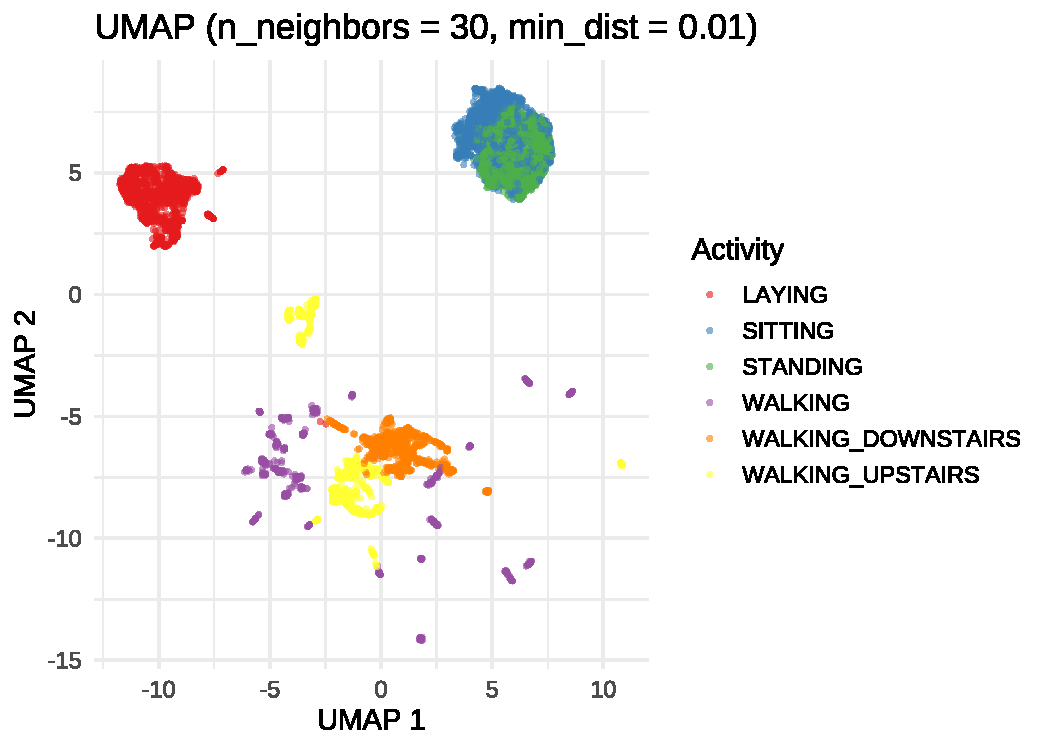
\includegraphics{report_files/figure-latex/unnamed-chunk-22-1.pdf}

\begin{Shaded}
\begin{Highlighting}[]
\NormalTok{X\_train }\OtherTok{\textless{}{-}}\NormalTok{ train\_capped[, }\SpecialCharTok{!}\NormalTok{(}\FunctionTok{names}\NormalTok{(train\_capped) }\SpecialCharTok{\%in\%} \FunctionTok{c}\NormalTok{(}\StringTok{"subject"}\NormalTok{, }\StringTok{"Activity"}\NormalTok{))]}
\NormalTok{y\_train }\OtherTok{\textless{}{-}}\NormalTok{ train\_capped}\SpecialCharTok{$}\NormalTok{Activity}

\NormalTok{X\_test }\OtherTok{\textless{}{-}}\NormalTok{ test\_capped[, }\SpecialCharTok{!}\NormalTok{(}\FunctionTok{names}\NormalTok{(test\_capped) }\SpecialCharTok{\%in\%} \FunctionTok{c}\NormalTok{(}\StringTok{"subject"}\NormalTok{, }\StringTok{"Activity"}\NormalTok{))]}
\NormalTok{y\_test }\OtherTok{\textless{}{-}}\NormalTok{ test\_capped}\SpecialCharTok{$}\NormalTok{Activity}

\FunctionTok{dim}\NormalTok{(X\_train)}
\end{Highlighting}
\end{Shaded}

\begin{verbatim}
## [1] 7352  561
\end{verbatim}

\begin{Shaded}
\begin{Highlighting}[]
\FunctionTok{length}\NormalTok{(y\_train)}
\end{Highlighting}
\end{Shaded}

\begin{verbatim}
## [1] 7352
\end{verbatim}

\begin{Shaded}
\begin{Highlighting}[]
\FunctionTok{dim}\NormalTok{(X\_test)}
\end{Highlighting}
\end{Shaded}

\begin{verbatim}
## [1] 2947  561
\end{verbatim}

\begin{Shaded}
\begin{Highlighting}[]
\FunctionTok{length}\NormalTok{(y\_test)}
\end{Highlighting}
\end{Shaded}

\begin{verbatim}
## [1] 2947
\end{verbatim}

\begin{Shaded}
\begin{Highlighting}[]
\FunctionTok{head}\NormalTok{(train)}
\end{Highlighting}
\end{Shaded}

\begin{verbatim}
##   tBodyAccmeanX tBodyAccmeanY tBodyAccmeanZ tBodyAccstdX tBodyAccstdY
## 1     0.2885845   -0.02029417    -0.1329051   -0.9952786   -0.9831106
## 2     0.2784188   -0.01641057    -0.1235202   -0.9982453   -0.9753002
## 3     0.2796531   -0.01946716    -0.1134617   -0.9953796   -0.9671870
## 4     0.2791739   -0.02620065    -0.1232826   -0.9960915   -0.9834027
## 5     0.2766288   -0.01656965    -0.1153619   -0.9981386   -0.9808173
## 6     0.2771988   -0.01009785    -0.1051373   -0.9973350   -0.9904868
##   tBodyAccstdZ tBodyAccmadX tBodyAccmadY tBodyAccmadZ tBodyAccmaxX tBodyAccmaxY
## 1   -0.9135264   -0.9951121   -0.9831846   -0.9235270   -0.9347238   -0.5673781
## 2   -0.9603220   -0.9988072   -0.9749144   -0.9576862   -0.9430675   -0.5578513
## 3   -0.9789440   -0.9965199   -0.9636684   -0.9774686   -0.9386916   -0.5578513
## 4   -0.9906751   -0.9970995   -0.9827498   -0.9893025   -0.9386916   -0.5761589
## 5   -0.9904816   -0.9983211   -0.9796719   -0.9904411   -0.9424691   -0.5691738
## 6   -0.9954200   -0.9976274   -0.9902177   -0.9955489   -0.9424691   -0.5656839
##   tBodyAccmaxZ tBodyAccminX tBodyAccminY tBodyAccminZ tBodyAccsma
## 1   -0.7444125    0.8529474    0.6858446    0.8142628  -0.9655228
## 2   -0.8184087    0.8493079    0.6858446    0.8226368  -0.9819301
## 3   -0.8184087    0.8436090    0.6824009    0.8393442  -0.9834778
## 4   -0.8297115    0.8436090    0.6824009    0.8378693  -0.9860933
## 5   -0.8247053    0.8490951    0.6832498    0.8378693  -0.9926531
## 6   -0.8227661    0.8490951    0.6955857    0.8459216  -0.9939277
##   tBodyAccenergyX tBodyAccenergyY tBodyAccenergyZ tBodyAcciqrX tBodyAcciqrY
## 1      -0.9999446      -0.9998630      -0.9946122   -0.9942308   -0.9876139
## 2      -0.9999913      -0.9997884      -0.9984054   -0.9991504   -0.9778655
## 3      -0.9999691      -0.9996599      -0.9994695   -0.9971301   -0.9648099
## 4      -0.9999755      -0.9997360      -0.9995037   -0.9971804   -0.9837991
## 5      -0.9999906      -0.9998559      -0.9997566   -0.9980043   -0.9812319
## 6      -0.9999855      -0.9998570      -0.9999174   -0.9975839   -0.9918468
##   tBodyAcciqrZ tBodyAccentropyX tBodyAccentropyY tBodyAccentropyZ
## 1   -0.9432200       -0.4077471       -0.6793375       -0.6021219
## 2   -0.9482248       -0.7148917       -0.5009300       -0.5709791
## 3   -0.9746750       -0.5922351       -0.4858207       -0.5709791
## 4   -0.9860068       -0.6274463       -0.8509300       -0.9118716
## 5   -0.9913247       -0.7865525       -0.5594769       -0.7614338
## 6   -0.9954136       -0.7518691       -0.4547725       -0.5508815
##   tBodyAccarCoeffX1 tBodyAccarCoeffX2 tBodyAccarCoeffX3 tBodyAccarCoeffX4
## 1        0.92929351       -0.85301114         0.3599098       -0.05852638
## 2        0.61162716       -0.32954862         0.2842132        0.28459454
## 3        0.27302484       -0.08630870         0.3372015       -0.16473870
## 4        0.06143571        0.07483956         0.1982040       -0.26430733
## 5        0.31327553       -0.13120773         0.1911608        0.08690362
## 6        0.39005211       -0.18227238         0.1587515        0.18731256
##   tBodyAccarCoeffY1 tBodyAccarCoeffY2 tBodyAccarCoeffY3 tBodyAccarCoeffY4
## 1        0.25689154       -0.22484763         0.2641057       -0.09524563
## 2        0.11570542       -0.09096253         0.2943104       -0.28121057
## 3        0.01715013       -0.07450693         0.3422563       -0.33256448
## 4        0.07254524       -0.15531983         0.3231540       -0.17081296
## 5        0.25761535       -0.27250466         0.4347278       -0.31537507
## 6        0.25995104       -0.24322958         0.4217361       -0.41846005
##   tBodyAccarCoeffZ1 tBodyAccarCoeffZ2 tBodyAccarCoeffZ3 tBodyAccarCoeffZ4
## 1        0.27885143       -0.46508457        0.49193596       -0.19088356
## 2        0.08598843       -0.02215269       -0.01665654       -0.22064350
## 3        0.23928053       -0.13620359        0.17386318       -0.29949278
## 4        0.29493839       -0.30608099        0.48214783       -0.47012871
## 5        0.43974437       -0.26906895        0.17941419       -0.08895195
## 6        0.55846137       -0.21834364        0.16513807        0.08092016
##   tBodyAcccorrelationXY tBodyAcccorrelationXZ tBodyAcccorrelationYZ
## 1            0.37631389            0.43512919             0.6607903
## 2           -0.01342866           -0.07269189             0.5793817
## 3           -0.12469839           -0.18110479             0.6089001
## 4           -0.30569299           -0.36265405             0.5074589
## 5           -0.15580432           -0.18976271             0.5992130
## 6           -0.20997915           -0.15106365             0.1804244
##   tGravityAccmeanX tGravityAccmeanY tGravityAccmeanZ tGravityAccstdX
## 1        0.9633961       -0.1408397       0.11537494      -0.9852497
## 2        0.9665611       -0.1415513       0.10937881      -0.9974113
## 3        0.9668781       -0.1420098       0.10188392      -0.9995740
## 4        0.9676152       -0.1439765       0.09985014      -0.9966456
## 5        0.9682244       -0.1487502       0.09448590      -0.9984293
## 6        0.9679482       -0.1482100       0.09190972      -0.9989793
##   tGravityAccstdY tGravityAccstdZ tGravityAccmadX tGravityAccmadY
## 1      -0.9817084      -0.8776250      -0.9850014      -0.9844162
## 2      -0.9894474      -0.9316387      -0.9978836      -0.9896137
## 3      -0.9928658      -0.9929172      -0.9996353      -0.9926049
## 4      -0.9813928      -0.9784764      -0.9964569      -0.9809618
## 5      -0.9880982      -0.9787449      -0.9984112      -0.9886539
## 6      -0.9867539      -0.9973064      -0.9990540      -0.9865839
##   tGravityAccmadZ tGravityAccmaxX tGravityAccmaxY tGravityAccmaxZ
## 1      -0.8946774       0.8920545      -0.1612655      0.12465977
## 2      -0.9332404       0.8920603      -0.1613426      0.12258573
## 3      -0.9929343       0.8924006      -0.1637112      0.09456584
## 4      -0.9784558       0.8938171      -0.1637112      0.09342467
## 5      -0.9789355       0.8938171      -0.1667862      0.09168239
## 6      -0.9974188       0.8936834      -0.1669704      0.08334712
##   tGravityAccminX tGravityAccminY tGravityAccminZ tGravityAccsma
## 1       0.9774363      -0.1232134      0.05648273     -0.3754260
## 2       0.9845201      -0.1148933      0.10276411     -0.3834296
## 3       0.9867701      -0.1148933      0.10276411     -0.4016016
## 4       0.9868210      -0.1213358      0.09575265     -0.4002781
## 5       0.9874335      -0.1218336      0.09405935     -0.4004765
## 6       0.9877218      -0.1218336      0.09405935     -0.4093585
##   tGravityAccenergyX tGravityAccenergyY tGravityAccenergyZ tGravityAcciqrX
## 1          0.8994686         -0.9709052         -0.9755104      -0.9843254
## 2          0.9078289         -0.9705828         -0.9785004      -0.9991884
## 3          0.9086678         -0.9703681         -0.9816723      -0.9996790
## 4          0.9106207         -0.9693997         -0.9824196      -0.9959764
## 5          0.9122347         -0.9670511         -0.9843626      -0.9983182
## 6          0.9115026         -0.9673206         -0.9852754      -0.9993483
##   tGravityAcciqrY tGravityAcciqrZ tGravityAccentropyX tGravityAccentropyY
## 1      -0.9888491      -0.9177426                  -1                  -1
## 2      -0.9900285      -0.9416854                  -1                  -1
## 3      -0.9921044      -0.9926186                  -1                  -1
## 4      -0.9806634      -0.9797787                  -1                  -1
## 5      -0.9906113      -0.9804125                  -1                  -1
## 6      -0.9865648      -0.9977279                  -1                  -1
##   tGravityAccentropyZ tGravityAccarCoeffX1 tGravityAccarCoeffX2
## 1           0.1138061         -0.590425000           0.59114630
## 2          -0.2104936         -0.410055520           0.41385634
## 3          -0.9267763          0.002234132           0.02748069
## 4          -0.5961008         -0.064934877           0.07542720
## 5          -0.6165782         -0.257266810           0.26891819
## 6          -1.0000000         -0.302224840           0.37903209
##   tGravityAccarCoeffX3 tGravityAccarCoeffX4 tGravityAccarCoeffY1
## 1          -0.59177346           0.59246928           -0.7454488
## 2          -0.41756716           0.42132499           -0.1963593
## 3          -0.05672816           0.08553324           -0.3290230
## 4          -0.08582296           0.09620771           -0.2950360
## 5          -0.28066510           0.29261602           -0.1666931
## 6          -0.45722246           0.53679840           -0.1981248
##   tGravityAccarCoeffY2 tGravityAccarCoeffY3 tGravityAccarCoeffY4
## 1           0.72086167           -0.7123724            0.7113000
## 2           0.12534464           -0.1055677            0.1090901
## 3           0.27050025           -0.2544902            0.2575976
## 4           0.22830973           -0.2062812            0.2048009
## 5           0.08994272           -0.0663267            0.0671311
## 6           0.12718522           -0.1075539            0.1113645
##   tGravityAccarCoeffZ1 tGravityAccarCoeffZ2 tGravityAccarCoeffZ3
## 1           -0.9951116            0.9956749           -0.9956676
## 2           -0.8338821            0.8342711           -0.8341844
## 3           -0.7050392            0.7143920           -0.7232989
## 4           -0.3854102            0.3863727           -0.3871199
## 5           -0.2374745            0.2392680           -0.2410121
## 6           -0.1579059            0.1753748           -0.1927680
##   tGravityAccarCoeffZ4 tGravityAcccorrelationXY tGravityAcccorrelationXZ
## 1            0.9916527                0.5702216                0.4390273
## 2            0.8304639               -0.8312839               -0.8657111
## 3            0.7287554               -0.1810899                0.3379359
## 4            0.3852631               -0.9913087               -0.9688214
## 5            0.2405685               -0.4083304               -0.1848401
## 6            0.2079647               -0.5639509                0.4664707
##   tGravityAcccorrelationYZ tBodyAccJerkmeanX tBodyAccJerkmeanY
## 1                0.9869131        0.07799634       0.005000803
## 2                0.9743856        0.07400671       0.005771104
## 3                0.6434170        0.07363596       0.003104037
## 4                0.9842555        0.07732061       0.020057642
## 5                0.9647965        0.07344436       0.019121574
## 6                0.4430971        0.07793244       0.018684046
##   tBodyAccJerkmeanZ tBodyAccJerkstdX tBodyAccJerkstdY tBodyAccJerkstdZ
## 1      -0.067830808       -0.9935191       -0.9883600       -0.9935750
## 2       0.029376633       -0.9955481       -0.9810636       -0.9918457
## 3      -0.009045631       -0.9907428       -0.9809556       -0.9896866
## 4      -0.009864772       -0.9926974       -0.9875527       -0.9934976
## 5       0.016779979       -0.9964202       -0.9883587       -0.9924549
## 6       0.009344434       -0.9948136       -0.9887145       -0.9922663
##   tBodyAccJerkmadX tBodyAccJerkmadY tBodyAccJerkmadZ tBodyAccJerkmaxX
## 1       -0.9944876       -0.9862066       -0.9928183       -0.9851801
## 2       -0.9956320       -0.9789380       -0.9912766       -0.9945447
## 3       -0.9909329       -0.9793002       -0.9872381       -0.9870770
## 4       -0.9942660       -0.9857170       -0.9914832       -0.9870770
## 5       -0.9965974       -0.9865370       -0.9906864       -0.9969933
## 6       -0.9952418       -0.9868467       -0.9910667       -0.9941054
##   tBodyAccJerkmaxY tBodyAccJerkmaxZ tBodyAccJerkminX tBodyAccJerkminY
## 1       -0.9919942       -0.9931189        0.9898347        0.9919569
## 2       -0.9790682       -0.9922574        0.9925771        0.9918084
## 3       -0.9790682       -0.9922574        0.9883902        0.9918084
## 4       -0.9917862       -0.9897689        0.9883902        0.9925438
## 5       -0.9918178       -0.9897689        0.9943032        0.9925438
## 6       -0.9918178       -0.9926493        0.9943032        0.9933463
##   tBodyAccJerkminZ tBodyAccJerksma tBodyAccJerkenergyX tBodyAccJerkenergyY
## 1        0.9905192      -0.9935220          -0.9999349          -0.9998204
## 2        0.9885391      -0.9913937          -0.9999597          -0.9996396
## 3        0.9885391      -0.9881477          -0.9998942          -0.9996364
## 4        0.9932176      -0.9928683          -0.9999236          -0.9998029
## 5        0.9856091      -0.9938320          -0.9999692          -0.9998203
## 6        0.9856091      -0.9934730          -0.9999512          -0.9998278
##   tBodyAccJerkenergyZ tBodyAccJerkiqrX tBodyAccJerkiqrY tBodyAccJerkiqrZ
## 1          -0.9998785       -0.9943640       -0.9860249       -0.9892336
## 2          -0.9998454       -0.9938627       -0.9794351       -0.9933838
## 3          -0.9997950       -0.9878457       -0.9801445       -0.9819108
## 4          -0.9998829       -0.9946780       -0.9870330       -0.9888963
## 5          -0.9998599       -0.9958878       -0.9865242       -0.9905717
## 6          -0.9998560       -0.9952809       -0.9873590       -0.9895520
##   tBodyAccJerkentropyX tBodyAccJerkentropyY tBodyAccJerkentropyZ
## 1           -0.8199492           -0.7930464           -0.8888529
## 2           -0.8750964           -0.6553621           -0.7673809
## 3           -0.7536287           -0.6732736           -0.7471068
## 4           -0.8208042           -0.7549682           -0.8252786
## 5           -0.8507439           -0.7462578           -0.7969596
## 6           -0.7787178           -0.7549682           -0.7908859
##   tBodyAccJerkarCoeffX1 tBodyAccJerkarCoeffX2 tBodyAccJerkarCoeffX3
## 1             1.0000000           -0.22074703             0.6368308
## 2             0.4896622            0.07099708             0.3627145
## 3             0.2652248            0.18839474             0.4645835
## 4             0.1228930            0.27641881             0.4574450
## 5             0.2409042            0.13491152             0.2969029
## 6             0.2806858            0.10044972             0.2597405
##   tBodyAccJerkarCoeffX4 tBodyAccJerkarCoeffY1 tBodyAccJerkarCoeffY2
## 1             0.3876436            0.24140146          -0.052252848
## 2             0.5273034            0.14939565           0.062925097
## 3             0.3717179            0.08266488          -0.004621675
## 4             0.1934143            0.10240466          -0.099103220
## 5             0.2871847            0.31897047          -0.143364120
## 6             0.2019468            0.35057743          -0.077269461
##   tBodyAccJerkarCoeffY3 tBodyAccJerkarCoeffY4 tBodyAccJerkarCoeffZ1
## 1             0.2641772             0.3734395             0.3417775
## 2             0.3704934             0.4135481             0.1222157
## 3             0.3274702             0.4376232             0.2578909
## 4             0.1946788             0.4842436             0.3576571
## 5             0.4774545             0.4179662             0.3895371
## 6             0.5626646             0.3519760             0.3686890
##   tBodyAccJerkarCoeffZ2 tBodyAccJerkarCoeffZ3 tBodyAccJerkarCoeffZ4
## 1           -0.56979119             0.2653988            -0.4778749
## 2            0.18061304             0.0474240             0.1665727
## 3            0.07002964             0.1869730             0.2467997
## 4           -0.18703248             0.2980687             0.4518696
## 5           -0.03030909             0.1632612             0.1801889
## 6            0.04338534             0.1473115             0.2991720
##   tBodyAccJerkcorrelationXY tBodyAccJerkcorrelationXZ tBodyAccJerkcorrelationYZ
## 1                -0.3853005                0.03364394               -0.12651082
## 2                -0.2087722                0.08410380               -0.26855390
## 3                -0.1201047               -0.11002563               -0.03995275
## 4                -0.1274952               -0.08327836                0.45705983
## 5                -0.2728836                0.10306475                0.06472931
## 6                -0.3746109                0.04182570               -0.11178209
##   tBodyGyromeanX tBodyGyromeanY tBodyGyromeanZ tBodyGyrostdX tBodyGyrostdY
## 1   -0.006100849    -0.03136479     0.10772540    -0.9853103    -0.9766234
## 2   -0.016111620    -0.08389378     0.10058429    -0.9831200    -0.9890458
## 3   -0.031698294    -0.10233542     0.09612688    -0.9762921    -0.9935518
## 4   -0.043409983    -0.09138618     0.08553770    -0.9913848    -0.9924073
## 5   -0.033960416    -0.07470803     0.07739203    -0.9851836    -0.9923781
## 6   -0.028775508    -0.07039311     0.07901214    -0.9851808    -0.9921175
##   tBodyGyrostdZ tBodyGyromadX tBodyGyromadY tBodyGyromadZ tBodyGyromaxX
## 1    -0.9922053    -0.9845863    -0.9763526    -0.9923616    -0.8670437
## 2    -0.9891212    -0.9868904    -0.9890380    -0.9891846    -0.8649038
## 3    -0.9863787    -0.9749215    -0.9941221    -0.9857862    -0.8649038
## 4    -0.9875542    -0.9915889    -0.9931421    -0.9895849    -0.8853204
## 5    -0.9874019    -0.9869437    -0.9925425    -0.9881628    -0.8701541
## 6    -0.9830768    -0.9857856    -0.9922687    -0.9827049    -0.8701541
##   tBodyGyromaxY tBodyGyromaxZ tBodyGyrominX tBodyGyrominY tBodyGyrominZ
## 1    -0.9337860    -0.7475662     0.8473080     0.9148953     0.8308405
## 2    -0.9535605    -0.7458700     0.8337211     0.9081096     0.8289350
## 3    -0.9590491    -0.7432771     0.8337211     0.9057528     0.8289350
## 4    -0.9566563    -0.7432771     0.8341640     0.9057528     0.8266338
## 5    -0.9533597    -0.7497799     0.8390906     0.9111845     0.8213744
## 6    -0.9533597    -0.7463994     0.8398080     0.9111845     0.8188267
##   tBodyGyrosma tBodyGyroenergyX tBodyGyroenergyY tBodyGyroenergyZ tBodyGyroiqrX
## 1   -0.9671843       -0.9995783       -0.9993543       -0.9997634    -0.9834381
## 2   -0.9806131       -0.9997558       -0.9998973       -0.9998224    -0.9928328
## 3   -0.9762803       -0.9996934       -0.9998283       -0.9998216    -0.9723536
## 4   -0.9822957       -0.9997929       -0.9999023       -0.9998773    -0.9910313
## 5   -0.9852620       -0.9998495       -0.9999519       -0.9998443    -0.9898132
## 6   -0.9852143       -0.9998740       -0.9999466       -0.9997780    -0.9853373
##   tBodyGyroiqrY tBodyGyroiqrZ tBodyGyroentropyX tBodyGyroentropyY
## 1    -0.9786140    -0.9929656       0.082631682         0.2022676
## 2    -0.9893447    -0.9902402       0.007469356        -0.5311566
## 3    -0.9951443    -0.9868311      -0.260942670        -1.0000000
## 4    -0.9941653    -0.9945820      -0.930551140        -0.8266180
## 5    -0.9933367    -0.9911546      -0.628860990        -0.4678076
## 6    -0.9929940    -0.9837056      -0.363801070        -0.3705079
##   tBodyGyroentropyZ tBodyGyroarCoeffX1 tBodyGyroarCoeffX2 tBodyGyroarCoeffX3
## 1        -0.1687567         0.09632324        -0.27498511         0.49864419
## 2        -0.1774446        -0.38768063         0.17913763         0.21078900
## 3        -0.2483707        -0.43715568         0.23898137         0.14523773
## 4        -0.5434217        -0.16588549        -0.01288054         0.32005501
## 5        -0.6508521        -0.21269027         0.00211118         0.38809860
## 6        -0.4621260        -0.40282673         0.24203652         0.05913935
##   tBodyGyroarCoeffX4 tBodyGyroarCoeffY1 tBodyGyroarCoeffY2 tBodyGyroarCoeffY3
## 1        -0.22031685         1.00000000        -0.97297139         0.31665451
## 2        -0.14025958        -0.04703181        -0.06494907         0.11768661
## 3        -0.11391720         0.03231156        -0.12787926         0.11492426
## 4        -0.16511393         0.04455323        -0.12519331         0.07832123
## 5        -0.23327097        -0.16322090         0.18645965        -0.43491617
## 6         0.03028356        -0.11969243         0.15061703        -0.38093733
##   tBodyGyroarCoeffY4 tBodyGyroarCoeffZ1 tBodyGyroarCoeffZ2 tBodyGyroarCoeffZ3
## 1         0.37572641         0.72339919         -0.7711120          0.6902132
## 2         0.08169129         0.04236404         -0.1499284          0.2926189
## 3         0.12539829         0.11209205         -0.1656450          0.1345544
## 4         0.17702758         0.19340165         -0.2071888          0.1124575
## 5         0.65013677         0.23995007         -0.3395292          0.1325371
## 6         0.57330854         0.10377464         -0.2276797          0.1382413
##   tBodyGyroarCoeffZ4 tBodyGyrocorrelationXY tBodyGyrocorrelationXZ
## 1         -0.3318310             0.70958377             0.13487336
## 2         -0.1494293             0.04672124            -0.25692940
## 3          0.1843490            -0.01012957             0.04331158
## 4          0.2020919             0.21019413             0.14110084
## 5          0.4732514            -0.14200070             0.48441885
## 6          0.3461755            -0.44810249             0.64501358
##   tBodyGyrocorrelationYZ tBodyGyroJerkmeanX tBodyGyroJerkmeanY
## 1              0.3010995        -0.09916740        -0.05551737
## 2              0.1693948        -0.11050283        -0.04481873
## 3             -0.3506461        -0.10848567        -0.04241031
## 4             -0.7253011        -0.09116989        -0.03633262
## 5             -0.7245575        -0.09077010        -0.03763253
## 6             -0.7459792        -0.09424758        -0.04335526
##   tBodyGyroJerkmeanZ tBodyGyroJerkstdX tBodyGyroJerkstdY tBodyGyroJerkstdZ
## 1        -0.06198580        -0.9921107        -0.9925193        -0.9920553
## 2        -0.05924282        -0.9898726        -0.9972926        -0.9938510
## 3        -0.05582883        -0.9884618        -0.9956321        -0.9915318
## 4        -0.06046466        -0.9911194        -0.9966410        -0.9933289
## 5        -0.05828932        -0.9913545        -0.9964730        -0.9945110
## 6        -0.04193600        -0.9916216        -0.9960147        -0.9930906
##   tBodyGyroJerkmadX tBodyGyroJerkmadY tBodyGyroJerkmadZ tBodyGyroJerkmaxX
## 1        -0.9921648        -0.9949416        -0.9926190        -0.9901558
## 2        -0.9898762        -0.9974917        -0.9937783        -0.9919469
## 3        -0.9878680        -0.9957250        -0.9915963        -0.9933590
## 4        -0.9912405        -0.9969579        -0.9940195        -0.9936763
## 5        -0.9928823        -0.9965406        -0.9943830        -0.9798455
## 6        -0.9930196        -0.9960382        -0.9926340        -0.9798455
##   tBodyGyroJerkmaxY tBodyGyroJerkmaxZ tBodyGyroJerkminX tBodyGyroJerkminY
## 1        -0.9867428        -0.9920416         0.9944288         0.9917558
## 2        -0.9977171        -0.9949208         0.9904860         0.9971222
## 3        -0.9938002        -0.9889631         0.9892905         0.9971222
## 4        -0.9938002        -0.9889631         0.9892905         0.9981303
## 5        -0.9975093        -0.9934198         0.9936848         0.9974531
## 6        -0.9975093        -0.9934198         0.9938443         0.9974531
##   tBodyGyroJerkminZ tBodyGyroJerksma tBodyGyroJerkenergyX tBodyGyroJerkenergyY
## 1         0.9893519       -0.9944534           -0.9999375           -0.9999535
## 2         0.9945031       -0.9952984           -0.9999077           -0.9999897
## 3         0.9941426       -0.9934149           -0.9998871           -0.9999798
## 4         0.9941426       -0.9954961           -0.9999251           -0.9999862
## 5         0.9965279       -0.9958778           -0.9999280           -0.9999852
## 6         0.9965279       -0.9952321           -0.9999316           -0.9999824
##   tBodyGyroJerkenergyZ tBodyGyroJerkiqrX tBodyGyroJerkiqrY tBodyGyroJerkiqrZ
## 1           -0.9999229        -0.9922997        -0.9969389        -0.9922430
## 2           -0.9999459        -0.9907418        -0.9973013        -0.9938078
## 3           -0.9999158        -0.9871304        -0.9954278        -0.9927755
## 4           -0.9999396        -0.9909086        -0.9970785        -0.9954046
## 5           -0.9999535        -0.9945132        -0.9967177        -0.9939689
## 6           -0.9999362        -0.9937336        -0.9961224        -0.9919696
##   tBodyGyroJerkentropyX tBodyGyroJerkentropyY tBodyGyroJerkentropyZ
## 1            -0.5898510            -0.6884590            -0.5721069
## 2            -0.6009445            -0.7482472            -0.6089321
## 3            -0.5436348            -0.6729573            -0.5884104
## 4            -0.5620311            -0.7313321            -0.6614345
## 5            -0.6177378            -0.6830932            -0.6329272
## 6            -0.6278635            -0.6805905            -0.5418971
##   tBodyGyroJerkarCoeffX1 tBodyGyroJerkarCoeffX2 tBodyGyroJerkarCoeffX3
## 1            0.292376340            -0.36199802             0.40554269
## 2           -0.193307570            -0.06740646             0.18561907
## 3           -0.241150980            -0.01137728             0.11613363
## 4            0.009894985            -0.13757147             0.12596517
## 5           -0.025678521            -0.18813916             0.23094957
## 6           -0.265496090             0.05580409            -0.04563533
##   tBodyGyroJerkarCoeffX4 tBodyGyroJerkarCoeffY1 tBodyGyroJerkarCoeffY2
## 1            -0.03900695             0.98928381           -0.414560480
## 2             0.04152181             0.07235255           -0.035377727
## 3             0.08962988             0.09598603            0.009604215
## 4             0.31611970             0.09433295            0.026171325
## 5             0.20025838            -0.14940028            0.271977090
## 6             0.23627625            -0.12219895            0.268114140
##   tBodyGyroJerkarCoeffY3 tBodyGyroJerkarCoeffY4 tBodyGyroJerkarCoeffZ1
## 1             0.39160251            0.282250870              0.9272698
## 2             0.17760636            0.027498054              0.1827027
## 3             0.09512614            0.252887040              0.1816489
## 4             0.06966099            0.246653200              0.2573553
## 5            -0.27151547           -0.009937466              0.2351285
## 6            -0.19369246           -0.005319577              0.2034059
##   tBodyGyroJerkarCoeffZ2 tBodyGyroJerkarCoeffZ3 tBodyGyroJerkarCoeffZ4
## 1             -0.5723700             0.69161920            0.468289820
## 2             -0.1674574             0.25325103            0.132333860
## 3             -0.1693084             0.13200906            0.008197317
## 4             -0.1368088             0.08731557            0.149095580
## 5             -0.3409670            -0.08571288            0.163956800
## 6             -0.2967479             0.06993358           -0.012261880
##   tBodyGyroJerkcorrelationXY tBodyGyroJerkcorrelationXZ
## 1                -0.13107697                -0.08715969
## 2                 0.29385535                -0.01807517
## 3                 0.19332856                 0.07371786
## 4                 0.19665725                 0.14045188
## 5                 0.12059038                 0.10748923
## 6                 0.01791207                 0.18667289
##   tBodyGyroJerkcorrelationYZ tBodyAccMagmean tBodyAccMagstd tBodyAccMagmad
## 1                  0.3362475      -0.9594339     -0.9505515     -0.9579929
## 2                 -0.3433368      -0.9792892     -0.9760571     -0.9782473
## 3                 -0.3148578      -0.9837031     -0.9880196     -0.9883268
## 4                 -0.3058977      -0.9865418     -0.9864213     -0.9864305
## 5                 -0.2825893      -0.9928271     -0.9912754     -0.9911703
## 6                 -0.3211694      -0.9942950     -0.9952490     -0.9950094
##   tBodyAccMagmax tBodyAccMagmin tBodyAccMagsma tBodyAccMagenergy tBodyAccMagiqr
## 1     -0.9463052     -0.9925557     -0.9594339        -0.9984928     -0.9576374
## 2     -0.9787115     -0.9953329     -0.9792892        -0.9994880     -0.9812483
## 3     -0.9864961     -0.9953329     -0.9837031        -0.9996821     -0.9857669
## 4     -0.9864961     -0.9970448     -0.9865418        -0.9997374     -0.9835088
## 5     -0.9909619     -0.9970448     -0.9928271        -0.9998807     -0.9896081
## 6     -0.9957457     -0.9941746     -0.9942950        -0.9999199     -0.9934632
##   tBodyAccMagentropy tBodyAccMagarCoeff1 tBodyAccMagarCoeff2
## 1         -0.2325816         -0.17317874         -0.02289666
## 2         -0.4418761          0.08156863         -0.10936606
## 3         -0.5999393          0.03804910         -0.07421227
## 4         -0.5890063         -0.09285588          0.04639617
## 5         -0.7045988          0.18044105         -0.27765672
## 6         -0.7852715          0.37033862         -0.39345190
##   tBodyAccMagarCoeff3 tBodyAccMagarCoeff4 tGravityAccMagmean tGravityAccMagstd
## 1        0.0948315680          0.19181715         -0.9594339        -0.9505515
## 2        0.3117577100         -0.41167480         -0.9792892        -0.9760571
## 3        0.2540759900         -0.29612966         -0.9837031        -0.9880196
## 4       -0.0004664473          0.03714251         -0.9865418        -0.9864213
## 5        0.5155624300         -0.35585076         -0.9928271        -0.9912754
## 6        0.5634830200         -0.48154569         -0.9942950        -0.9952490
##   tGravityAccMagmad tGravityAccMagmax tGravityAccMagmin tGravityAccMagsma
## 1        -0.9579929        -0.9463052        -0.9925557        -0.9594339
## 2        -0.9782473        -0.9787115        -0.9953329        -0.9792892
## 3        -0.9883268        -0.9864961        -0.9953329        -0.9837031
## 4        -0.9864305        -0.9864961        -0.9970448        -0.9865418
## 5        -0.9911703        -0.9909619        -0.9970448        -0.9928271
## 6        -0.9950094        -0.9957457        -0.9941746        -0.9942950
##   tGravityAccMagenergy tGravityAccMagiqr tGravityAccMagentropy
## 1           -0.9984928        -0.9576374            -0.2325816
## 2           -0.9994880        -0.9812483            -0.4418761
## 3           -0.9996821        -0.9857669            -0.5999393
## 4           -0.9997374        -0.9835088            -0.5890063
## 5           -0.9998807        -0.9896081            -0.7045988
## 6           -0.9999199        -0.9934632            -0.7852715
##   tGravityAccMagarCoeff1 tGravityAccMagarCoeff2 tGravityAccMagarCoeff3
## 1            -0.17317874            -0.02289666           0.0948315680
## 2             0.08156863            -0.10936606           0.3117577100
## 3             0.03804910            -0.07421227           0.2540759900
## 4            -0.09285588             0.04639617          -0.0004664473
## 5             0.18044105            -0.27765672           0.5155624300
## 6             0.37033862            -0.39345190           0.5634830200
##   tGravityAccMagarCoeff4 tBodyAccJerkMagmean tBodyAccJerkMagstd
## 1             0.19181715          -0.9933059         -0.9943364
## 2            -0.41167480          -0.9912535         -0.9916944
## 3            -0.29612966          -0.9885313         -0.9903969
## 4             0.03714251          -0.9930780         -0.9933808
## 5            -0.35585076          -0.9934800         -0.9958537
## 6            -0.48154569          -0.9930177         -0.9954243
##   tBodyAccJerkMagmad tBodyAccJerkMagmax tBodyAccJerkMagmin tBodyAccJerkMagsma
## 1         -0.9945004         -0.9927840         -0.9912085         -0.9933059
## 2         -0.9927160         -0.9886606         -0.9912085         -0.9912535
## 3         -0.9906505         -0.9886606         -0.9930120         -0.9885313
## 4         -0.9931945         -0.9934017         -0.9930120         -0.9930780
## 5         -0.9961075         -0.9932829         -0.9813245         -0.9934800
## 6         -0.9955274         -0.9932829         -0.9931750         -0.9930177
##   tBodyAccJerkMagenergy tBodyAccJerkMagiqr tBodyAccJerkMagentropy
## 1            -0.9998919         -0.9929337             -0.8634148
## 2            -0.9998454         -0.9934851             -0.8199283
## 3            -0.9997899         -0.9899838             -0.7948842
## 4            -0.9998836         -0.9917361             -0.7923214
## 5            -0.9999016         -0.9968463             -0.8500256
## 6            -0.9998927         -0.9950223             -0.8713030
##   tBodyAccJerkMagarCoeff1 tBodyAccJerkMagarCoeff2 tBodyAccJerkMagarCoeff3
## 1              0.28308522             -0.23730869             -0.10543219
## 2              0.45881205             -0.24494134              0.05613927
## 3              0.64970380             -0.26008800             -0.12841598
## 4              0.66160340             -0.24745115             -0.23031491
## 5              0.31160390             -0.17012088              0.13437035
## 6              0.07270727              0.01781662             -0.06858817
##   tBodyAccJerkMagarCoeff4 tBodyGyroMagmean tBodyGyroMagstd tBodyGyroMagmad
## 1             -0.03821231       -0.9689591      -0.9643352      -0.9572448
## 2             -0.45834568       -0.9806831      -0.9837542      -0.9820027
## 3             -0.52054112       -0.9763171      -0.9860515      -0.9844578
## 4             -0.43645940       -0.9820599      -0.9873511      -0.9856316
## 5             -0.45829909       -0.9852037      -0.9890626      -0.9896134
## 6             -0.16618196       -0.9858944      -0.9864403      -0.9863046
##   tBodyGyroMagmax tBodyGyroMagmin tBodyGyroMagsma tBodyGyroMagenergy
## 1      -0.9750599      -0.9915537      -0.9689591         -0.9992865
## 2      -0.9847146      -0.9915537      -0.9806831         -0.9997247
## 3      -0.9847146      -0.9661929      -0.9763171         -0.9996406
## 4      -0.9900291      -0.9816856      -0.9820599         -0.9997679
## 5      -0.9870285      -0.9816856      -0.9852037         -0.9998294
## 6      -0.9870285      -0.9903605      -0.9858944         -0.9998297
##   tBodyGyroMagiqr tBodyGyroMagentropy tBodyGyroMagarCoeff1 tBodyGyroMagarCoeff2
## 1      -0.9497658          0.07257904            0.5725114         -0.738602190
## 2      -0.9828568         -0.19289906           -0.2253174         -0.017059623
## 3      -0.9834545         -0.22282926           -0.2268309          0.059680819
## 4      -0.9839660         -0.24071922           -0.2019850          0.054711916
## 5      -0.9923380         -0.33869914           -0.2369926          0.093820007
## 6      -0.9892783         -0.24494596           -0.1726625         -0.007801159
##   tBodyGyroMagarCoeff3 tBodyGyroMagarCoeff4 tBodyGyroJerkMagmean
## 1           0.21257776           0.43340495           -0.9942478
## 2           0.15577724           0.08257521           -0.9951232
## 3           0.06147618           0.04170213           -0.9934032
## 4           0.11007156          -0.07942259           -0.9955022
## 5           0.02333272           0.03903898           -0.9958076
## 6           0.09589124           0.06975596           -0.9952748
##   tBodyGyroJerkMagstd tBodyGyroJerkMagmad tBodyGyroJerkMagmax
## 1          -0.9913676          -0.9931430          -0.9889356
## 2          -0.9961016          -0.9958385          -0.9965449
## 3          -0.9950910          -0.9948595          -0.9953595
## 4          -0.9952666          -0.9953048          -0.9953595
## 5          -0.9952580          -0.9963073          -0.9923893
## 6          -0.9952050          -0.9960696          -0.9923893
##   tBodyGyroJerkMagmin tBodyGyroJerkMagsma tBodyGyroJerkMagenergy
## 1          -0.9934860          -0.9942478             -0.9999490
## 2          -0.9920060          -0.9951232             -0.9999698
## 3          -0.9976518          -0.9934032             -0.9999549
## 4          -0.9976518          -0.9955022             -0.9999702
## 5          -0.9921927          -0.9958076             -0.9999721
## 6          -0.9927537          -0.9952748             -0.9999686
##   tBodyGyroJerkMagiqr tBodyGyroJerkMagentropy tBodyGyroJerkMagarCoeff1
## 1          -0.9945472              -0.6197676                0.2928405
## 2          -0.9948192              -0.7307216                0.2093341
## 3          -0.9939883              -0.6629136                0.3280315
## 4          -0.9950011              -0.6830162                0.5953713
## 5          -0.9964837              -0.7201707                0.3318584
## 6          -0.9961068              -0.7510922                0.1787599
##   tBodyGyroJerkMagarCoeff2 tBodyGyroJerkMagarCoeff3 tBodyGyroJerkMagarCoeff4
## 1               -0.1768892              -0.14577921             -0.124072330
## 2               -0.1781126              -0.10308433             -0.043823965
## 3               -0.1545600              -0.22058712             -0.107514160
## 4               -0.2645688              -0.31572300             -0.163825530
## 5               -0.2605620              -0.14566464             -0.007367991
## 6               -0.1814449               0.04957464             -0.168852760
##   fBodyAccmeanX fBodyAccmeanY fBodyAccmeanZ fBodyAccstdX fBodyAccstdY
## 1    -0.9947832    -0.9829841    -0.9392687   -0.9954217   -0.9831330
## 2    -0.9974507    -0.9768517    -0.9735227   -0.9986803   -0.9749298
## 3    -0.9935941    -0.9725115    -0.9833040   -0.9963128   -0.9655059
## 4    -0.9954906    -0.9835697    -0.9910798   -0.9963121   -0.9832444
## 5    -0.9972859    -0.9823010    -0.9883694   -0.9986065   -0.9801295
## 6    -0.9966567    -0.9869395    -0.9927386   -0.9976438   -0.9922637
##   fBodyAccstdZ fBodyAccmadX fBodyAccmadY fBodyAccmadZ fBodyAccmaxX fBodyAccmaxY
## 1   -0.9061650   -0.9968886   -0.9845193   -0.9320820   -0.9937563   -0.9831629
## 2   -0.9554381   -0.9978897   -0.9769239   -0.9683768   -0.9993717   -0.9737703
## 3   -0.9770493   -0.9940974   -0.9716867   -0.9821691   -0.9981585   -0.9630718
## 4   -0.9902291   -0.9945468   -0.9828241   -0.9890073   -0.9974035   -0.9872749
## 5   -0.9919150   -0.9977250   -0.9823528   -0.9909146   -0.9992774   -0.9808482
## 6   -0.9970459   -0.9966048   -0.9898989   -0.9950483   -0.9985979   -0.9934144
##   fBodyAccmaxZ fBodyAccminX fBodyAccminY fBodyAccminZ fBodyAccsma
## 1   -0.8850542   -0.9939619   -0.9934461   -0.9234277  -0.9747327
## 2   -0.9487768   -0.9982806   -0.9927209   -0.9895135  -0.9858116
## 3   -0.9685959   -0.9970937   -0.9899236   -0.9908857  -0.9858213
## 4   -0.9877543   -0.9944319   -0.9902589   -0.9965778  -0.9928120
## 5   -0.9891165   -0.9949679   -0.9917884   -0.9744938  -0.9924232
## 6   -0.9983060   -0.9956786   -0.9952322   -0.9863281  -0.9950023
##   fBodyAccenergyX fBodyAccenergyY fBodyAccenergyZ fBodyAcciqrX fBodyAcciqrY
## 1      -0.9999684      -0.9996891      -0.9948915   -0.9959260   -0.9897089
## 2      -0.9999908      -0.9994499      -0.9985691   -0.9948649   -0.9807836
## 3      -0.9999693      -0.9991374      -0.9994336   -0.9885692   -0.9772424
## 4      -0.9999754      -0.9996969      -0.9998029   -0.9904425   -0.9919019
## 5      -0.9999902      -0.9996251      -0.9997979   -0.9937604   -0.9881797
## 6      -0.9999849      -0.9998596      -0.9999139   -0.9948238   -0.9869223
##   fBodyAcciqrZ fBodyAccentropyX fBodyAccentropyY fBodyAccentropyZ
## 1   -0.9879912       -0.9463569       -0.9047478       -0.5913025
## 2   -0.9857747       -1.0000000       -0.9047478       -0.7584085
## 3   -0.9813019       -1.0000000       -0.8157863       -0.8135133
## 4   -0.9880605       -1.0000000       -0.8703979       -0.9441902
## 5   -0.9863589       -1.0000000       -0.8703979       -0.9441902
## 6   -0.9878261       -1.0000000       -0.9448704       -1.0000000
##   fBodyAccmaxIndsX fBodyAccmaxIndsY fBodyAccmaxIndsZ fBodyAccmeanFreqX
## 1      -1.00000000               -1               -1        0.25248290
## 2       0.09677419               -1               -1        0.27130855
## 3      -0.93548387               -1               -1        0.12453124
## 4      -1.00000000               -1               -1        0.02904438
## 5       0.09677419               -1               -1        0.18108977
## 6      -0.61290323               -1               -1        0.15738377
##   fBodyAccmeanFreqY fBodyAccmeanFreqZ fBodyAccskewnessX fBodyAcckurtosisX
## 1        0.13183575       -0.05205025         0.1420506        -0.1506825
## 2        0.04286364       -0.01430976        -0.6925409        -0.9540470
## 3       -0.06461056        0.08267692        -0.7272273        -0.9654192
## 4        0.08030227        0.18569468        -0.5991180        -0.9084493
## 5        0.05798789        0.55978632        -0.6769965        -0.9513707
## 6        0.31883523        0.60559943        -0.6310530        -0.9349031
##   fBodyAccskewnessY fBodyAcckurtosisY fBodyAccskewnessZ fBodyAcckurtosisZ
## 1        -0.2205469       -0.55873853        0.24676868      -0.007415521
## 2        -0.0497091       -0.33197386        0.05667537      -0.289001440
## 3         0.1630629       -0.09215279       -0.04493677      -0.288365900
## 4        -0.4609145       -0.81305675       -0.56683479      -0.771246060
## 5        -0.1803828       -0.53372625       -0.58551700      -0.790432550
## 6        -0.6607821       -0.89938137       -0.88068961      -0.963631110
##   fBodyAccbandsEnergy18 fBodyAccbandsEnergy916 fBodyAccbandsEnergy1724
## 1            -0.9999628             -0.9999865              -0.9999791
## 2            -0.9999962             -0.9999818              -0.9999440
## 3            -0.9999894             -0.9999616              -0.9998154
## 4            -0.9999886             -0.9999767              -0.9998343
## 5            -0.9999940             -0.9999860              -0.9999359
## 6            -0.9999903             -0.9999831              -0.9999213
##   fBodyAccbandsEnergy2532 fBodyAccbandsEnergy3340 fBodyAccbandsEnergy4148
## 1              -0.9999624              -0.9999322              -0.9997251
## 2              -0.9999699              -0.9999189              -0.9998657
## 3              -0.9998473              -0.9999391              -0.9999217
## 4              -0.9998709              -0.9999924              -0.9999492
## 5              -0.9999455              -0.9999694              -0.9999349
## 6              -0.9999267              -0.9999410              -0.9999081
##   fBodyAccbandsEnergy4956 fBodyAccbandsEnergy5764 fBodyAccbandsEnergy116
## 1              -0.9996704              -0.9999858             -0.9999687
## 2              -0.9999651              -0.9999995             -0.9999939
## 3              -0.9999232              -0.9999966             -0.9999826
## 4              -0.9999645              -0.9999958             -0.9999864
## 5              -0.9999697              -0.9999862             -0.9999934
## 6              -0.9999635              -0.9999974             -0.9999897
##   fBodyAccbandsEnergy1732 fBodyAccbandsEnergy3348 fBodyAccbandsEnergy4964
## 1              -0.9999769              -0.9998697              -0.9997761
## 2              -0.9999490              -0.9999140              -0.9999766
## 3              -0.9998020              -0.9999476              -0.9999478
## 4              -0.9998253              -0.9999912              -0.9999750
## 5              -0.9999348              -0.9999715              -0.9999753
## 6              -0.9999166              -0.9999438              -0.9999749
##   fBodyAccbandsEnergy124 fBodyAccbandsEnergy2548 fBodyAccbandsEnergy181
## 1             -0.9999712              -0.9999193             -0.9996568
## 2             -0.9999921              -0.9999459             -0.9994166
## 3             -0.9999725              -0.9998746             -0.9990060
## 4             -0.9999773              -0.9999124             -0.9997191
## 5             -0.9999911              -0.9999561             -0.9995640
## 6             -0.9999865              -0.9999294             -0.9998785
##   fBodyAccbandsEnergy9161 fBodyAccbandsEnergy17241 fBodyAccbandsEnergy25321
## 1              -0.9998605               -0.9998670               -0.9998630
## 2              -0.9998133               -0.9995686               -0.9998737
## 3              -0.9997153               -0.9996577               -0.9998174
## 4              -0.9997498               -0.9999442               -0.9999397
## 5              -0.9998597               -0.9998627               -0.9998976
## 6              -0.9999271               -0.9998145               -0.9997641
##   fBodyAccbandsEnergy33401 fBodyAccbandsEnergy41481 fBodyAccbandsEnergy49561
## 1               -0.9997378               -0.9997322               -0.9994926
## 2               -0.9995489               -0.9997371               -0.9995658
## 3               -0.9996359               -0.9996789               -0.9996157
## 4               -0.9995535               -0.9998987               -0.9995122
## 5               -0.9996505               -0.9997118               -0.9995164
## 6               -0.9998370               -0.9997239               -0.9996215
##   fBodyAccbandsEnergy57641 fBodyAccbandsEnergy1161 fBodyAccbandsEnergy17321
## 1               -0.9998136              -0.9996818               -0.9998394
## 2               -0.9999053              -0.9994735               -0.9995542
## 3               -0.9998796              -0.9991085               -0.9996240
## 4               -0.9998656              -0.9996727               -0.9999362
## 5               -0.9999108              -0.9996103               -0.9998453
## 6               -0.9999073              -0.9998860               -0.9997602
##   fBodyAccbandsEnergy33481 fBodyAccbandsEnergy49641 fBodyAccbandsEnergy1241
## 1               -0.9997382               -0.9996120              -0.9996872
## 2               -0.9996020               -0.9996953              -0.9994442
## 3               -0.9996433               -0.9997150              -0.9991263
## 4               -0.9996673               -0.9996458              -0.9996925
## 5               -0.9996666               -0.9996675              -0.9996211
## 6               -0.9998075               -0.9997302              -0.9998646
##   fBodyAccbandsEnergy25481 fBodyAccbandsEnergy182 fBodyAccbandsEnergy9162
## 1               -0.9998386             -0.9935923              -0.9994758
## 2               -0.9998042             -0.9982346              -0.9997692
## 3               -0.9997753             -0.9993882              -0.9997249
## 4               -0.9998733             -0.9998071              -0.9997748
## 5               -0.9998419             -0.9998057              -0.9998344
## 6               -0.9997870             -0.9999423              -0.9998171
##   fBodyAccbandsEnergy17242 fBodyAccbandsEnergy25322 fBodyAccbandsEnergy33402
## 1               -0.9996620               -0.9996423               -0.9992934
## 2               -0.9996922               -0.9998749               -0.9996656
## 3               -0.9997185               -0.9997982               -0.9997528
## 4               -0.9998102               -0.9999293               -0.9998582
## 5               -0.9998251               -0.9997864               -0.9997453
## 6               -0.9998803               -0.9998224               -0.9997649
##   fBodyAccbandsEnergy41482 fBodyAccbandsEnergy49562 fBodyAccbandsEnergy57642
## 1               -0.9978922               -0.9959325               -0.9951464
## 2               -0.9994483               -0.9989302               -0.9987544
## 3               -0.9996292               -0.9996862               -0.9999119
## 4               -0.9996655               -0.9996813               -0.9999836
## 5               -0.9996557               -0.9990258               -0.9994359
## 6               -0.9994852               -0.9996778               -0.9999048
##   fBodyAccbandsEnergy1162 fBodyAccbandsEnergy17322 fBodyAccbandsEnergy33482
## 1              -0.9947399               -0.9996883               -0.9989246
## 2              -0.9985456               -0.9997918               -0.9996312
## 3              -0.9994535               -0.9997807               -0.9997489
## 4              -0.9998044               -0.9998867               -0.9998438
## 5              -0.9998225               -0.9998445               -0.9997497
## 6              -0.9999262               -0.9998927               -0.9997213
##   fBodyAccbandsEnergy49642 fBodyAccbandsEnergy1242 fBodyAccbandsEnergy25482
## 1               -0.9956713              -0.9948773               -0.9994544
## 2               -0.9988775              -0.9985534               -0.9998221
## 3               -0.9997604              -0.9994343               -0.9998009
## 4               -0.9997784              -0.9997918               -0.9999217
## 5               -0.9991496              -0.9998123               -0.9997927
## 6               -0.9997523              -0.9999238               -0.9998103
##   fBodyAccJerkmeanX fBodyAccJerkmeanY fBodyAccJerkmeanZ fBodyAccJerkstdX
## 1        -0.9923325        -0.9871699        -0.9896961       -0.9958207
## 2        -0.9950322        -0.9813115        -0.9897398       -0.9966523
## 3        -0.9909937        -0.9816423        -0.9875663       -0.9912488
## 4        -0.9944466        -0.9887272        -0.9913542       -0.9913783
## 5        -0.9962920        -0.9887900        -0.9906244       -0.9969025
## 6        -0.9948507        -0.9882443        -0.9901575       -0.9952180
##   fBodyAccJerkstdY fBodyAccJerkstdZ fBodyAccJerkmadX fBodyAccJerkmadY
## 1       -0.9909363       -0.9970517       -0.9938055       -0.9905187
## 2       -0.9820839       -0.9926268       -0.9949767       -0.9829295
## 3       -0.9814148       -0.9904159       -0.9877510       -0.9810912
## 4       -0.9869269       -0.9943908       -0.9894309       -0.9871450
## 5       -0.9886067       -0.9929065       -0.9960914       -0.9888672
## 6       -0.9901788       -0.9930667       -0.9931267       -0.9898364
##   fBodyAccJerkmadZ fBodyAccJerkmaxX fBodyAccJerkmaxY fBodyAccJerkmaxZ
## 1       -0.9969928       -0.9967369       -0.9919752       -0.9932417
## 2       -0.9916414       -0.9974245       -0.9849232       -0.9931870
## 3       -0.9877232       -0.9951632       -0.9853508       -0.9939116
## 4       -0.9937904       -0.9934019       -0.9878742       -0.9942012
## 5       -0.9916730       -0.9970095       -0.9903728       -0.9951421
## 6       -0.9918185       -0.9969799       -0.9928015       -0.9942166
##   fBodyAccJerkminX fBodyAccJerkminY fBodyAccJerkminZ fBodyAccJerksma
## 1       -0.9983491       -0.9911084       -0.9598854      -0.9905150
## 2       -0.9979168       -0.9825186       -0.9868384      -0.9898509
## 3       -0.9974823       -0.9985712       -0.9975540      -0.9872372
## 4       -0.9979030       -0.9997671       -0.9653808      -0.9926573
## 5       -0.9957965       -0.9961128       -0.9959788      -0.9932588
## 6       -0.9960982       -0.9990643       -0.9848585      -0.9922249
##   fBodyAccJerkenergyX fBodyAccJerkenergyY fBodyAccJerkenergyZ fBodyAccJerkiqrX
## 1          -0.9999347          -0.9998205          -0.9998845       -0.9930263
## 2          -0.9999596          -0.9996396          -0.9998466       -0.9928434
## 3          -0.9998940          -0.9996366          -0.9997951       -0.9818169
## 4          -0.9999235          -0.9998031          -0.9998830       -0.9917761
## 5          -0.9999691          -0.9998205          -0.9998604       -0.9961415
## 6          -0.9999511          -0.9998280          -0.9998562       -0.9913534
##   fBodyAccJerkiqrY fBodyAccJerkiqrZ fBodyAccJerkentropyX fBodyAccJerkentropyY
## 1       -0.9913734       -0.9962396                   -1                   -1
## 2       -0.9852207       -0.9910493                   -1                   -1
## 3       -0.9847648       -0.9823642                   -1                   -1
## 4       -0.9906849       -0.9932884                   -1                   -1
## 5       -0.9924077       -0.9861788                   -1                   -1
## 6       -0.9910572       -0.9877527                   -1                   -1
##   fBodyAccJerkentropyZ fBodyAccJerkmaxIndsX fBodyAccJerkmaxIndsY
## 1                   -1                 1.00                -0.24
## 2                   -1                -0.32                -0.12
## 3                   -1                -0.16                -0.48
## 4                   -1                -0.12                -0.56
## 5                   -1                -0.32                -0.08
## 6                   -1                -0.32                -0.36
##   fBodyAccJerkmaxIndsZ fBodyAccJerkmeanFreqX fBodyAccJerkmeanFreqY
## 1                -1.00            0.87038451            0.21069700
## 2                -0.32            0.60851352           -0.05367561
## 3                -0.28            0.11543400           -0.19343634
## 4                -0.28            0.03579805           -0.09303585
## 5                 0.04            0.27335020            0.07913538
## 6                 0.52            0.32883589            0.05477140
##   fBodyAccJerkmeanFreqZ fBodyAccJerkskewnessX fBodyAccJerkkurtosisX
## 1            0.26370789            -0.7036858            -0.9037425
## 2            0.06314827            -0.6303049            -0.9103945
## 3            0.03825433            -0.5947588            -0.9235410
## 4            0.16809523            -0.2638514            -0.7572285
## 5            0.29238418            -0.5221571            -0.8129873
## 6            0.32094497            -0.5946287            -0.9053384
##   fBodyAccJerkskewnessY fBodyAccJerkkurtosisY fBodyAccJerkskewnessZ
## 1            -0.5825736            -0.9363101            -0.5073447
## 2            -0.4144235            -0.8505864            -0.6555347
## 3            -0.5289342            -0.9129851            -0.8034065
## 4            -0.3960393            -0.8296347            -0.5770384
## 5            -0.4965600            -0.9039084            -0.7643694
## 6            -0.6649723            -0.9564599            -0.7225990
##   fBodyAccJerkkurtosisZ fBodyAccJerkbandsEnergy18 fBodyAccJerkbandsEnergy916
## 1            -0.8055359                -0.9999865                 -0.9999796
## 2            -0.9159869                -0.9999963                 -0.9999797
## 3            -0.9801332                -0.9999936                 -0.9999443
## 4            -0.8933748                -0.9999978                 -0.9999651
## 5            -0.9662039                -0.9999953                 -0.9999829
## 6            -0.9432911                -0.9999878                 -0.9999855
##   fBodyAccJerkbandsEnergy1724 fBodyAccJerkbandsEnergy2532
## 1                  -0.9999748                  -0.9999551
## 2                  -0.9999489                  -0.9999683
## 3                  -0.9998274                  -0.9998414
## 4                  -0.9998432                  -0.9998654
## 5                  -0.9999466                  -0.9999388
## 6                  -0.9999309                  -0.9999155
##   fBodyAccJerkbandsEnergy3340 fBodyAccJerkbandsEnergy4148
## 1                  -0.9999186                  -0.9996401
## 2                  -0.9999101                  -0.9998137
## 3                  -0.9999222                  -0.9999058
## 4                  -0.9999959                  -0.9999304
## 5                  -0.9999616                  -0.9999289
## 6                  -0.9999256                  -0.9998590
##   fBodyAccJerkbandsEnergy4956 fBodyAccJerkbandsEnergy5764
## 1                  -0.9994833                  -0.9999609
## 2                  -0.9999203                  -0.9999607
## 3                  -0.9998736                  -0.9999965
## 4                  -0.9999417                  -0.9999992
## 5                  -0.9999581                  -0.9999949
## 6                  -0.9999402                  -0.9999969
##   fBodyAccJerkbandsEnergy116 fBodyAccJerkbandsEnergy1732
## 1                 -0.9999823                  -0.9999707
## 2                 -0.9999867                  -0.9999560
## 3                 -0.9999628                  -0.9998038
## 4                 -0.9999781                  -0.9998269
## 5                 -0.9999883                  -0.9999412
## 6                 -0.9999866                  -0.9999185
##   fBodyAccJerkbandsEnergy3348 fBodyAccJerkbandsEnergy4964
## 1                  -0.9998110                  -0.9994847
## 2                  -0.9998767                  -0.9999141
## 3                  -0.9999227                  -0.9998752
## 4                  -0.9999824                  -0.9999426
## 5                  -0.9999587                  -0.9999579
## 6                  -0.9999058                  -0.9999407
##   fBodyAccJerkbandsEnergy124 fBodyAccJerkbandsEnergy2548
## 1                 -0.9999808                  -0.9998519
## 2                 -0.9999744                  -0.9999058
## 3                 -0.9999085                  -0.9998430
## 4                 -0.9999268                  -0.9999009
## 5                 -0.9999748                  -0.9999391
## 6                 -0.9999674                  -0.9998864
##   fBodyAccJerkbandsEnergy181 fBodyAccJerkbandsEnergy9161
## 1                 -0.9999326                  -0.9998999
## 2                 -0.9998610                  -0.9998272
## 3                 -0.9998203                  -0.9997439
## 4                 -0.9998950                  -0.9997965
## 5                 -0.9999254                  -0.9998775
## 6                 -0.9999001                  -0.9999422
##   fBodyAccJerkbandsEnergy17241 fBodyAccJerkbandsEnergy25321
## 1                   -0.9998244                   -0.9998598
## 2                   -0.9994565                   -0.9998303
## 3                   -0.9995591                   -0.9998386
## 4                   -0.9998881                   -0.9999061
## 5                   -0.9998104                   -0.9999321
## 6                   -0.9997838                   -0.9998103
##   fBodyAccJerkbandsEnergy33401 fBodyAccJerkbandsEnergy41481
## 1                   -0.9997275                   -0.9997288
## 2                   -0.9996093                   -0.9996855
## 3                   -0.9996673                   -0.9996275
## 4                   -0.9996812                   -0.9998463
## 5                   -0.9997284                   -0.9997694
## 6                   -0.9998735                   -0.9996886
##   fBodyAccJerkbandsEnergy49561 fBodyAccJerkbandsEnergy57641
## 1                   -0.9995671                   -0.9997652
## 2                   -0.9995761                   -0.9999370
## 3                   -0.9997037                   -0.9999934
## 4                   -0.9996932                   -0.9999999
## 5                   -0.9995027                   -0.9999921
## 6                   -0.9995826                   -0.9999992
##   fBodyAccJerkbandsEnergy1161 fBodyAccJerkbandsEnergy17321
## 1                  -0.9999002                   -0.9998149
## 2                  -0.9998174                   -0.9995325
## 3                  -0.9997323                   -0.9996112
## 4                  -0.9997976                   -0.9998832
## 5                  -0.9998782                   -0.9998387
## 6                  -0.9999309                   -0.9997619
##   fBodyAccJerkbandsEnergy33481 fBodyAccJerkbandsEnergy49641
## 1                   -0.9997098                   -0.9995961
## 2                   -0.9995952                   -0.9996257
## 3                   -0.9996175                   -0.9997442
## 4                   -0.9997223                   -0.9997359
## 5                   -0.9997279                   -0.9995684
## 6                   -0.9998114                   -0.9996392
##   fBodyAccJerkbandsEnergy1241 fBodyAccJerkbandsEnergy25481
## 1                  -0.9998522                   -0.9998221
## 2                  -0.9996299                   -0.9997593
## 3                  -0.9996132                   -0.9997732
## 4                  -0.9998056                   -0.9998560
## 5                  -0.9998299                   -0.9998744
## 6                  -0.9998566                   -0.9998302
##   fBodyAccJerkbandsEnergy182 fBodyAccJerkbandsEnergy9162
## 1                 -0.9993999                  -0.9997656
## 2                 -0.9998589                  -0.9998465
## 3                 -0.9998709                  -0.9997839
## 4                 -0.9998848                  -0.9997237
## 5                 -0.9998451                  -0.9998530
## 6                 -0.9998633                  -0.9997931
##   fBodyAccJerkbandsEnergy17242 fBodyAccJerkbandsEnergy25322
## 1                   -0.9999585                   -0.9999495
## 2                   -0.9997949                   -0.9998009
## 3                   -0.9997397                   -0.9997866
## 4                   -0.9998414                   -0.9999425
## 5                   -0.9998899                   -0.9998177
## 6                   -0.9999047                   -0.9998218
##   fBodyAccJerkbandsEnergy33402 fBodyAccJerkbandsEnergy41482
## 1                   -0.9998385                   -0.9998135
## 2                   -0.9998193                   -0.9997692
## 3                   -0.9997722                   -0.9996260
## 4                   -0.9998694                   -0.9997353
## 5                   -0.9997595                   -0.9996878
## 6                   -0.9997550                   -0.9996238
##   fBodyAccJerkbandsEnergy49562 fBodyAccJerkbandsEnergy57642
## 1                   -0.9987805                   -0.9985778
## 2                   -0.9996370                   -0.9999545
## 3                   -0.9994874                   -0.9999957
## 4                   -0.9992040                   -0.9996620
## 5                   -0.9991695                   -0.9999823
## 6                   -0.9993829                   -0.9999102
##   fBodyAccJerkbandsEnergy1162 fBodyAccJerkbandsEnergy17322
## 1                  -0.9996197                   -0.9999836
## 2                  -0.9998519                   -0.9998273
## 3                  -0.9998025                   -0.9997921
## 4                  -0.9997560                   -0.9999203
## 5                  -0.9998525                   -0.9998841
## 6                  -0.9998077                   -0.9998937
##   fBodyAccJerkbandsEnergy33482 fBodyAccJerkbandsEnergy49642
## 1                   -0.9998281                   -0.9986807
## 2                   -0.9998001                   -0.9996510
## 3                   -0.9997208                   -0.9995138
## 4                   -0.9998281                   -0.9992066
## 5                   -0.9997297                   -0.9992106
## 6                   -0.9997069                   -0.9994048
##   fBodyAccJerkbandsEnergy1242 fBodyAccJerkbandsEnergy25482 fBodyGyromeanX
## 1                  -0.9998442                   -0.9999279     -0.9865744
## 2                  -0.9998350                   -0.9998267     -0.9773867
## 3                  -0.9997753                   -0.9997868     -0.9754332
## 4                  -0.9998244                   -0.9999237     -0.9871096
## 5                  -0.9999004                   -0.9998092     -0.9824465
## 6                  -0.9998907                   -0.9998027     -0.9848902
##   fBodyGyromeanY fBodyGyromeanZ fBodyGyrostdX fBodyGyrostdY fBodyGyrostdZ
## 1     -0.9817615     -0.9895148    -0.9850326    -0.9738861    -0.9940349
## 2     -0.9925300     -0.9896058    -0.9849043    -0.9871681    -0.9897847
## 3     -0.9937147     -0.9867557    -0.9766422    -0.9933990    -0.9873282
## 4     -0.9936015     -0.9871913    -0.9928104    -0.9916460    -0.9886776
## 5     -0.9929838     -0.9886664    -0.9859818    -0.9919558    -0.9879443
## 6     -0.9927862     -0.9807784    -0.9852871    -0.9916595    -0.9853661
##   fBodyGyromadX fBodyGyromadY fBodyGyromadZ fBodyGyromaxX fBodyGyromaxY
## 1    -0.9865308    -0.9836164    -0.9923520    -0.9804984    -0.9722709
## 2    -0.9793612    -0.9918368    -0.9879651    -0.9873538    -0.9847864
## 3    -0.9756091    -0.9937071    -0.9850303    -0.9729012    -0.9949860
## 4    -0.9896713    -0.9934607    -0.9865264    -0.9945184    -0.9918014
## 5    -0.9825810    -0.9933426    -0.9864612    -0.9879502    -0.9932283
## 6    -0.9834343    -0.9929105    -0.9840883    -0.9829656    -0.9931990
##   fBodyGyromaxZ fBodyGyrominX fBodyGyrominY fBodyGyrominZ fBodyGyrosma
## 1    -0.9949443    -0.9975686    -0.9840851    -0.9943354   -0.9852762
## 2    -0.9901508    -0.9868918    -0.9990535    -0.9944137   -0.9868687
## 3    -0.9912830    -0.9883117    -0.9972327    -0.9936360   -0.9860087
## 4    -0.9922807    -0.9897006    -0.9943438    -0.9931436   -0.9903443
## 5    -0.9914436    -0.9937381    -0.9937253    -0.9948352   -0.9887062
## 6    -0.9876443    -0.9993609    -0.9978452    -0.9816007   -0.9876105
##   fBodyGyroenergyX fBodyGyroenergyY fBodyGyroenergyZ fBodyGyroiqrX
## 1       -0.9998637       -0.9996661       -0.9999346    -0.9903439
## 2       -0.9998249       -0.9999115       -0.9998921    -0.9870994
## 3       -0.9996733       -0.9999624       -0.9998463    -0.9855365
## 4       -0.9999462       -0.9999514       -0.9998668    -0.9928778
## 5       -0.9998616       -0.9999510       -0.9998642    -0.9904644
## 6       -0.9998615       -0.9999484       -0.9997811    -0.9883218
##   fBodyGyroiqrY fBodyGyroiqrZ fBodyGyroentropyX fBodyGyroentropyY
## 1    -0.9948357    -0.9944116        -0.7124023        -0.6448424
## 2    -0.9955637    -0.9872545        -0.6111119        -0.7646030
## 3    -0.9953921    -0.9925506        -0.5909865        -0.8082872
## 4    -0.9962888    -0.9902236        -0.7236655        -0.8037541
## 5    -0.9961228    -0.9974263        -0.6526168        -0.8272124
## 6    -0.9940861    -0.9904452        -0.6781863        -0.8082872
##   fBodyGyroentropyZ fBodyGyromaxIndsX fBodyGyromaxIndsY fBodyGyromaxIndsZ
## 1        -0.8389930        -1.0000000        -1.0000000        -1.0000000
## 2        -0.7510797        -1.0000000        -1.0000000        -1.0000000
## 3        -0.7510797        -1.0000000        -0.8709677        -1.0000000
## 4        -0.8172859        -1.0000000        -1.0000000        -0.7931035
## 5        -0.7374578        -1.0000000        -0.8064516        -1.0000000
## 6        -0.7510797        -0.9333333        -0.9354839        -0.9310345
##   fBodyGyromeanFreqX fBodyGyromeanFreqY fBodyGyromeanFreqZ fBodyGyroskewnessX
## 1        -0.25754888         0.09794711         0.54715105        0.377311210
## 2        -0.04816744        -0.40160791        -0.06817833       -0.458553310
## 3        -0.21668507        -0.01726417        -0.11072029        0.090519474
## 4         0.21686246        -0.13524536        -0.04972798       -0.572087600
## 5        -0.15334258        -0.08840273        -0.16223039       -0.339596820
## 6        -0.36303968        -0.13323831         0.19483324       -0.004027766
##   fBodyGyrokurtosisX fBodyGyroskewnessY fBodyGyrokurtosisY fBodyGyroskewnessZ
## 1          0.1340915          0.2733720        -0.09126183         -0.4843465
## 2         -0.7970135          0.3875689         0.14866483         -0.1569093
## 3         -0.2446911         -0.4292724        -0.81263905         -0.3919913
## 4         -0.8736179         -0.1351185        -0.54223840         -0.3793527
## 5         -0.7226279         -0.2654707        -0.68998825         -0.2679956
## 6         -0.3231587         -0.2900701        -0.70538442         -0.2350403
##   fBodyGyrokurtosisZ fBodyGyrobandsEnergy18 fBodyGyrobandsEnergy916
## 1         -0.7828507             -0.9998650              -0.9999318
## 2         -0.4517759             -0.9998509              -0.9997943
## 3         -0.7674824             -0.9996805              -0.9998282
## 4         -0.7565483             -0.9999637              -0.9998907
## 5         -0.6592078             -0.9998700              -0.9999117
## 6         -0.6081425             -0.9998650              -0.9999123
##   fBodyGyrobandsEnergy1724 fBodyGyrobandsEnergy2532 fBodyGyrobandsEnergy3340
## 1               -0.9999729               -0.9999702               -0.9999301
## 2               -0.9999131               -0.9999182               -0.9998964
## 3               -0.9999151               -0.9999324               -0.9998478
## 4               -0.9999465               -0.9999733               -0.9998773
## 5               -0.9999258               -0.9999409               -0.9999356
## 6               -0.9999742               -0.9999722               -0.9999759
##   fBodyGyrobandsEnergy4148 fBodyGyrobandsEnergy4956 fBodyGyrobandsEnergy5764
## 1               -0.9999586               -0.9999290               -0.9999847
## 2               -0.9998853               -0.9997842               -0.9997824
## 3               -0.9998415               -0.9998635               -0.9998622
## 4               -0.9999031               -0.9998334               -0.9998929
## 5               -0.9998874               -0.9998999               -0.9999175
## 6               -0.9999721               -0.9999598               -0.9999847
##   fBodyGyrobandsEnergy116 fBodyGyrobandsEnergy1732 fBodyGyrobandsEnergy3348
## 1              -0.9998633               -0.9999681               -0.9999361
## 2              -0.9998299               -0.9998988               -0.9998828
## 3              -0.9996744               -0.9999063               -0.9998314
## 4              -0.9999502               -0.9999481               -0.9998769
## 5              -0.9998651               -0.9999183               -0.9999109
## 6              -0.9998604               -0.9999700               -0.9999733
##   fBodyGyrobandsEnergy4964 fBodyGyrobandsEnergy124 fBodyGyrobandsEnergy2548
## 1               -0.9999536              -0.9998644               -0.9999610
## 2               -0.9997834              -0.9998283               -0.9999080
## 3               -0.9998629              -0.9996757               -0.9999035
## 4               -0.9998597              -0.9999484               -0.9999461
## 5               -0.9999077              -0.9998636               -0.9999326
## 6               -0.9999708              -0.9998617               -0.9999732
##   fBodyGyrobandsEnergy181 fBodyGyrobandsEnergy9161 fBodyGyrobandsEnergy17241
## 1              -0.9994537               -0.9999781                -0.9999915
## 2              -0.9998564               -0.9999885                -0.9999957
## 3              -0.9999544               -0.9999876                -0.9999901
## 4              -0.9999305               -0.9999892                -0.9999924
## 5              -0.9999259               -0.9999927                -0.9999964
## 6              -0.9999263               -0.9999897                -0.9999942
##   fBodyGyrobandsEnergy25321 fBodyGyrobandsEnergy33401 fBodyGyrobandsEnergy41481
## 1                -0.9999901                -0.9999686                -0.9998066
## 2                -0.9999942                -0.9999861                -0.9999845
## 3                -0.9999943                -0.9999730                -0.9999428
## 4                -0.9999925                -0.9999859                -0.9999541
## 5                -0.9999884                -0.9999666                -0.9999737
## 6                -0.9999842                -0.9999678                -0.9999921
##   fBodyGyrobandsEnergy49561 fBodyGyrobandsEnergy57641 fBodyGyrobandsEnergy1161
## 1                -0.9983460                -0.9989612               -0.9996187
## 2                -0.9999800                -0.9999900               -0.9998966
## 3                -0.9999866                -0.9999933               -0.9999620
## 4                -0.9999898                -0.9999883               -0.9999470
## 5                -0.9999740                -0.9999720               -0.9999462
## 6                -0.9999660                -0.9999886               -0.9999445
##   fBodyGyrobandsEnergy17321 fBodyGyrobandsEnergy33481 fBodyGyrobandsEnergy49641
## 1                -0.9999893                -0.9999354                -0.9983875
## 2                -0.9999945                -0.9999860                -0.9999817
## 3                -0.9999893                -0.9999670                -0.9999877
## 4                -0.9999908                -0.9999796                -0.9999878
## 5                -0.9999934                -0.9999681                -0.9999696
## 6                -0.9999900                -0.9999729                -0.9999712
##   fBodyGyrobandsEnergy1241 fBodyGyrobandsEnergy25481 fBodyGyrobandsEnergy182
## 1               -0.9996426                -0.9999727              -0.9999554
## 2               -0.9999026                -0.9999917              -0.9999089
## 3               -0.9999606                -0.9999858              -0.9998701
## 4               -0.9999478                -0.9999884              -0.9998773
## 5               -0.9999490                -0.9999816              -0.9998711
## 6               -0.9999463                -0.9999799              -0.9998227
##   fBodyGyrobandsEnergy9162 fBodyGyrobandsEnergy17242 fBodyGyrobandsEnergy25322
## 1               -0.9999763                -0.9999058                -0.9999855
## 2               -0.9999594                -0.9999281                -0.9999663
## 3               -0.9999346                -0.9999347                -0.9999570
## 4               -0.9999685                -0.9999566                -0.9999556
## 5               -0.9999554                -0.9999962                -0.9999864
## 6               -0.9998868                -0.9999526                -0.9999220
##   fBodyGyrobandsEnergy33402 fBodyGyrobandsEnergy41482 fBodyGyrobandsEnergy49562
## 1                -0.9999372                -0.9997512                -0.9990723
## 2                -0.9999855                -0.9999264                -0.9999615
## 3                -0.9999522                -0.9999093                -0.9998890
## 4                -0.9999493                -0.9998805                -0.9998793
## 5                -0.9999397                -0.9999068                -0.9999211
## 6                -0.9998569                -0.9998545                -0.9995571
##   fBodyGyrobandsEnergy57642 fBodyGyrobandsEnergy1162 fBodyGyrobandsEnergy17322
## 1                -0.9999275               -0.9999516                -0.9999058
## 2                -0.9999831               -0.9999017                -0.9999178
## 3                -0.9999885               -0.9998565                -0.9999196
## 4                -0.9999495               -0.9998747                -0.9999398
## 5                -0.9999812               -0.9998645                -0.9999925
## 6                -0.9996430               -0.9997954                -0.9999197
##   fBodyGyrobandsEnergy33482 fBodyGyrobandsEnergy49642 fBodyGyrobandsEnergy1242
## 1                -0.9998927                -0.9994443               -0.9999410
## 2                -0.9999754                -0.9999711               -0.9998943
## 3                -0.9999464                -0.9999325               -0.9998502
## 4                -0.9999364                -0.9999101               -0.9998713
## 5                -0.9999366                -0.9999474               -0.9998664
## 6                -0.9998617                -0.9995947               -0.9997918
##   fBodyGyrobandsEnergy25482 fBodyAccMagmean fBodyAccMagstd fBodyAccMagmad
## 1                -0.9999586      -0.9521547     -0.9561340     -0.9488701
## 2                -0.9999710      -0.9808566     -0.9758658     -0.9757769
## 3                -0.9999556      -0.9877948     -0.9890155     -0.9855936
## 4                -0.9999516      -0.9875187     -0.9867420     -0.9835237
## 5                -0.9999728      -0.9935909     -0.9900635     -0.9923241
## 6                -0.9999052      -0.9948360     -0.9952833     -0.9938512
##   fBodyAccMagmax fBodyAccMagmin fBodyAccMagsma fBodyAccMagenergy fBodyAccMagiqr
## 1     -0.9743206     -0.9257218     -0.9521547        -0.9982852     -0.9732732
## 2     -0.9782264     -0.9869108     -0.9808566        -0.9994719     -0.9844792
## 3     -0.9930619     -0.9898364     -0.9877948        -0.9998067     -0.9892371
## 4     -0.9902299     -0.9981850     -0.9875187        -0.9997702     -0.9832153
## 5     -0.9905059     -0.9878052     -0.9935909        -0.9998731     -0.9973433
## 6     -0.9953650     -0.9894722     -0.9948360        -0.9999390     -0.9921667
##   fBodyAccMagentropy fBodyAccMagmaxInds fBodyAccMagmeanFreq fBodyAccMagskewness
## 1         -0.6463764         -0.7931035         -0.08843612          -0.4364710
## 2         -0.8166736         -1.0000000         -0.04414989          -0.1220404
## 3         -0.9070143         -0.8620690          0.25789914          -0.6187251
## 4         -0.9070143         -1.0000000          0.07358150          -0.4684223
## 5         -0.9070143         -1.0000000          0.39431033          -0.1126629
## 6         -1.0000000         -1.0000000          0.43796212          -0.5946439
##   fBodyAccMagkurtosis fBodyBodyAccJerkMagmean fBodyBodyAccJerkMagstd
## 1          -0.7968405              -0.9937257             -0.9937550
## 2          -0.4495219              -0.9903355             -0.9919603
## 3          -0.8796846              -0.9892801             -0.9908667
## 4          -0.7564936              -0.9927689             -0.9916998
## 5          -0.4818052              -0.9955228             -0.9943890
## 6          -0.8091864              -0.9947329             -0.9951562
##   fBodyBodyAccJerkMagmad fBodyBodyAccJerkMagmax fBodyBodyAccJerkMagmin
## 1             -0.9919757             -0.9933647             -0.9881754
## 2             -0.9897320             -0.9944888             -0.9895488
## 3             -0.9872743             -0.9931788             -0.9998898
## 4             -0.9890549             -0.9944546             -0.9955624
## 5             -0.9933055             -0.9954847             -0.9821772
## 6             -0.9942986             -0.9944851             -0.9830483
##   fBodyBodyAccJerkMagsma fBodyBodyAccJerkMagenergy fBodyBodyAccJerkMagiqr
## 1             -0.9937257                -0.9999184             -0.9913637
## 2             -0.9903355                -0.9998669             -0.9911339
## 3             -0.9892801                -0.9998455             -0.9866576
## 4             -0.9927689                -0.9998948             -0.9880552
## 5             -0.9955228                -0.9999409             -0.9941695
## 6             -0.9947329                -0.9999370             -0.9966966
##   fBodyBodyAccJerkMagentropy fBodyBodyAccJerkMagmaxInds
## 1                         -1                 -0.9365079
## 2                         -1                 -0.8412698
## 3                         -1                 -0.9047619
## 4                         -1                  1.0000000
## 5                         -1                 -1.0000000
## 6                         -1                 -1.0000000
##   fBodyBodyAccJerkMagmeanFreq fBodyBodyAccJerkMagskewness
## 1                   0.3469885                  -0.5160801
## 2                   0.5320605                  -0.6248710
## 3                   0.6607950                  -0.7246967
## 4                   0.6789213                  -0.7011307
## 5                   0.5590577                  -0.5289013
## 6                   0.2469096                  -0.5208793
##   fBodyBodyAccJerkMagkurtosis fBodyBodyGyroMagmean fBodyBodyGyroMagstd
## 1                  -0.8027600           -0.9801349          -0.9613094
## 2                  -0.9001600           -0.9882956          -0.9833219
## 3                  -0.9285394           -0.9892548          -0.9860277
## 4                  -0.9096391           -0.9894128          -0.9878358
## 5                  -0.8589325           -0.9914330          -0.9890594
## 6                  -0.8025254           -0.9905000          -0.9858609
##   fBodyBodyGyroMagmad fBodyBodyGyroMagmax fBodyBodyGyroMagmin
## 1          -0.9736534          -0.9522638          -0.9894981
## 2          -0.9826593          -0.9863208          -0.9918288
## 3          -0.9842736          -0.9909794          -0.9957030
## 4          -0.9868499          -0.9867488          -0.9961994
## 5          -0.9877436          -0.9914617          -0.9983532
## 6          -0.9855120          -0.9882041          -0.9947578
##   fBodyBodyGyroMagsma fBodyBodyGyroMagenergy fBodyBodyGyroMagiqr
## 1          -0.9801349             -0.9992403          -0.9926555
## 2          -0.9882956             -0.9998112          -0.9939785
## 3          -0.9892548             -0.9998539          -0.9932383
## 4          -0.9894128             -0.9998756          -0.9891355
## 5          -0.9914330             -0.9999018          -0.9893211
## 6          -0.9905000             -0.9998606          -0.9919667
##   fBodyBodyGyroMagentropy fBodyBodyGyroMagmaxInds fBodyBodyGyroMagmeanFreq
## 1              -0.7012914              -1.0000000               -0.1289889
## 2              -0.7206830              -0.9487180               -0.2719585
## 3              -0.7365215              -0.7948718               -0.2127279
## 4              -0.7208908              -1.0000000               -0.0356842
## 5              -0.7633722              -0.8974359               -0.2735820
## 6              -0.7685767              -1.0000000               -0.2973291
##   fBodyBodyGyroMagskewness fBodyBodyGyroMagkurtosis fBodyBodyGyroJerkMagmean
## 1                0.5861564                0.3746046               -0.9919904
## 2               -0.3363104               -0.7200151               -0.9958539
## 3               -0.5353521               -0.8719141               -0.9950305
## 4               -0.2300909               -0.5112170               -0.9952207
## 5               -0.5102819               -0.8307018               -0.9950928
## 6               -0.3460445               -0.7272705               -0.9951433
##   fBodyBodyGyroJerkMagstd fBodyBodyGyroJerkMagmad fBodyBodyGyroJerkMagmax
## 1              -0.9906975              -0.9899408              -0.9924478
## 2              -0.9963995              -0.9954421              -0.9968660
## 3              -0.9951274              -0.9946396              -0.9960596
## 4              -0.9952369              -0.9957222              -0.9952731
## 5              -0.9954648              -0.9952787              -0.9956093
## 6              -0.9952387              -0.9943979              -0.9960880
##   fBodyBodyGyroJerkMagmin fBodyBodyGyroJerkMagsma fBodyBodyGyroJerkMagenergy
## 1              -0.9910477              -0.9919904                 -0.9999368
## 2              -0.9944397              -0.9958539                 -0.9999807
## 3              -0.9958663              -0.9950305                 -0.9999731
## 4              -0.9957318              -0.9952207                 -0.9999744
## 5              -0.9974180              -0.9950928                 -0.9999745
## 6              -0.9985194              -0.9951433                 -0.9999740
##   fBodyBodyGyroJerkMagiqr fBodyBodyGyroJerkMagentropy
## 1              -0.9904579                  -0.8713058
## 2              -0.9945437                  -1.0000000
## 3              -0.9937553                  -1.0000000
## 4              -0.9952260                  -0.9556959
## 5              -0.9954868                  -1.0000000
## 6              -0.9945305                  -1.0000000
##   fBodyBodyGyroJerkMagmaxInds fBodyBodyGyroJerkMagmeanFreq
## 1                  -1.0000000                  -0.07432303
## 2                  -1.0000000                   0.15807454
## 3                  -0.5555556                   0.41450281
## 4                  -0.9365079                   0.40457253
## 5                  -0.9365079                   0.08775301
## 6                  -1.0000000                   0.01995331
##   fBodyBodyGyroJerkMagskewness fBodyBodyGyroJerkMagkurtosis
## 1                   -0.2986764                   -0.7103041
## 2                   -0.5950509                   -0.8614993
## 3                   -0.3907482                   -0.7601037
## 4                   -0.1172902                   -0.4828445
## 5                   -0.3514709                   -0.6992052
## 6                   -0.5454101                   -0.8446193
##   angletBodyAccMeangravity angletBodyAccJerkMeangravityMean
## 1              -0.11275434                      0.030400372
## 2               0.05347695                     -0.007434566
## 3              -0.11855926                      0.177899480
## 4              -0.03678797                     -0.012892494
## 5               0.12332005                      0.122541960
## 6               0.08263215                     -0.143439010
##   angletBodyGyroMeangravityMean angletBodyGyroJerkMeangravityMean
## 1                    -0.4647614                       -0.01844588
## 2                    -0.7326262                        0.70351059
## 3                     0.1006992                        0.80852908
## 4                     0.6400110                       -0.48536645
## 5                     0.6935783                       -0.61597061
## 6                     0.2750408                       -0.36822404
##   angleXgravityMean angleYgravityMean angleZgravityMean subject Activity
## 1        -0.8412468         0.1799406       -0.05862692       1 STANDING
## 2        -0.8447876         0.1802889       -0.05431672       1 STANDING
## 3        -0.8489335         0.1806373       -0.04911782       1 STANDING
## 4        -0.8486494         0.1819348       -0.04766318       1 STANDING
## 5        -0.8478653         0.1851512       -0.04389225       1 STANDING
## 6        -0.8496316         0.1848225       -0.04212638       1 STANDING
\end{verbatim}

\begin{Shaded}
\begin{Highlighting}[]
\NormalTok{train\_and\_evaluate\_model }\OtherTok{\textless{}{-}} \ControlFlowTok{function}\NormalTok{(}
\NormalTok{  model\_name,}
\NormalTok{  X\_train, y\_train, X\_test, y\_test,}
\NormalTok{  class\_labels,}
  \AttributeTok{tuneGrid =} \ConstantTok{NULL}\NormalTok{,}
  \AttributeTok{k\_folds =} \DecValTok{5}
\NormalTok{) \{}
  \ControlFlowTok{if}\NormalTok{ (}\SpecialCharTok{!}\FunctionTok{require}\NormalTok{(caret)) }\FunctionTok{install.packages}\NormalTok{(}\StringTok{"caret"}\NormalTok{, }\AttributeTok{quiet =} \ConstantTok{TRUE}\NormalTok{)}
  \ControlFlowTok{if}\NormalTok{ (}\SpecialCharTok{!}\FunctionTok{require}\NormalTok{(ggplot2)) }\FunctionTok{install.packages}\NormalTok{(}\StringTok{"ggplot2"}\NormalTok{, }\AttributeTok{quiet =} \ConstantTok{TRUE}\NormalTok{)}

  \FunctionTok{library}\NormalTok{(caret)}
  \FunctionTok{library}\NormalTok{(ggplot2)}
  
\NormalTok{  y\_train }\OtherTok{\textless{}{-}} \FunctionTok{as.factor}\NormalTok{(y\_train)}
\NormalTok{  y\_test }\OtherTok{\textless{}{-}} \FunctionTok{as.factor}\NormalTok{(y\_test)}
  
\NormalTok{  ctrl }\OtherTok{\textless{}{-}} \FunctionTok{trainControl}\NormalTok{(}\AttributeTok{method =} \StringTok{"cv"}\NormalTok{, }\AttributeTok{number =}\NormalTok{ k\_folds)}
  
  \FunctionTok{set.seed}\NormalTok{(}\DecValTok{123}\NormalTok{)}
\NormalTok{  model\_fit }\OtherTok{\textless{}{-}} \FunctionTok{train}\NormalTok{(}
    \AttributeTok{x =}\NormalTok{ X\_train,}
    \AttributeTok{y =}\NormalTok{ y\_train,}
    \AttributeTok{method =}\NormalTok{ model\_name,}
    \AttributeTok{trControl =}\NormalTok{ ctrl,}
    \AttributeTok{tuneGrid =}\NormalTok{ tuneGrid}
\NormalTok{  )}
  
\NormalTok{  y\_pred }\OtherTok{\textless{}{-}} \FunctionTok{predict}\NormalTok{(model\_fit, X\_test)}
  
  \CommentTok{\# Accuracy}
\NormalTok{  accuracy }\OtherTok{\textless{}{-}} \FunctionTok{mean}\NormalTok{(y\_pred }\SpecialCharTok{==}\NormalTok{ y\_test)}
  \FunctionTok{cat}\NormalTok{(}\StringTok{"{-}{-}{-}{-}{-}{-}{-}{-}{-}{-}{-}{-}{-}{-}{-}{-}{-}{-}{-}{-}{-}}\SpecialCharTok{\textbackslash{}n}\StringTok{"}\NormalTok{)}
  \FunctionTok{cat}\NormalTok{(}\StringTok{"|      Accuracy      |}\SpecialCharTok{\textbackslash{}n}\StringTok{"}\NormalTok{)}
  \FunctionTok{cat}\NormalTok{(}\StringTok{"{-}{-}{-}{-}{-}{-}{-}{-}{-}{-}{-}{-}{-}{-}{-}{-}{-}{-}{-}{-}{-}}\SpecialCharTok{\textbackslash{}n}\StringTok{"}\NormalTok{)}
  \FunctionTok{cat}\NormalTok{(}\FunctionTok{sprintf}\NormalTok{(}\StringTok{"}\SpecialCharTok{\textbackslash{}n}\StringTok{    \%.4f}\SpecialCharTok{\textbackslash{}n\textbackslash{}n}\StringTok{"}\NormalTok{, accuracy))}
  
  \CommentTok{\# Confusion matrix}
\NormalTok{  cm }\OtherTok{\textless{}{-}} \FunctionTok{table}\NormalTok{(}\AttributeTok{Predicted =}\NormalTok{ y\_pred, }\AttributeTok{Actual =}\NormalTok{ y\_test)}
  \FunctionTok{cat}\NormalTok{(}\StringTok{"{-}{-}{-}{-}{-}{-}{-}{-}{-}{-}{-}{-}{-}{-}{-}{-}{-}{-}{-}{-}}\SpecialCharTok{\textbackslash{}n}\StringTok{"}\NormalTok{)}
  \FunctionTok{cat}\NormalTok{(}\StringTok{"| Confusion Matrix |}\SpecialCharTok{\textbackslash{}n}\StringTok{"}\NormalTok{)}
  \FunctionTok{cat}\NormalTok{(}\StringTok{"{-}{-}{-}{-}{-}{-}{-}{-}{-}{-}{-}{-}{-}{-}{-}{-}{-}{-}{-}{-}}\SpecialCharTok{\textbackslash{}n}\StringTok{"}\NormalTok{)}
  \FunctionTok{print}\NormalTok{(cm)}
  
  \CommentTok{\# Plot confusion matrix}
\NormalTok{  cm\_df }\OtherTok{\textless{}{-}} \FunctionTok{as.data.frame}\NormalTok{(cm)}
  \FunctionTok{colnames}\NormalTok{(cm\_df) }\OtherTok{\textless{}{-}} \FunctionTok{c}\NormalTok{(}\StringTok{"Predicted"}\NormalTok{, }\StringTok{"Actual"}\NormalTok{, }\StringTok{"Freq"}\NormalTok{)}
  
  \FunctionTok{ggplot}\NormalTok{(}\AttributeTok{data =}\NormalTok{ cm\_df, }\FunctionTok{aes}\NormalTok{(}\AttributeTok{x =}\NormalTok{ Actual, }\AttributeTok{y =}\NormalTok{ Predicted, }\AttributeTok{fill =}\NormalTok{ Freq)) }\SpecialCharTok{+}
    \FunctionTok{geom\_tile}\NormalTok{(}\AttributeTok{color =} \StringTok{"white"}\NormalTok{) }\SpecialCharTok{+}
    \FunctionTok{geom\_text}\NormalTok{(}\FunctionTok{aes}\NormalTok{(}\AttributeTok{label =}\NormalTok{ Freq), }\AttributeTok{color =} \StringTok{"black"}\NormalTok{, }\AttributeTok{size =} \DecValTok{5}\NormalTok{) }\SpecialCharTok{+}
    \FunctionTok{scale\_fill\_gradient}\NormalTok{(}\AttributeTok{low =} \StringTok{"white"}\NormalTok{, }\AttributeTok{high =} \StringTok{"darkgreen"}\NormalTok{) }\SpecialCharTok{+}
    \FunctionTok{labs}\NormalTok{(}\AttributeTok{title =} \StringTok{"Confusion Matrix"}\NormalTok{, }\AttributeTok{x =} \StringTok{"True Label"}\NormalTok{, }\AttributeTok{y =} \StringTok{"Predicted Label"}\NormalTok{) }\SpecialCharTok{+}
    \FunctionTok{theme\_minimal}\NormalTok{() }\SpecialCharTok{+}
    \FunctionTok{theme}\NormalTok{(}\AttributeTok{axis.text.x =} \FunctionTok{element\_text}\NormalTok{(}\AttributeTok{angle =} \DecValTok{45}\NormalTok{, }\AttributeTok{hjust =} \DecValTok{1}\NormalTok{))}
  
  \CommentTok{\# Classification report}
  \FunctionTok{cat}\NormalTok{(}\StringTok{"{-}{-}{-}{-}{-}{-}{-}{-}{-}{-}{-}{-}{-}{-}{-}{-}{-}{-}{-}{-}{-}{-}{-}{-}{-}}\SpecialCharTok{\textbackslash{}n}\StringTok{"}\NormalTok{)}
  \FunctionTok{cat}\NormalTok{(}\StringTok{"| Classification Report |}\SpecialCharTok{\textbackslash{}n}\StringTok{"}\NormalTok{)}
  \FunctionTok{cat}\NormalTok{(}\StringTok{"{-}{-}{-}{-}{-}{-}{-}{-}{-}{-}{-}{-}{-}{-}{-}{-}{-}{-}{-}{-}{-}{-}{-}{-}{-}}\SpecialCharTok{\textbackslash{}n}\StringTok{"}\NormalTok{)}
  \FunctionTok{print}\NormalTok{(}\FunctionTok{confusionMatrix}\NormalTok{(y\_pred, y\_test)}\SpecialCharTok{$}\NormalTok{byClass)}
  
  \FunctionTok{cat}\NormalTok{(}\StringTok{\textquotesingle{}{-}{-}{-}{-}{-}{-}{-}{-}{-}{-}{-}{-}{-}{-}{-}{-}{-}{-}{-}{-}{-}{-}{-}{-}{-}{-}}\SpecialCharTok{\textbackslash{}n}\StringTok{\textquotesingle{}}\NormalTok{)}
  \FunctionTok{cat}\NormalTok{(}\StringTok{\textquotesingle{}|     Best Parameters     |}\SpecialCharTok{\textbackslash{}n}\StringTok{\textquotesingle{}}\NormalTok{)}
  \FunctionTok{cat}\NormalTok{(}\StringTok{\textquotesingle{}{-}{-}{-}{-}{-}{-}{-}{-}{-}{-}{-}{-}{-}{-}{-}{-}{-}{-}{-}{-}{-}{-}{-}{-}{-}{-}}\SpecialCharTok{\textbackslash{}n}\StringTok{\textquotesingle{}}\NormalTok{)}
  \FunctionTok{print}\NormalTok{(model\_fit}\SpecialCharTok{$}\NormalTok{bestTune)}
  
  \FunctionTok{cat}\NormalTok{(}\StringTok{\textquotesingle{}{-}{-}{-}{-}{-}{-}{-}{-}{-}{-}{-}{-}{-}{-}{-}{-}{-}{-}{-}{-}{-}{-}{-}{-}{-}{-}}\SpecialCharTok{\textbackslash{}n}\StringTok{\textquotesingle{}}\NormalTok{)}
  \FunctionTok{cat}\NormalTok{(}\StringTok{\textquotesingle{}|      Best Accuracy      |}\SpecialCharTok{\textbackslash{}n}\StringTok{\textquotesingle{}}\NormalTok{)}
  \FunctionTok{cat}\NormalTok{(}\StringTok{\textquotesingle{}{-}{-}{-}{-}{-}{-}{-}{-}{-}{-}{-}{-}{-}{-}{-}{-}{-}{-}{-}{-}{-}{-}{-}{-}{-}{-}}\SpecialCharTok{\textbackslash{}n}\StringTok{\textquotesingle{}}\NormalTok{)}
  \FunctionTok{print}\NormalTok{(}\FunctionTok{max}\NormalTok{(model\_fit}\SpecialCharTok{$}\NormalTok{results}\SpecialCharTok{$}\NormalTok{Accuracy))}
  
  \FunctionTok{return}\NormalTok{(}\FunctionTok{list}\NormalTok{(}
    \AttributeTok{model =}\NormalTok{ model\_fit,}
    \AttributeTok{accuracy =}\NormalTok{ accuracy,}
    \AttributeTok{confusion\_matrix =}\NormalTok{ cm,}
    \AttributeTok{prediction =}\NormalTok{ y\_pred}
\NormalTok{  ))}
\NormalTok{\}}
\end{Highlighting}
\end{Shaded}

\begin{Shaded}
\begin{Highlighting}[]
\NormalTok{grid\_logistic }\OtherTok{\textless{}{-}} \FunctionTok{expand.grid}\NormalTok{(}
  \AttributeTok{alpha =} \FunctionTok{c}\NormalTok{(}\DecValTok{0}\NormalTok{, }\DecValTok{1}\NormalTok{),}
  \AttributeTok{lambda =} \DecValTok{1} \SpecialCharTok{/} \FunctionTok{c}\NormalTok{(}\FloatTok{0.01}\NormalTok{, }\FloatTok{0.1}\NormalTok{, }\DecValTok{1}\NormalTok{, }\DecValTok{10}\NormalTok{, }\DecValTok{20}\NormalTok{, }\DecValTok{30}\NormalTok{)}
\NormalTok{)}

\NormalTok{results\_log }\OtherTok{\textless{}{-}} \FunctionTok{train\_and\_evaluate\_model}\NormalTok{(}
  \AttributeTok{model\_name =} \StringTok{"glmnet"}\NormalTok{,}
  \AttributeTok{X\_train =}\NormalTok{ X\_train, }\AttributeTok{y\_train =}\NormalTok{ y\_train,}
  \AttributeTok{X\_test =}\NormalTok{ X\_test, }\AttributeTok{y\_test =}\NormalTok{ y\_test,}
  \AttributeTok{class\_labels =}\NormalTok{ labels,}
  \AttributeTok{tuneGrid =}\NormalTok{ grid\_logistic,}
  \AttributeTok{k\_folds =} \DecValTok{5}
\NormalTok{)}
\end{Highlighting}
\end{Shaded}

\begin{verbatim}
## Loading required package: caret
\end{verbatim}

\begin{verbatim}
## Loading required package: lattice
\end{verbatim}

\begin{verbatim}
## ---------------------
## |      Accuracy      |
## ---------------------
## 
##     0.9488
## 
## --------------------
## | Confusion Matrix |
## --------------------
##                     Actual
## Predicted            LAYING SITTING STANDING WALKING WALKING_DOWNSTAIRS
##   LAYING                537       0        0       0                  0
##   SITTING                 0     431       30       0                  0
##   STANDING                0      57      502       0                  0
##   WALKING                 0       0        0     493                 10
##   WALKING_DOWNSTAIRS      0       0        0       3                387
##   WALKING_UPSTAIRS        0       3        0       0                 23
##                     Actual
## Predicted            WALKING_UPSTAIRS
##   LAYING                            0
##   SITTING                           0
##   STANDING                          1
##   WALKING                          22
##   WALKING_DOWNSTAIRS                2
##   WALKING_UPSTAIRS                446
## -------------------------
## | Classification Report |
## -------------------------
##                           Sensitivity Specificity Pos Pred Value Neg Pred Value
## Class: LAYING               1.0000000   1.0000000      1.0000000      1.0000000
## Class: SITTING              0.8778004   0.9877850      0.9349241      0.9758648
## Class: STANDING             0.9436090   0.9759834      0.8964286      0.9874319
## Class: WALKING              0.9939516   0.9869441      0.9390476      0.9987614
## Class: WALKING_DOWNSTAIRS   0.9214286   0.9980214      0.9872449      0.9870841
## Class: WALKING_UPSTAIRS     0.9469214   0.9894992      0.9449153      0.9898990
##                           Precision    Recall        F1 Prevalence
## Class: LAYING             1.0000000 1.0000000 1.0000000  0.1822192
## Class: SITTING            0.9349241 0.8778004 0.9054622  0.1666101
## Class: STANDING           0.8964286 0.9436090 0.9194139  0.1805226
## Class: WALKING            0.9390476 0.9939516 0.9657199  0.1683068
## Class: WALKING_DOWNSTAIRS 0.9872449 0.9214286 0.9532020  0.1425178
## Class: WALKING_UPSTAIRS   0.9449153 0.9469214 0.9459173  0.1598235
##                           Detection Rate Detection Prevalence Balanced Accuracy
## Class: LAYING                  0.1822192            0.1822192         1.0000000
## Class: SITTING                 0.1462504            0.1564303         0.9327927
## Class: STANDING                0.1703427            0.1900238         0.9597962
## Class: WALKING                 0.1672888            0.1781473         0.9904479
## Class: WALKING_DOWNSTAIRS      0.1313200            0.1330166         0.9597250
## Class: WALKING_UPSTAIRS        0.1513403            0.1601629         0.9682103
## --------------------------
## |     Best Parameters     |
## --------------------------
##   alpha     lambda
## 1     0 0.03333333
## --------------------------
## |      Best Accuracy      |
## --------------------------
## [1] 0.9688516
\end{verbatim}

\begin{Shaded}
\begin{Highlighting}[]
\NormalTok{grid\_linear\_svc }\OtherTok{\textless{}{-}} \FunctionTok{expand.grid}\NormalTok{(}\AttributeTok{C =} \FunctionTok{c}\NormalTok{(}\FloatTok{0.125}\NormalTok{, }\FloatTok{0.5}\NormalTok{, }\DecValTok{1}\NormalTok{, }\DecValTok{2}\NormalTok{, }\DecValTok{8}\NormalTok{, }\DecValTok{16}\NormalTok{))}

\NormalTok{results\_svc }\OtherTok{\textless{}{-}} \FunctionTok{train\_and\_evaluate\_model}\NormalTok{(}
  \AttributeTok{model\_name =} \StringTok{"svmLinear"}\NormalTok{,}
  \AttributeTok{X\_train =}\NormalTok{ X\_train, }\AttributeTok{y\_train =}\NormalTok{ y\_train,}
  \AttributeTok{X\_test =}\NormalTok{ X\_test, }\AttributeTok{y\_test =}\NormalTok{ y\_test,}
  \AttributeTok{class\_labels =}\NormalTok{ labels,}
  \AttributeTok{tuneGrid =}\NormalTok{ grid\_linear\_svc,}
  \AttributeTok{k\_folds =} \DecValTok{5}
\NormalTok{)}
\end{Highlighting}
\end{Shaded}

\begin{verbatim}
## ---------------------
## |      Accuracy      |
## ---------------------
## 
##     0.9606
## 
## --------------------
## | Confusion Matrix |
## --------------------
##                     Actual
## Predicted            LAYING SITTING STANDING WALKING WALKING_DOWNSTAIRS
##   LAYING                537       0        0       0                  0
##   SITTING                 0     436       16       0                  0
##   STANDING                0      53      516       0                  0
##   WALKING                 0       0        0     493                  5
##   WALKING_DOWNSTAIRS      0       0        0       2                399
##   WALKING_UPSTAIRS        0       2        0       1                 16
##                     Actual
## Predicted            WALKING_UPSTAIRS
##   LAYING                            0
##   SITTING                           0
##   STANDING                          0
##   WALKING                          16
##   WALKING_DOWNSTAIRS                5
##   WALKING_UPSTAIRS                450
## -------------------------
## | Classification Report |
## -------------------------
##                           Sensitivity Specificity Pos Pred Value Neg Pred Value
## Class: LAYING               1.0000000   1.0000000      1.0000000      1.0000000
## Class: SITTING              0.8879837   0.9934853      0.9646018      0.9779559
## Class: STANDING             0.9699248   0.9780538      0.9068541      0.9932717
## Class: WALKING              0.9939516   0.9914321      0.9591440      0.9987670
## Class: WALKING_DOWNSTAIRS   0.9500000   0.9972299      0.9827586      0.9917355
## Class: WALKING_UPSTAIRS     0.9554140   0.9923263      0.9594883      0.9915254
##                           Precision    Recall        F1 Prevalence
## Class: LAYING             1.0000000 1.0000000 1.0000000  0.1822192
## Class: SITTING            0.9646018 0.8879837 0.9247084  0.1666101
## Class: STANDING           0.9068541 0.9699248 0.9373297  0.1805226
## Class: WALKING            0.9591440 0.9939516 0.9762376  0.1683068
## Class: WALKING_DOWNSTAIRS 0.9827586 0.9500000 0.9661017  0.1425178
## Class: WALKING_UPSTAIRS   0.9594883 0.9554140 0.9574468  0.1598235
##                           Detection Rate Detection Prevalence Balanced Accuracy
## Class: LAYING                  0.1822192            0.1822192         1.0000000
## Class: SITTING                 0.1479471            0.1533763         0.9407345
## Class: STANDING                0.1750933            0.1930777         0.9739893
## Class: WALKING                 0.1672888            0.1744147         0.9926918
## Class: WALKING_DOWNSTAIRS      0.1353919            0.1377672         0.9736150
## Class: WALKING_UPSTAIRS        0.1526977            0.1591449         0.9738702
## --------------------------
## |     Best Parameters     |
## --------------------------
##       C
## 1 0.125
## --------------------------
## |      Best Accuracy      |
## --------------------------
## [1] 0.9844929
\end{verbatim}

\begin{Shaded}
\begin{Highlighting}[]
\NormalTok{grid\_dt }\OtherTok{\textless{}{-}} \FunctionTok{expand.grid}\NormalTok{(}\AttributeTok{maxdepth =} \FunctionTok{seq}\NormalTok{(}\DecValTok{3}\NormalTok{, }\DecValTok{9}\NormalTok{, }\AttributeTok{by =} \DecValTok{2}\NormalTok{))}

\NormalTok{results\_dt }\OtherTok{\textless{}{-}} \FunctionTok{train\_and\_evaluate\_model}\NormalTok{(}
  \AttributeTok{model\_name =} \StringTok{"rpart2"}\NormalTok{,  }
  \AttributeTok{X\_train =}\NormalTok{ X\_train,}
  \AttributeTok{y\_train =}\NormalTok{ y\_train,}
  \AttributeTok{X\_test =}\NormalTok{ X\_test,}
  \AttributeTok{y\_test =}\NormalTok{ y\_test,}
  \AttributeTok{class\_labels =}\NormalTok{ labels,}
  \AttributeTok{tuneGrid =}\NormalTok{ grid\_dt,}
  \AttributeTok{k\_folds =} \DecValTok{5}
\NormalTok{)}
\end{Highlighting}
\end{Shaded}

\begin{verbatim}
## ---------------------
## |      Accuracy      |
## ---------------------
## 
##     0.8402
## 
## --------------------
## | Confusion Matrix |
## --------------------
##                     Actual
## Predicted            LAYING SITTING STANDING WALKING WALKING_DOWNSTAIRS
##   LAYING                537       0        0       0                  0
##   SITTING                 0     400      107       0                  0
##   STANDING                0      91      425       0                  0
##   WALKING                 0       0        0     430                 40
##   WALKING_DOWNSTAIRS      0       0        0      11                282
##   WALKING_UPSTAIRS        0       0        0      55                 98
##                     Actual
## Predicted            WALKING_UPSTAIRS
##   LAYING                            0
##   SITTING                           0
##   STANDING                          0
##   WALKING                          61
##   WALKING_DOWNSTAIRS                8
##   WALKING_UPSTAIRS                402
## -------------------------
## | Classification Report |
## -------------------------
##                           Sensitivity Specificity Pos Pred Value Neg Pred Value
## Class: LAYING               1.0000000   1.0000000      1.0000000      1.0000000
## Class: SITTING              0.8146640   0.9564332      0.7889546      0.9627049
## Class: STANDING             0.7988722   0.9623188      0.8236434      0.9559852
## Class: WALKING              0.8669355   0.9587923      0.8097928      0.9726821
## Class: WALKING_DOWNSTAIRS   0.6714286   0.9924812      0.9368771      0.9478458
## Class: WALKING_UPSTAIRS     0.8535032   0.9382068      0.7243243      0.9711538
##                           Precision    Recall        F1 Prevalence
## Class: LAYING             1.0000000 1.0000000 1.0000000  0.1822192
## Class: SITTING            0.7889546 0.8146640 0.8016032  0.1666101
## Class: STANDING           0.8236434 0.7988722 0.8110687  0.1805226
## Class: WALKING            0.8097928 0.8669355 0.8373905  0.1683068
## Class: WALKING_DOWNSTAIRS 0.9368771 0.6714286 0.7822469  0.1425178
## Class: WALKING_UPSTAIRS   0.7243243 0.8535032 0.7836257  0.1598235
##                           Detection Rate Detection Prevalence Balanced Accuracy
## Class: LAYING                 0.18221921            0.1822192         1.0000000
## Class: SITTING                0.13573125            0.1720394         0.8855486
## Class: STANDING               0.14421446            0.1750933         0.8805955
## Class: WALKING                0.14591110            0.1801832         0.9128639
## Class: WALKING_DOWNSTAIRS     0.09569053            0.1021378         0.8319549
## Class: WALKING_UPSTAIRS       0.13640991            0.1883271         0.8958550
## --------------------------
## |     Best Parameters     |
## --------------------------
##   maxdepth
## 3        7
## --------------------------
## |      Best Accuracy      |
## --------------------------
## [1] 0.8860176
\end{verbatim}

\end{document}
